\section{Choice of methods}
\lb{sec:methods}

\subsection{General methodology}

The first choice one has to make in constructing a probabilistic catalog is the input data and the machine learning methods.
For the input data we take associated PS in the 3FGL catalog, which we split into training and testing subsets.
We consider four machine learning algorithms: boosted decision trees (BDTs),  random forests (RF),
logistic regression (LR), and neural networks (NN).
%The resulting probabilities of classes depend on the choice of the classification algorithm.
Although the performance of algorithms on testing data is slightly different, the differences are relatively small.
As a result, we report the classification probabilities for all four algorithms, instead of selecting the best one.
The difference among the predictions will serve as a measure of modeling uncertainty related to the choice of the classification algorithm.

\subsection{Discussion of the choice of the classification algorithms}
\lb{sec:class_alg}

%\subsubsection{Decision trees}
One of the most simple and transparent algorithms for classification is decision trees.
In this algorithm, at each step the sample is split into two subsets using one of the input features.
The choice of the feature and the separating value are determined by minimizing an objective function, such as misclassification
error, Gini index, or cross-entropy.
This method is very intuitive, since at each step the results can be described in words, 
for example, at the first step, the sources can be split in mostly Galactic and extragalactic by a cut on the Galactic latitude.
At the next step, the high latitude sources can be further subsplit into millisecond pulsars and other sources, by a cut on the spectral index around 1 GeV (pulsars have a hard spectrum below a few GeV) etc.
One problem with decision trees is overfitting: if the tree is too deep, then it will pick up particular cases of the training sample, while too shallow tree would not be able to describe the data well. As a result, one needs to be very careful in selecting the depth of the tree.
This problem can be avoided if a random subset of features is used to find a division at each node. This is the basis of the RF algorithm,
where the final classification is given by an average of several trees with random subsets of features used at each node.
Another problem with the simple trees is that it can miss the classification of some subsets of data. In BDT algorithms, the final classification is given by a collection of trees, where each new tree is created by increasing the weights of misclassified samples of the previous step. 
Finally, simple trees predict classes for the data samples, while we would like to have probabilities of classes (also known as soft classification).
RF and BDT algorithms, by virtue of averaging, provide probabilities. As a result, we will use RF and BDT algorithms rather than simple decision trees in this paper.

Tree-based algorithms, even after averaging in RF and BDT methods, have sharp edges among domains with different probabilities.
In LR algorithm, the probabilities of classes are by construction smooth functions of features.
In particular, for two-class classification the probability of class 1, given the set of features $x$, is modeled by sigmoid (logit) function

\be
\lb{eq:logit}
p_1(x) = \frac{e^{m(x)}}{1 + e^{m(x)}}.
\ee
The probability of class 0 is then modeled as $p_0(x) = 1 - p_1(x)$.
If $m(x)$ is a linear function of features, then the boundary between the domains, defined, e.g., as $p_1(x) = 0.5$, will be linear
at $m(x) = 0$.
More complicated boundaries can be modeled by taking non-linear functions $m(x)$.
Unknown parameters of the function $m(x)$ are determined by maximizing the log likelihood of the model given the known classes of the data in the training sample.
A useful feature of the LR method is that it, by construction, provides probabilities of classes with smooth transitions among domains of different classes.
A limitation is that the form of the probability function is limited by the sigmoid function in Equation (\ref{eq:logit}).

We notice that if $m(x)$ is a linear function of features $x$, then the logistic regression model is obtained by an application of sigmoid function to a linear combination of input features.
This is in fact a single layer perceptron, or a neural network, with several input nodes (each node corresponds to a feature), one node in the hidden layer, and one output node, which corresponds to $p_0(x)$.
The output value is obtained by a non-linear transformation (sigmoid) of a linear combination of features.
Neural network with several hidden layers is obtained by a sequence of nonlinear transformations of linear combinations of features.
In particular, the values in the first hidden layer are obtained by a non-linear transformation of linear combinations of input features.
Then the values in second hidden layer are obtained by a non-linear transformation of  linear combinations of values in the first hidden layer etc.
In the context of neural networks, the non-linear transformations are called activation functions.
If the activation function for the output layer is sigmoid, then the output value (values) can be interpreted as probabilities.
%We notice that in this case the neural network is can be expressed by a logistic regression for some function $m(x)$,
%i.e., the neural network is then a particular way of constructing $m(x)$.
%Thus the only difference between LR and NN for the classification problems is the construction of the function $m(x)$.
%In this paper, for LR $m(x)$ will be constructed as a combination of low-order polynomials of the input features,
%while for NN, $m(x)$ will be constructed by taking linear input features and several hidden layers, e.g., 4 or 5, 
%in a fully connected neural network.

\section{Construction of a probabilistic catalog}

As an example of the construction of a probabilistic catalog, we will use the 3FGL catalog.
For training and testing the methods, we use sources which have associations and no missing values in the catalog table.
In this paper we will perform a two-class classification to separate PS into pulsars and AGNs.
Thus for training and testing, we subselect the sources, which are associated to either a pulsar or an AGN.
After the training of the algorithms, we test the performance with the test sources and predict the classes of unassociated sources that have all features present in the catalog table.
The general workflow will have the following steps:
\ben
\item
Select data for learning and testing.
\item
Train algorithms using the learning dataset.
Tune hyper-parameters of the algorithms and test the performance on the test dataset, in particular, to avoid overfitting.
\item
Make prediction for unassociated point sources of the 3FGL.
We also apply the classification for associated sources. In this case we check if there are any outliers among the associated sources.
\een
As a result of the analysis in this section, we obtain a catalog with probabilistic associations of sources in 3FGL.
We report the classification probabilities for all four algorithms and each source.
In the next section we compare the predictions in the catalog with the new 4FGL catalog.
We also construct a probabilistic catalog for the sources in the 4FGL catalog.


\subsection{Data and feature selection}

We restrict attention to associated and unassociated sources without any missing or statistically insignificant values (e.g., none or infinity). 
We use the associated sources which were classified as either AGNs (classification labels in 3FGL catalog: agn, FSRQ, fsrq, BLL, bll, BCU, bcu, RDG, rdg, NLSY1, nlsy1, ssrq, and sey) or pulsars (classification labels in 3FGL: PSR, psr), which results in a list of 1905 sources. 
%The rest of the sources without problematic values were then used as unassociated sources, which we used later on for testing and prediction. \\
%Our methodology for classification was dependent on two things: The data that we had, which needed to be cleaned and the algorithms that we needed to apply. For this we decided on using the 3rd catalog of F-LAT (3FGL from hereon) for initial training and testing, the 4th catalog (FL8Y from hereon) for further testing and predictions.
%Our data was similar to that used by Parkinson et. al. We cleaned the 3FGL catalog to have sources which were both associated and unassociated but with no missing values.\\

There are several tens of features of point sources quoted in the catalog, such as the position, photon and energy fluxes integrated in different energy bands, spectral parameters, variability index as well as corresponding uncertainties.
In the first part of our work, we use the following ten features:
$\ln$(Flux\_Density), $\ln$(Unc\_Energy\_Flux100), Spectral\_Index, $\ln$(Signif\_Curve), four hardness ratios (as defined in \cite{2016ApJ...820....8S}), $\ln$(Variability\_Index), and the galactic latitude GLAT.
The table of features and their statistics can be found in the appendix.
\begin{comment}
%The complete list of sources, along with some statistics, is given in the appendix. 
The influence of the features on the classification, especially the differences in the various methodologies is discussed in more details in the next section.
Not all of these parameters are independent, for example, log of the ratio of fluxes is proportional to the spectral index (if the spectrum is represented well by a power law) etc.
If two variables are highly correlated, then one can discard one of them, since the corresponding information can be recovered from the other one, the corresponding correlation matrix is shown in Figure \ref{fig:corr}.
In the following we will see that not all features are important for classification and further restrict our attention to the four features, which have the largest separating power for tree-based algorithms.

\end{comment}  





\subsection{Construction of classification algorithms}

The number of tunable parameters in the classification algorithms is not fixed a priori. 
Moreover there is a certain freedom in the choice of the architecture of the algorithms, such as
the number of hidden layers and the number of neurons in neural networks.
In general one starts with a simple model and increases the complexity (the number of tunable parameters)
until the model can describe the data well, but does not overfit it.
The overfitting is avoided by splitting the input data into the training and testing samples.
The training sample is used for optimizing the parameters,
while the test sample is used to check that the model is not overtrained (for overtrained models the accuracy on the test
sample is significantly worse than the performance on the training sample).
We will split the data into 70\% training and 30\% testing samples.

The construction of the algorithms will proceed in two steps:
\bi
\item
Choose the number of free parameters in the model and optimize them in order to fit the training data.
\item
Test the model performance on the testing sample.
\ei
The details of this procedure are given in the subsections below.

\begin{comment}
%In this section we provide details on the training of the ML algorithms for the classification of the PS.
We will split the sources with known classifications into training (70\%) and test samples (30\%).
One of the main objectives is to increase the accuracy of classification: this is achieved by adding more parameters to the model
and tuning them using the training sample.
The test sample is used to ensure that the algorithms do not overfit the data.


One of the main aims of our project was to understand and optimize the machine learning methods which we were using. So apart from the features which were in the data itself, we also theorized and experimented with the parameters of the algorithms themselves. We wanted to find the fastest and cost-effective way of using certain methods, without going into regimes of under and over-fitting the data. Parameters which we studied range from Depth and Number of trees in Forest based methods to the number of hidden layers and epochs in neural networks. The details are given in the next section, where we discuss our expectations and the resulting behaviour of our algorithms.\\


 All of the machine learning algorithms were taken from the python module sklearn, including Neural Networks. A neural network using Keras was also attempted; however, due to the classification being on only two classes, we discarded it in favour of the sklearn algorithm which was much faster.\\
One of the main aims of our project was to understand and optimize the machine learning methods which we were using. So apart from the features which were in the data itself, we also theorized and experimented with the parameters of the algorithms themselves. We wanted to find the fastest and cost-effective way of using certain methods, without going into regimes of under and over-fitting the data. Parameters which we studied range from Depth and Number of trees in Forest based methods to the number of hidden layers and epochs in neural networks. The details are given in the next section, where we discuss our expectations and the resulting behaviour of our algorithms.\\	

\subsection{Details of the analysis}

\subsection{Data and Features}

The total number of sources, including unassociated and associated, in the two catalogs is shown below. \\
\begin{figure}[h]
%\centering
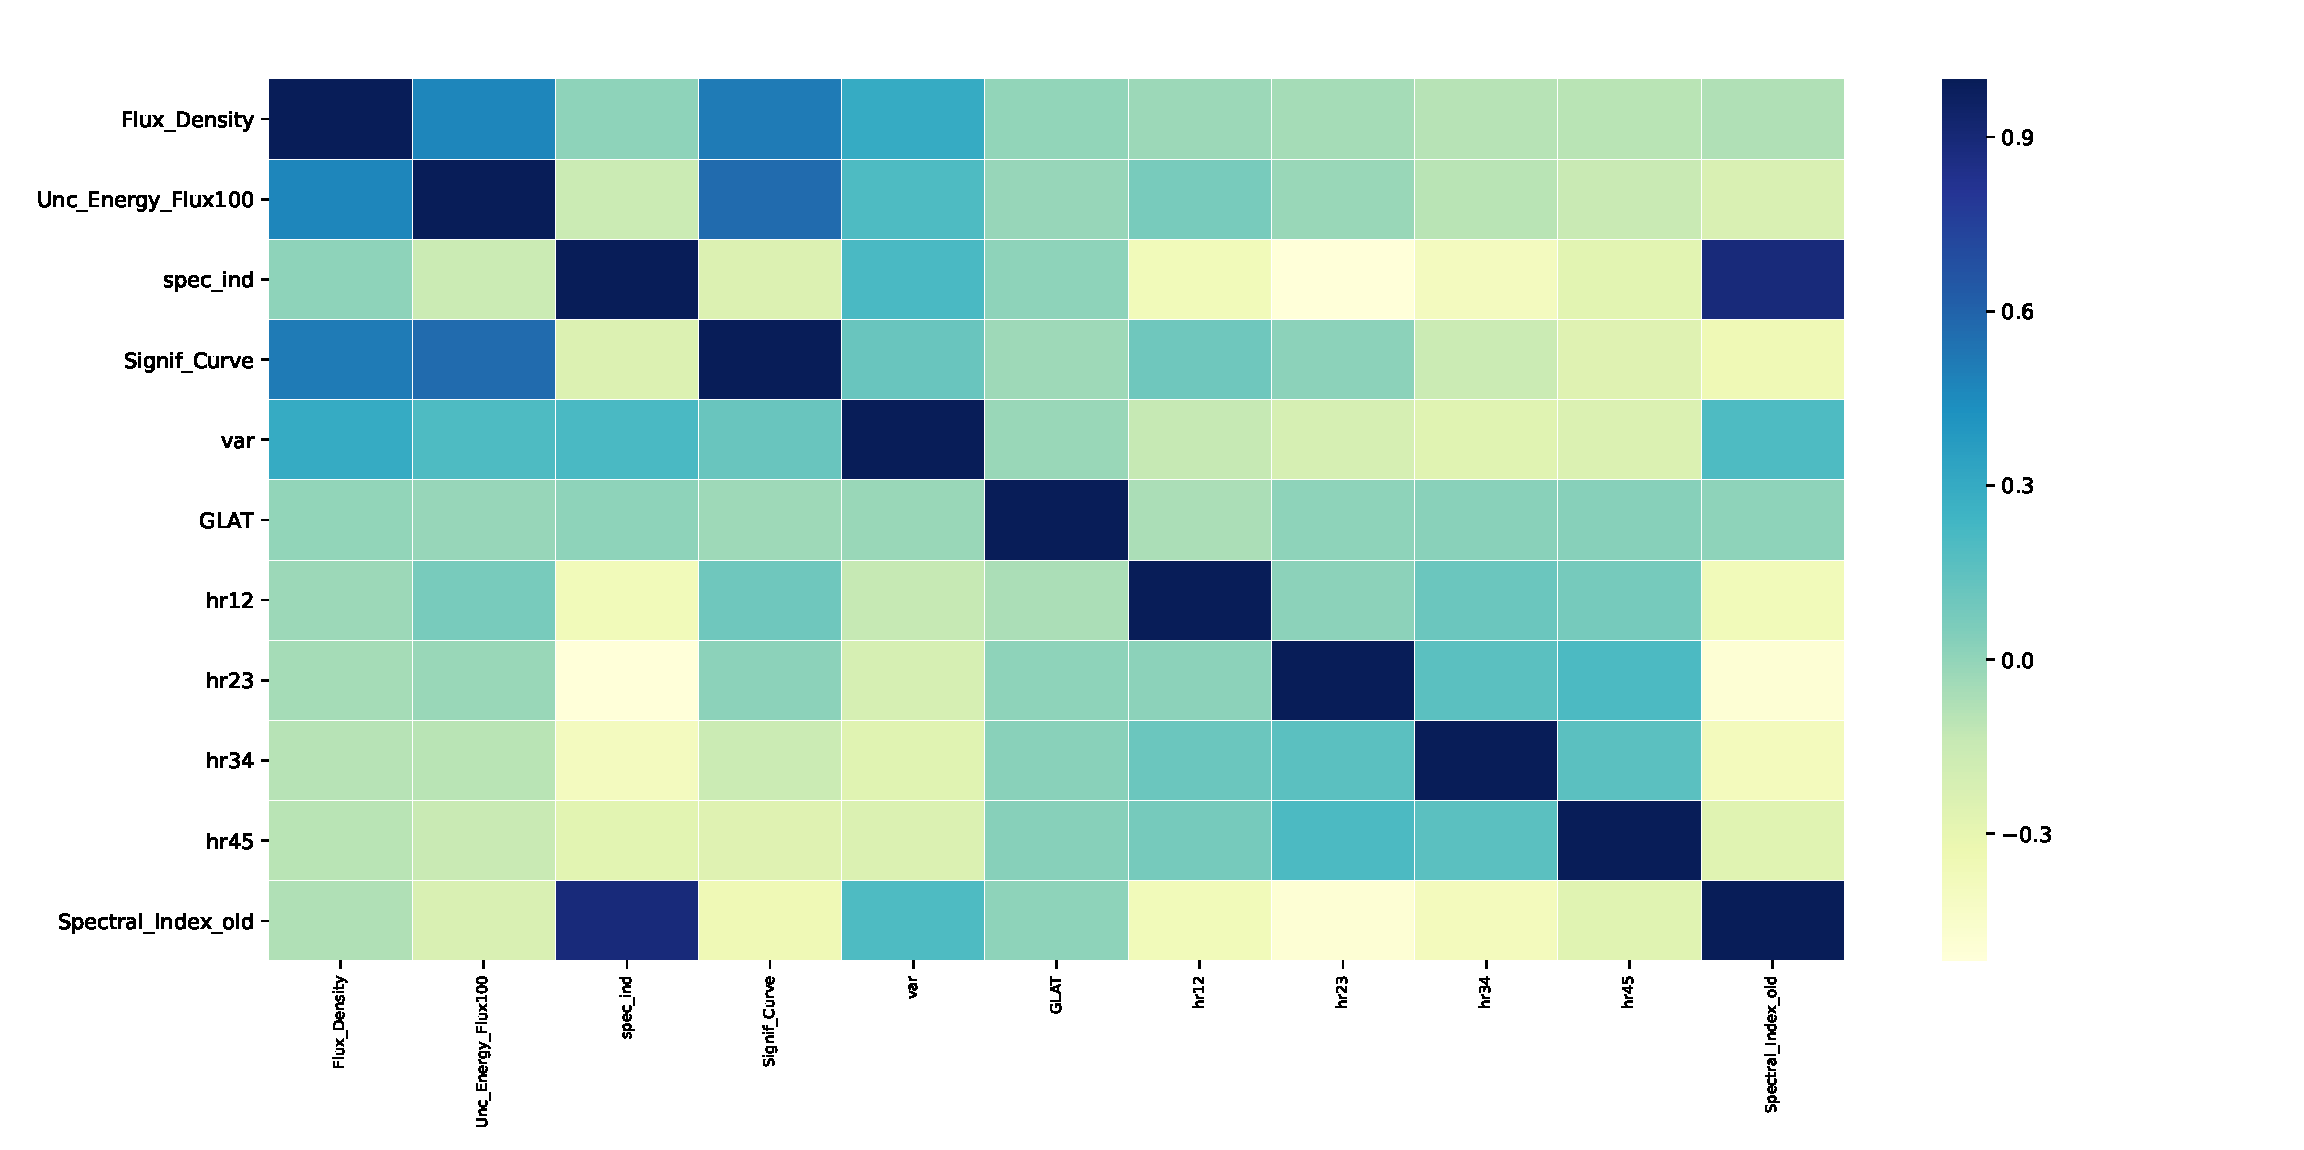
\includegraphics[width=\onepic\textwidth]{plots/correlation.pdf}
\caption{Correlation matrix for the most important features}
\label{fig:corr}
\end{figure}
[Add Table]\\

The features used for our analysis follow the same idea as the previous studies. The features, along with statistical and methodological details, are given below. A correlation matrix is presented for the most important features as well. The matrix is important for the case where there might be redundant features, in which case using only one of the two features would be a better idea.\\




Our initial hypothesis was that certain features would be more important for classification than others. For instance, as shown below, one can see a clear distinction between the regimes of AGNs and Pulsars, based on spectral idex and significant curvature. [Add image] While not clearly obvious from the get go, we were also interested in comparing the importance of features based on the algorithms that we were using. Due to the difference in the basic method of Random Forests and Neural Networks, we expected a slight shift in their reliance on certain features. Despite that we hypothesized that features with the most contribution would be among spectral index, variability, and the curvature; as already observed by Parkinson et. al. This is made clearer by the two figures below, which highlight the separation of PSR and AGN. The separation is seen to be much easier when spectral index and curvature are used, as opposed to the flux and uncertainty on the flux.\\

\begin{figure}[h]
%\centering
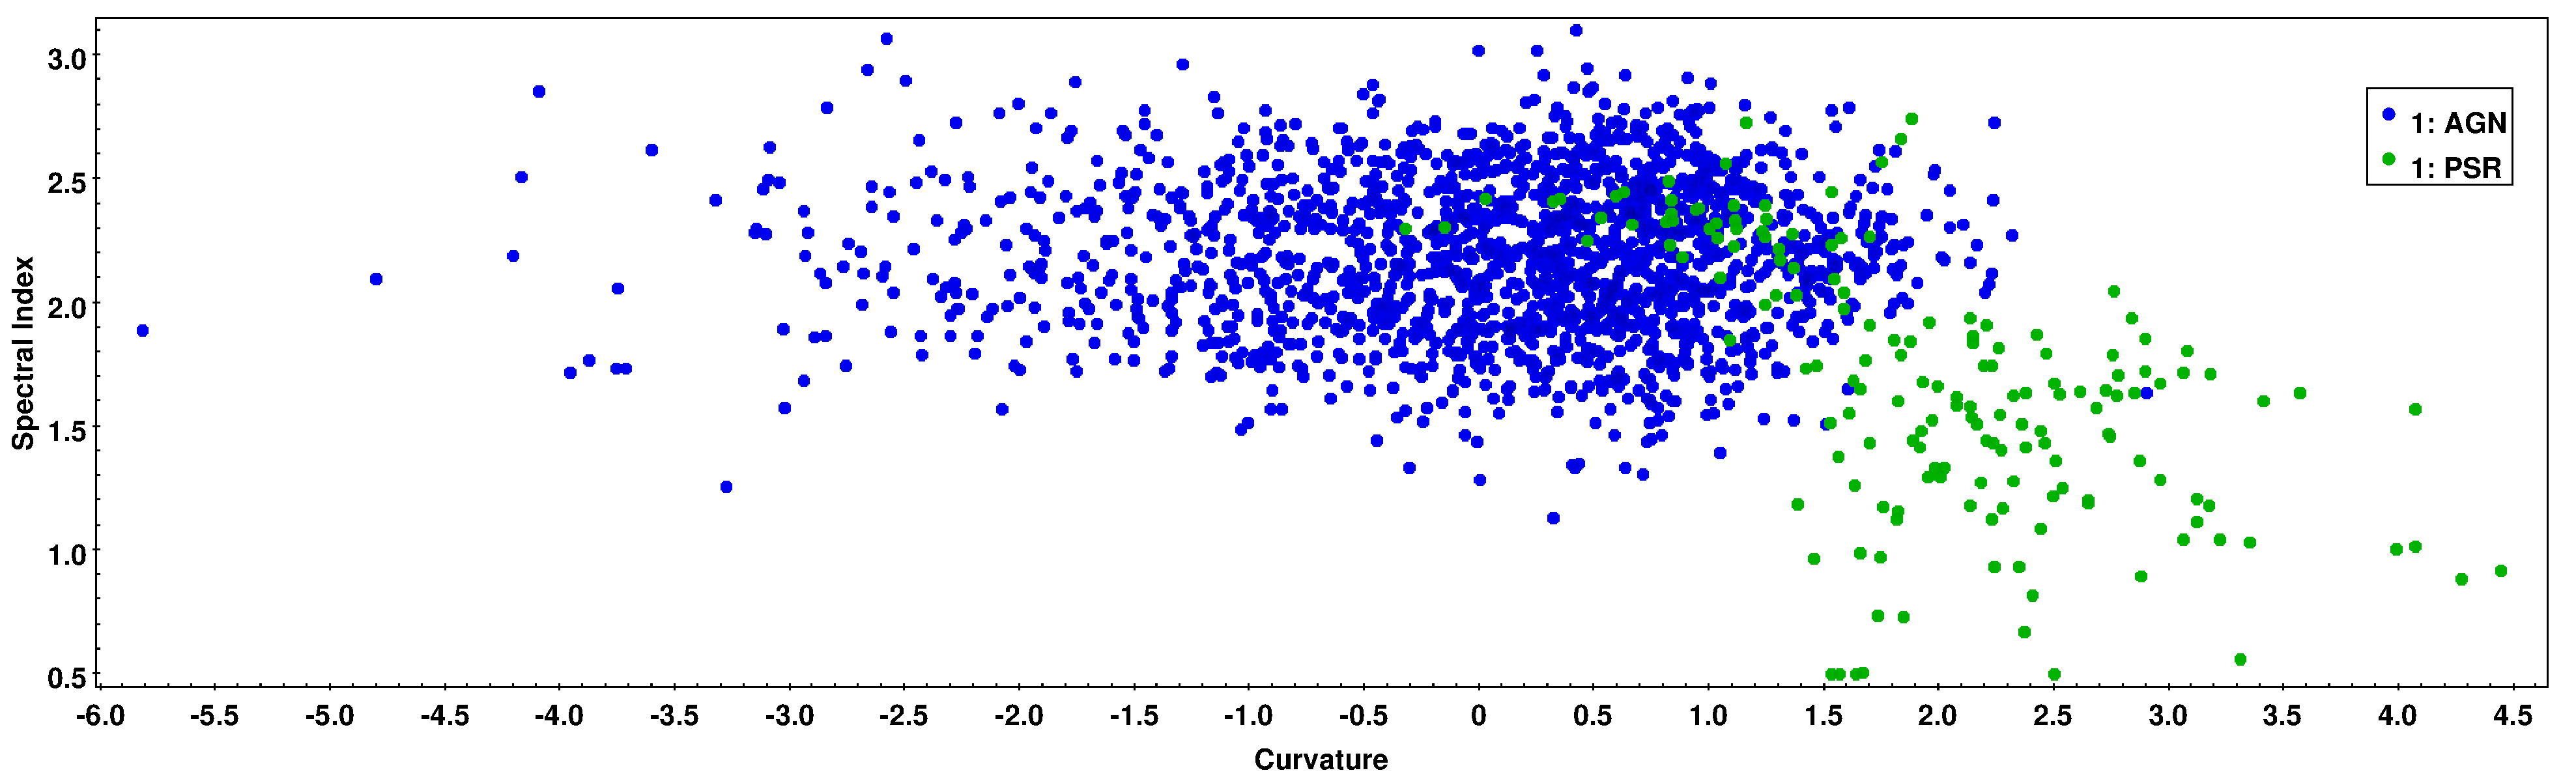
\includegraphics[width=\onepic\textwidth]{plots/signifcurvvsspecind2.pdf}
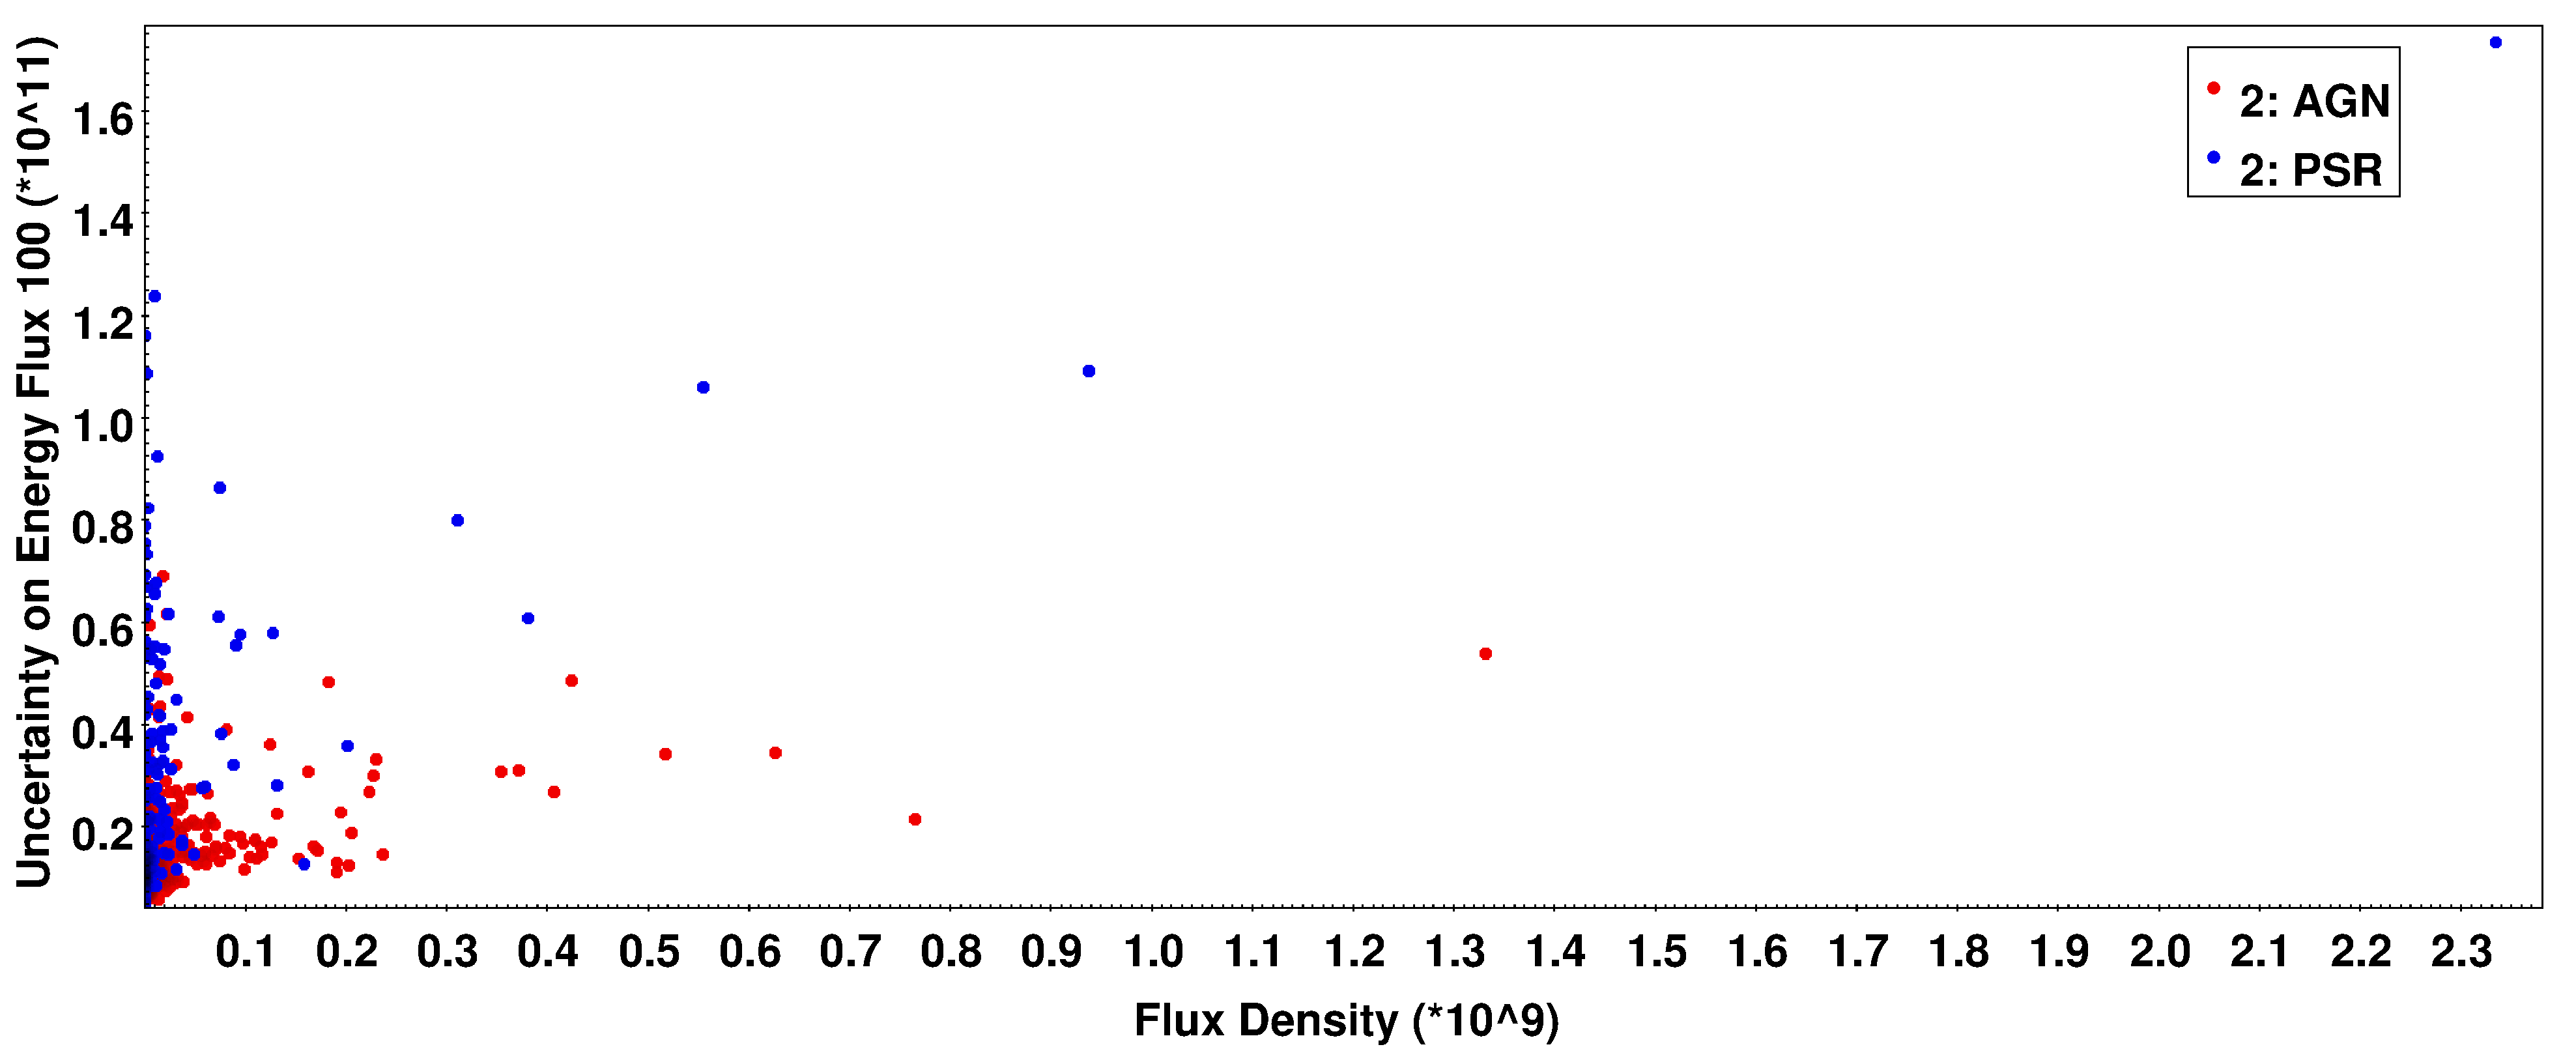
\includegraphics[width=\onepic\textwidth]{plots/fluxvsunc.pdf}
\caption{Separation of AGNs and PSRs from the 3FGL catalog based on different features}
\label{fig:corr}
\end{figure}




These importances were found to be consistent for various different algorithm parameters. So while the value might change a bit for different tree architechtures, for instance, the importances of these features were still pronounced. \\
\subsection{Comparison of the classification algorithms}

\end{comment}

\subsubsection{Random Forests}
\lb{sec:rf}

The two main parameters characterizing the random forest algorithm are the number of trees and the maximum depth allowed in these trees. 
We use the Gini index as the objective function for the optimization of parameters (split values of features in the nodes).
Since the number of pulsars is about 10 times smaller than AGNs,
we consider two cases of weighting the input data:
equal weights -- all PS have equal weights in the objective function, and inverse weighting -- the contribution of the PS is inversely proportional to the total number of elements in the class, in this case the contribution of a pulsar is more significant than the contribution of an AGN so that the overall contributions of pulsars and AGNs to the objective function are similar.

\begin{figure}[h]
%\centering
\hspace*{-0.5cm}
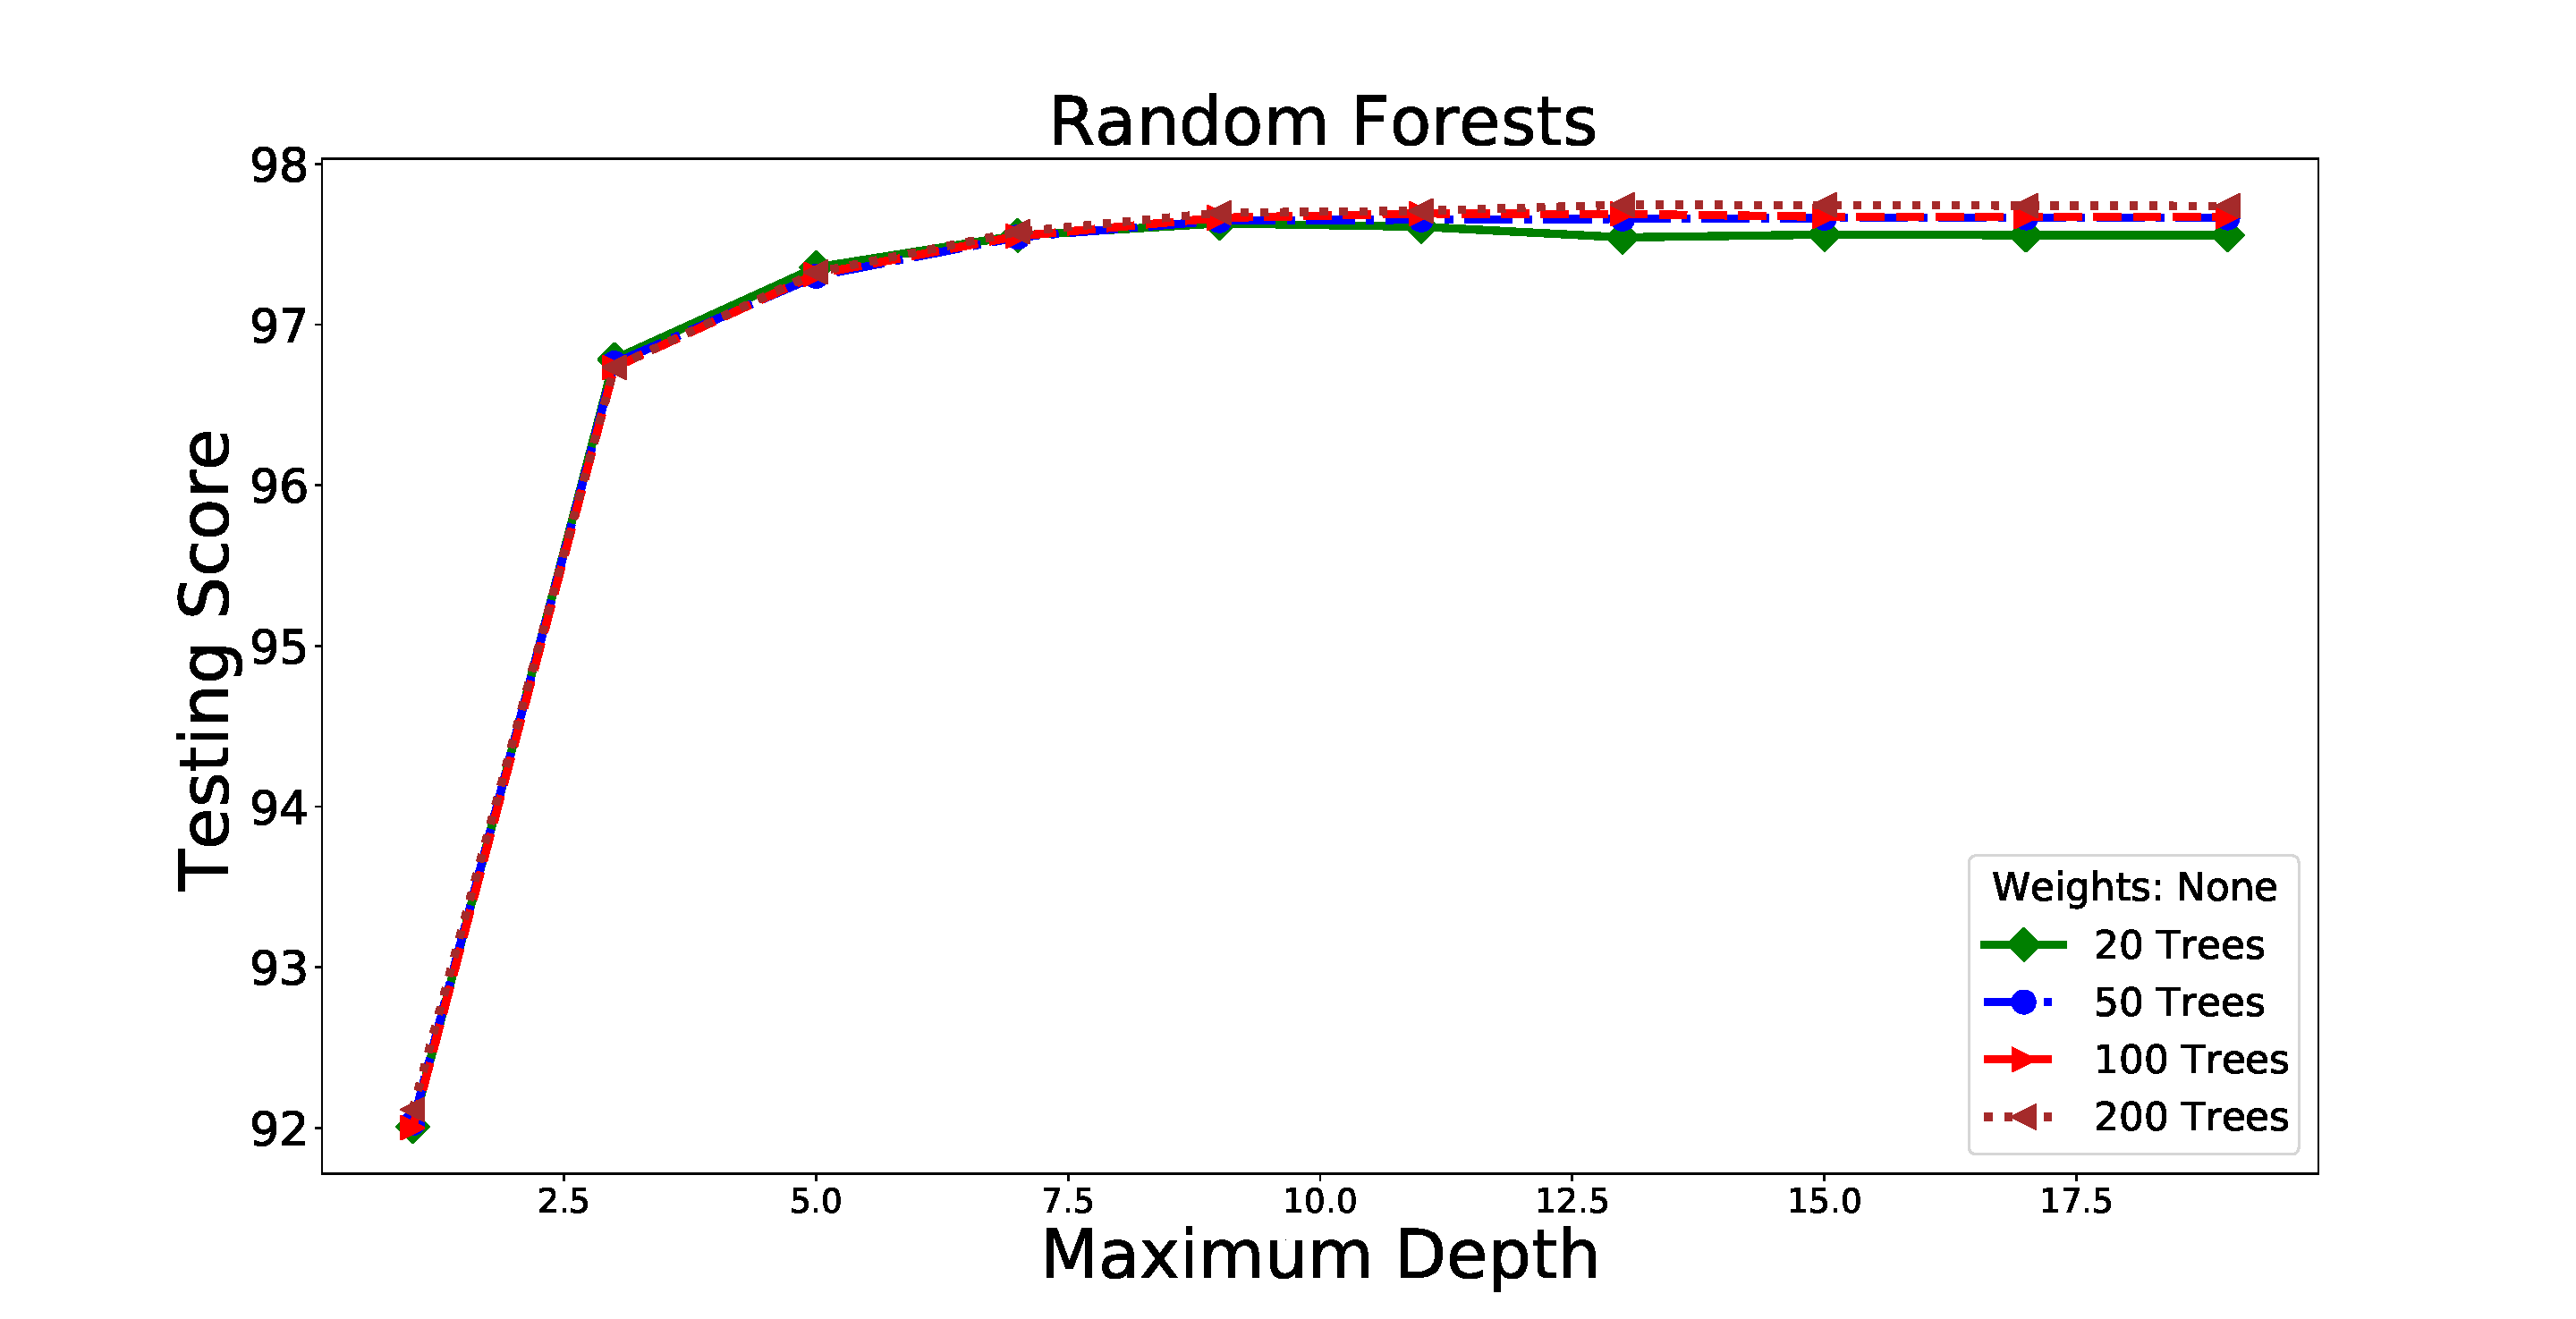
\includegraphics[width=0.5\textwidth]{plots/rf_train_unweighted}
\hspace*{-0.5cm}
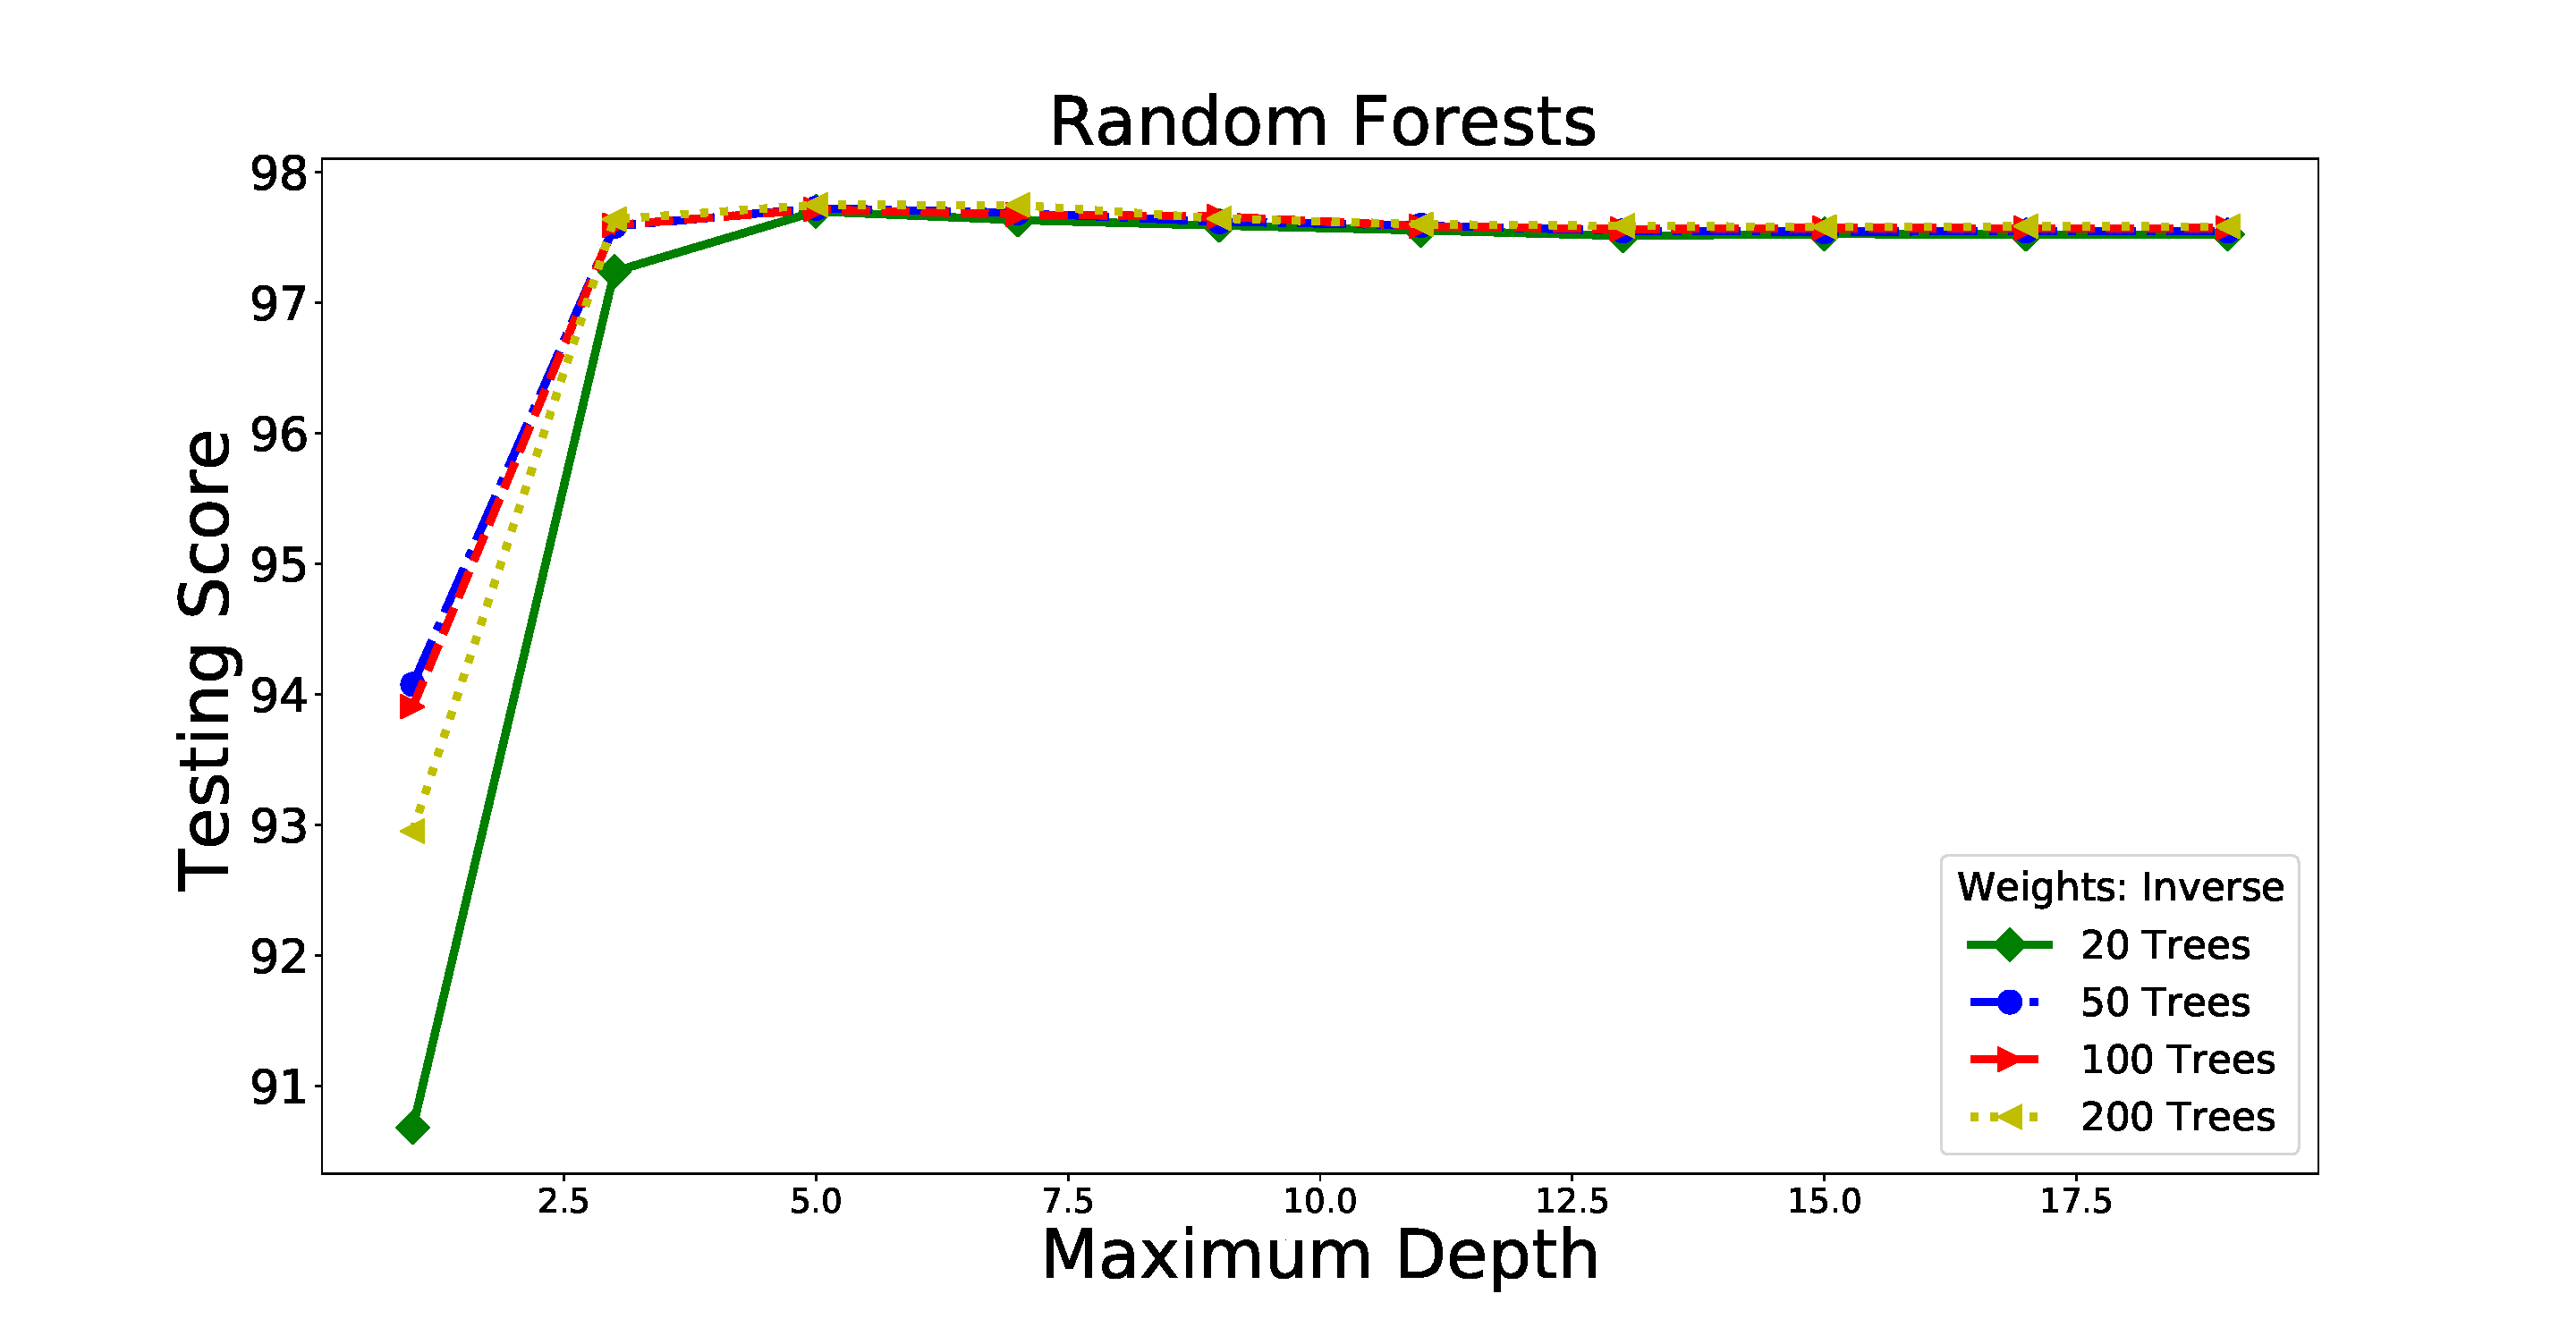
\includegraphics[width=0.5\textwidth]{plots/rf_train_weighted}
%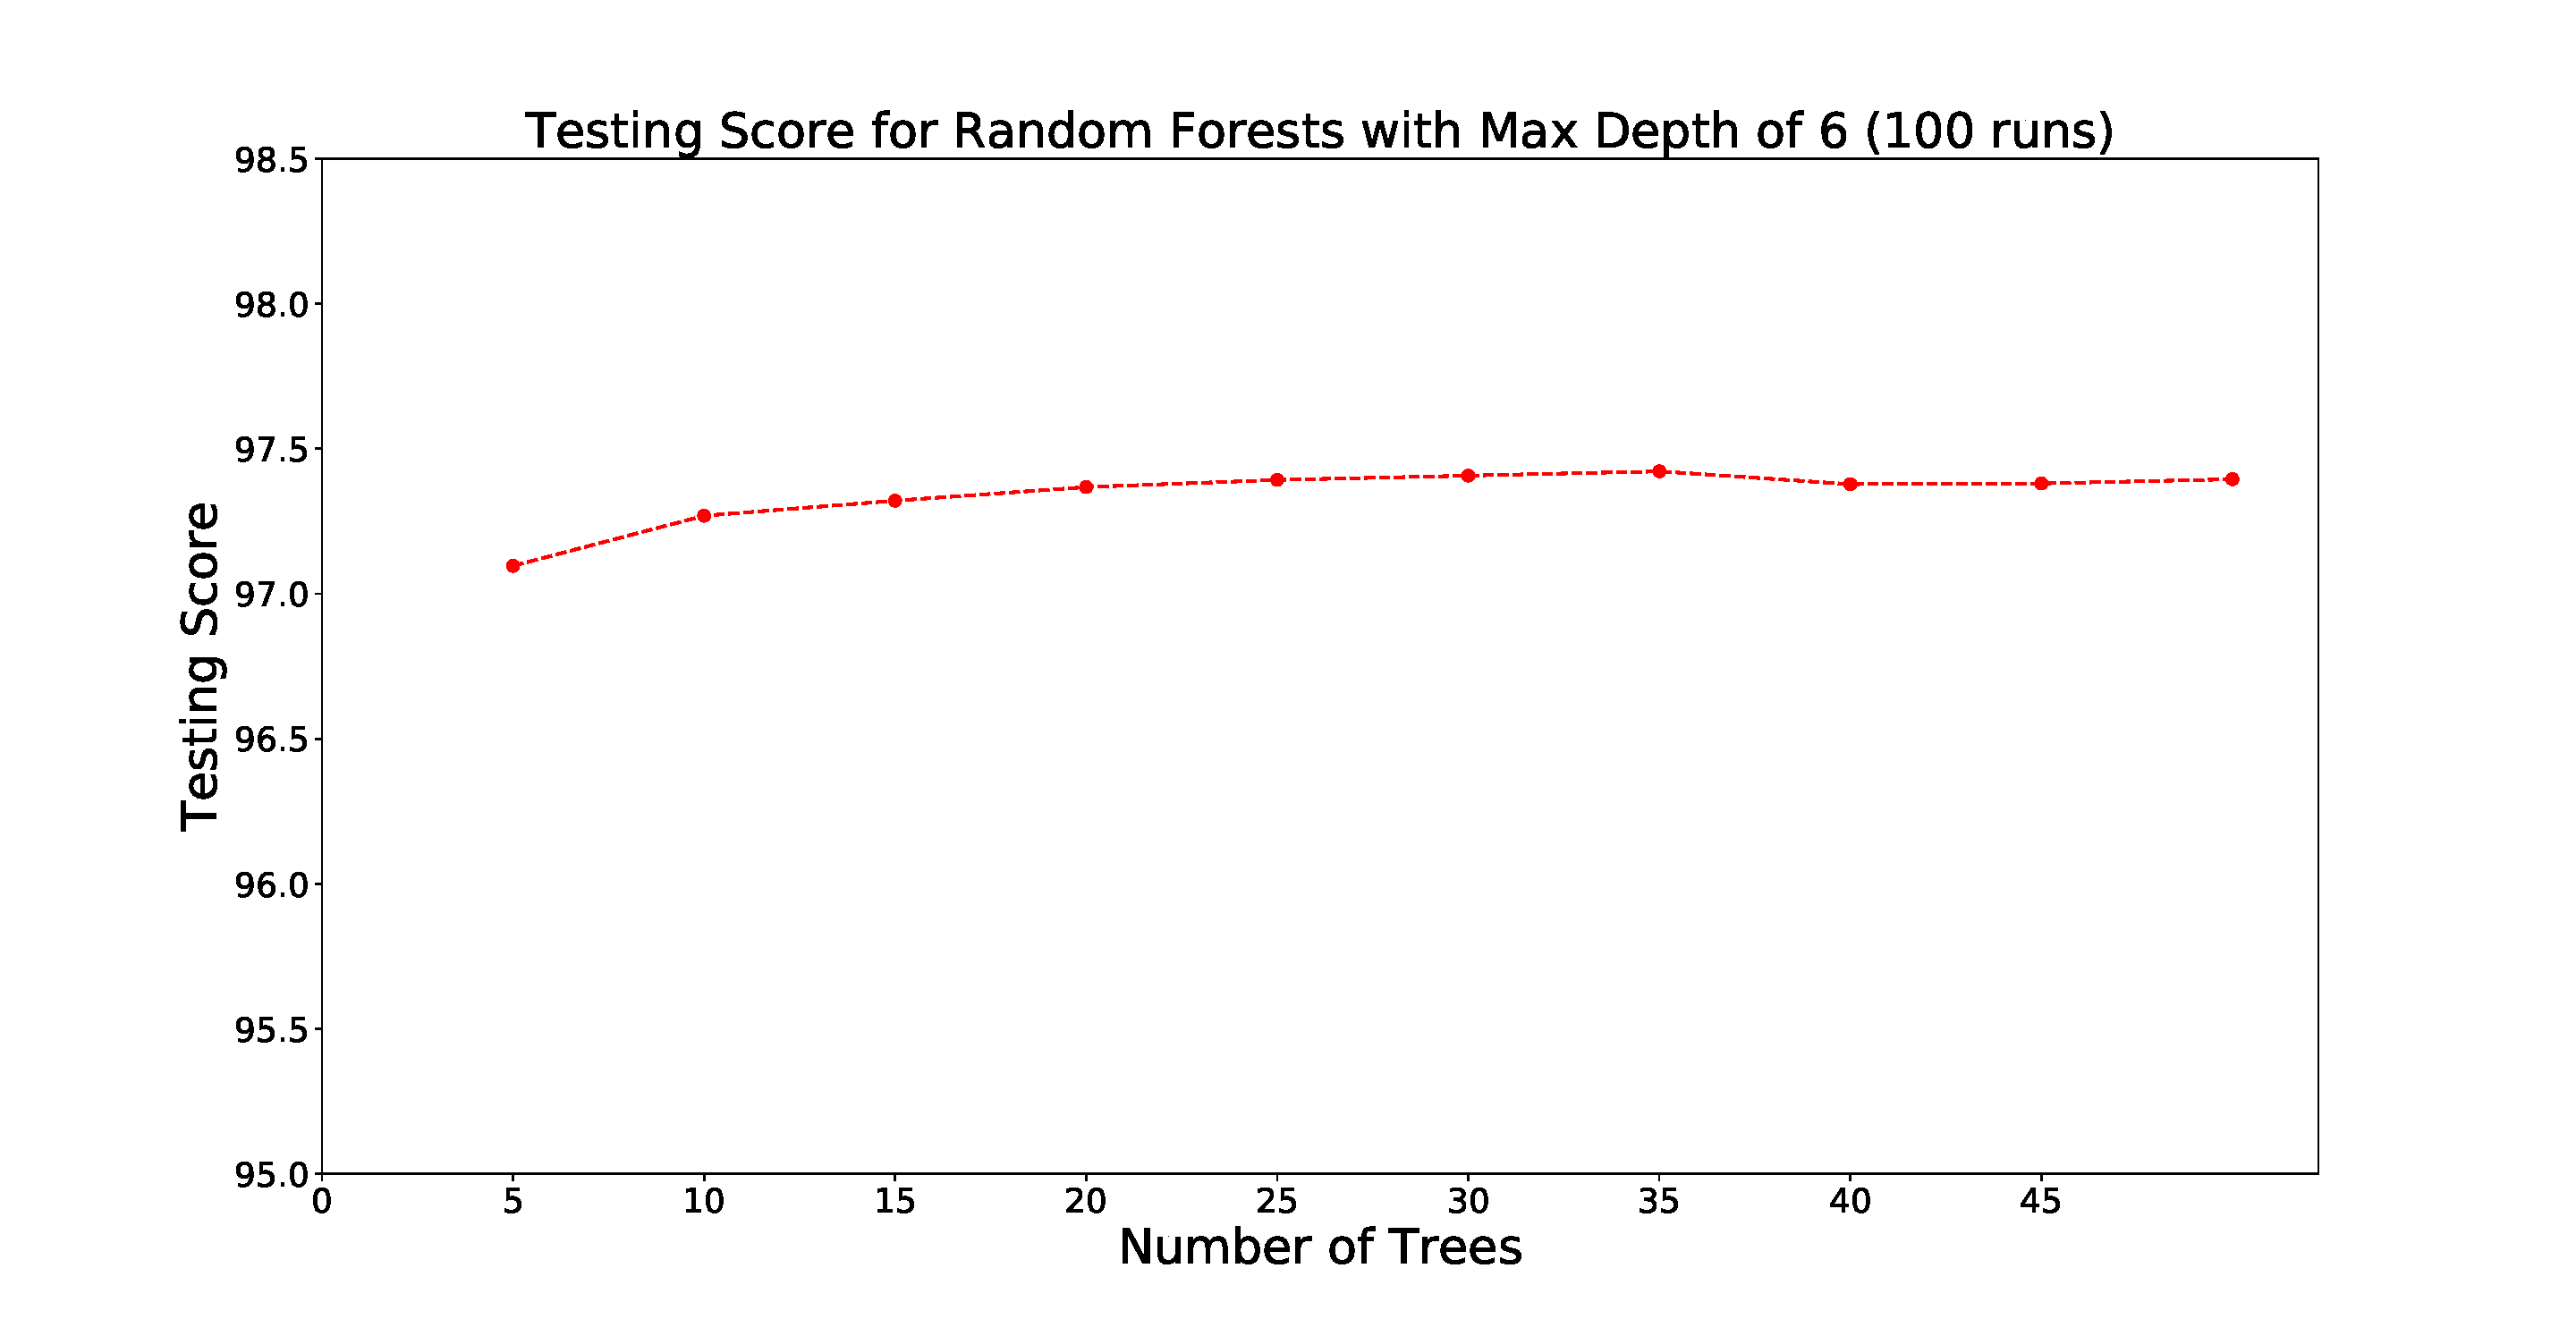
\includegraphics[width=\twopicsp\textwidth]{plots/6md_trees_weighted}
\caption{
Test score of RF classification as a function of the number of trees and maximal depth of trees for weighted and unweighted training data.
%\dima{Add ``weighted'' in the figure title, e.g., ``Random forests with weighted dat'', in order to make consistent titles in the two plots.}
}
\label{fig:RF_complexity}
\end{figure}

Figure \ref{fig:RF_complexity} shows the dependence of the accuracy of the test sample as a function of maximum depth and the number of trees. 
The results for each point are averaged over 100 realizations of the split into training and testing samples.
%We perform weighting of the data by the inverse numbers of pulsars and AGNs to take into account that there are more AGNs than pulsars. However, for random forests, 
As one can see from this figure,
weighting the training data does not have a significant effect on the accuracy of PS classification into pulsars and AGNs.
We also notice that the test score does not decrease significantly with a larger complexity of the model, e.g., there is little change in accuracy for maximal depths above $\sim$ 5.
This is due to the random choice of a subset of features (maximum number of allowed features is $\sqrt{\text{features}}$) at each node.
Furthermore, we find that the number of trees is not as important as the depth: a lower number of trees does not significantly change the accuracy, above, e.g., 20 for unweighted data (Figure \ref{fig:RF_complexity}). 
%However, a lower depth certainly lessens the accuracy significantly, and therefore this threshold must be chosen carefully.
%In the case of training, we found no significant differences when using weights for our data set. However, we chose to use a inversely weighted dataset since that allows us to generalize the algorithm more. The influence of weights will also be discussed more in the case of unassociated data, in the next section.
%After running tests on various architectures we chose a Random Forest with 20 trees to avoid over-fitting, and a maximum depth of 12.
%\dima{
%Why 12? It looks like 4 or 5 is already good enough.
%We should write here an equation for test score in case of weighted data.}

In tree-based algorithms, one can calculate feature importance by using the averaged reduction of impurity for nodes involving the different features. The feature importances for the case of two different RF algorithms: 20 trees with max depth of 2 and 50 trees with max depth of 6 are shown in Table \ref{tab:feat_imp}.
We find that the three most important features for both cases are significance of curvature, hardness ratio of the last two energy bins, and spectral index (shown in bold font in the table).
%Since Random forests are based on decision trees, they allow us to characterize feature importances based on how helpful a feature was to split a tree. In our case, using all 10 features discussed above we found the following feature importances for two architectures of random forests with similar accuracies of 97.5:\\


\begin{table}[!h]
    \tiny
    \centering
    \renewcommand{\tabcolsep}{1mm}
\renewcommand{\arraystretch}{1}

    \begin{tabular}{|c|c|c|}
    \hline
    Feature &  20 trees, depth 2& 50 trees, depth 6\\
    \hline
    $\ln$(Flux\_Density) & 0.04 & 0.05        \\
    \hline
    $\ln$(Unc\_Energy\_Flux100) & 0.07     & 0.08 \\
    \hline %\midrule   -> aakash do you mean this?
   {\bf Spectral\_Index} & 0.13     &   0.11\\
    \hline %\midrule   -> aakash do you mean this?
    {\bf $\ln$(Signif\_Curve)} & 0.33 &0.29  \\
    \hline
   $\ln$(Variability\_Index)&  0.06   &  0.10  \\
    \hline %\midrule   -> aakash do you mean this?
    hr12& 0.03 &0.03 \\
    \hline
     hr23& 0.03 &0.04 \\
    \hline
    hr34& 0.02 &0.03 \\
    \hline
   {\bf hr45} & 0.25 &0.21 \\
    \hline
    GLAT&0.01&0.02\\
    \hline
    \end{tabular}
    \vspace{0.4cm}
    \caption{Feature importances for two RF algorithms.}
    \label{tab:feat_imp}
\end{table}

%Our hypothesis about feature importances turned out to be correct, as curvature, variability, and spectral index were the most important features. The last hardness ratio was also seen to be quite important, most probably reflecting the end of the spectrum where the AGNs and PSRs shift from each other.\\
It is interesting to note that Galactic latitude is the least significant feature.
We have also used sine of GLAT to check that this is not due to scaling, i.e., the large range of values of GLAT,
but the significance is similar to the GLAT itself.

In order to illustrate the separation of the PS into AGNs and PSRs, we retrain the RF algorithm using only two features: log of curvature significance and spectral index, and plot the resulting probabilities of classes in Figure \ref{fig:RF_domains}. 
These classification domains illustrate the separation of class probabilities.
In our case, it can be seen that depth 6 outperforms depth 2 due to the much more nuanced probability distribution of the model. It is important to note here that this plot is for only one run and the model is trained on two features,
however, it shows why the higher depth outperforms the lesser one. 
%The higher the depth the more the probabilities becomes denser and the dense areas become smaller. For instance, one can see regions of near zero probabilities in the depth of 6 as opposed to a depth of 2. 
It also illustrates how more complex algorithms can over-fit the data (notice the narrow bands in probability distribution for max depth of 6 case),
although overfitting is not an issue for RF algorithms in our case.
%This situation is not so obvious for random forests, since random forests are especially good against over-fitting. 
%However, we she shall see how other algorithms can over-fit instead.
For the final algorithm, we will use a RF with 50 trees and a maximum depth of 6.
%\dima{Add discussion of the domains, e.g., overfitting, and selection of the final model for classification.}

\begin{figure}[h]
\hspace*{-1cm}
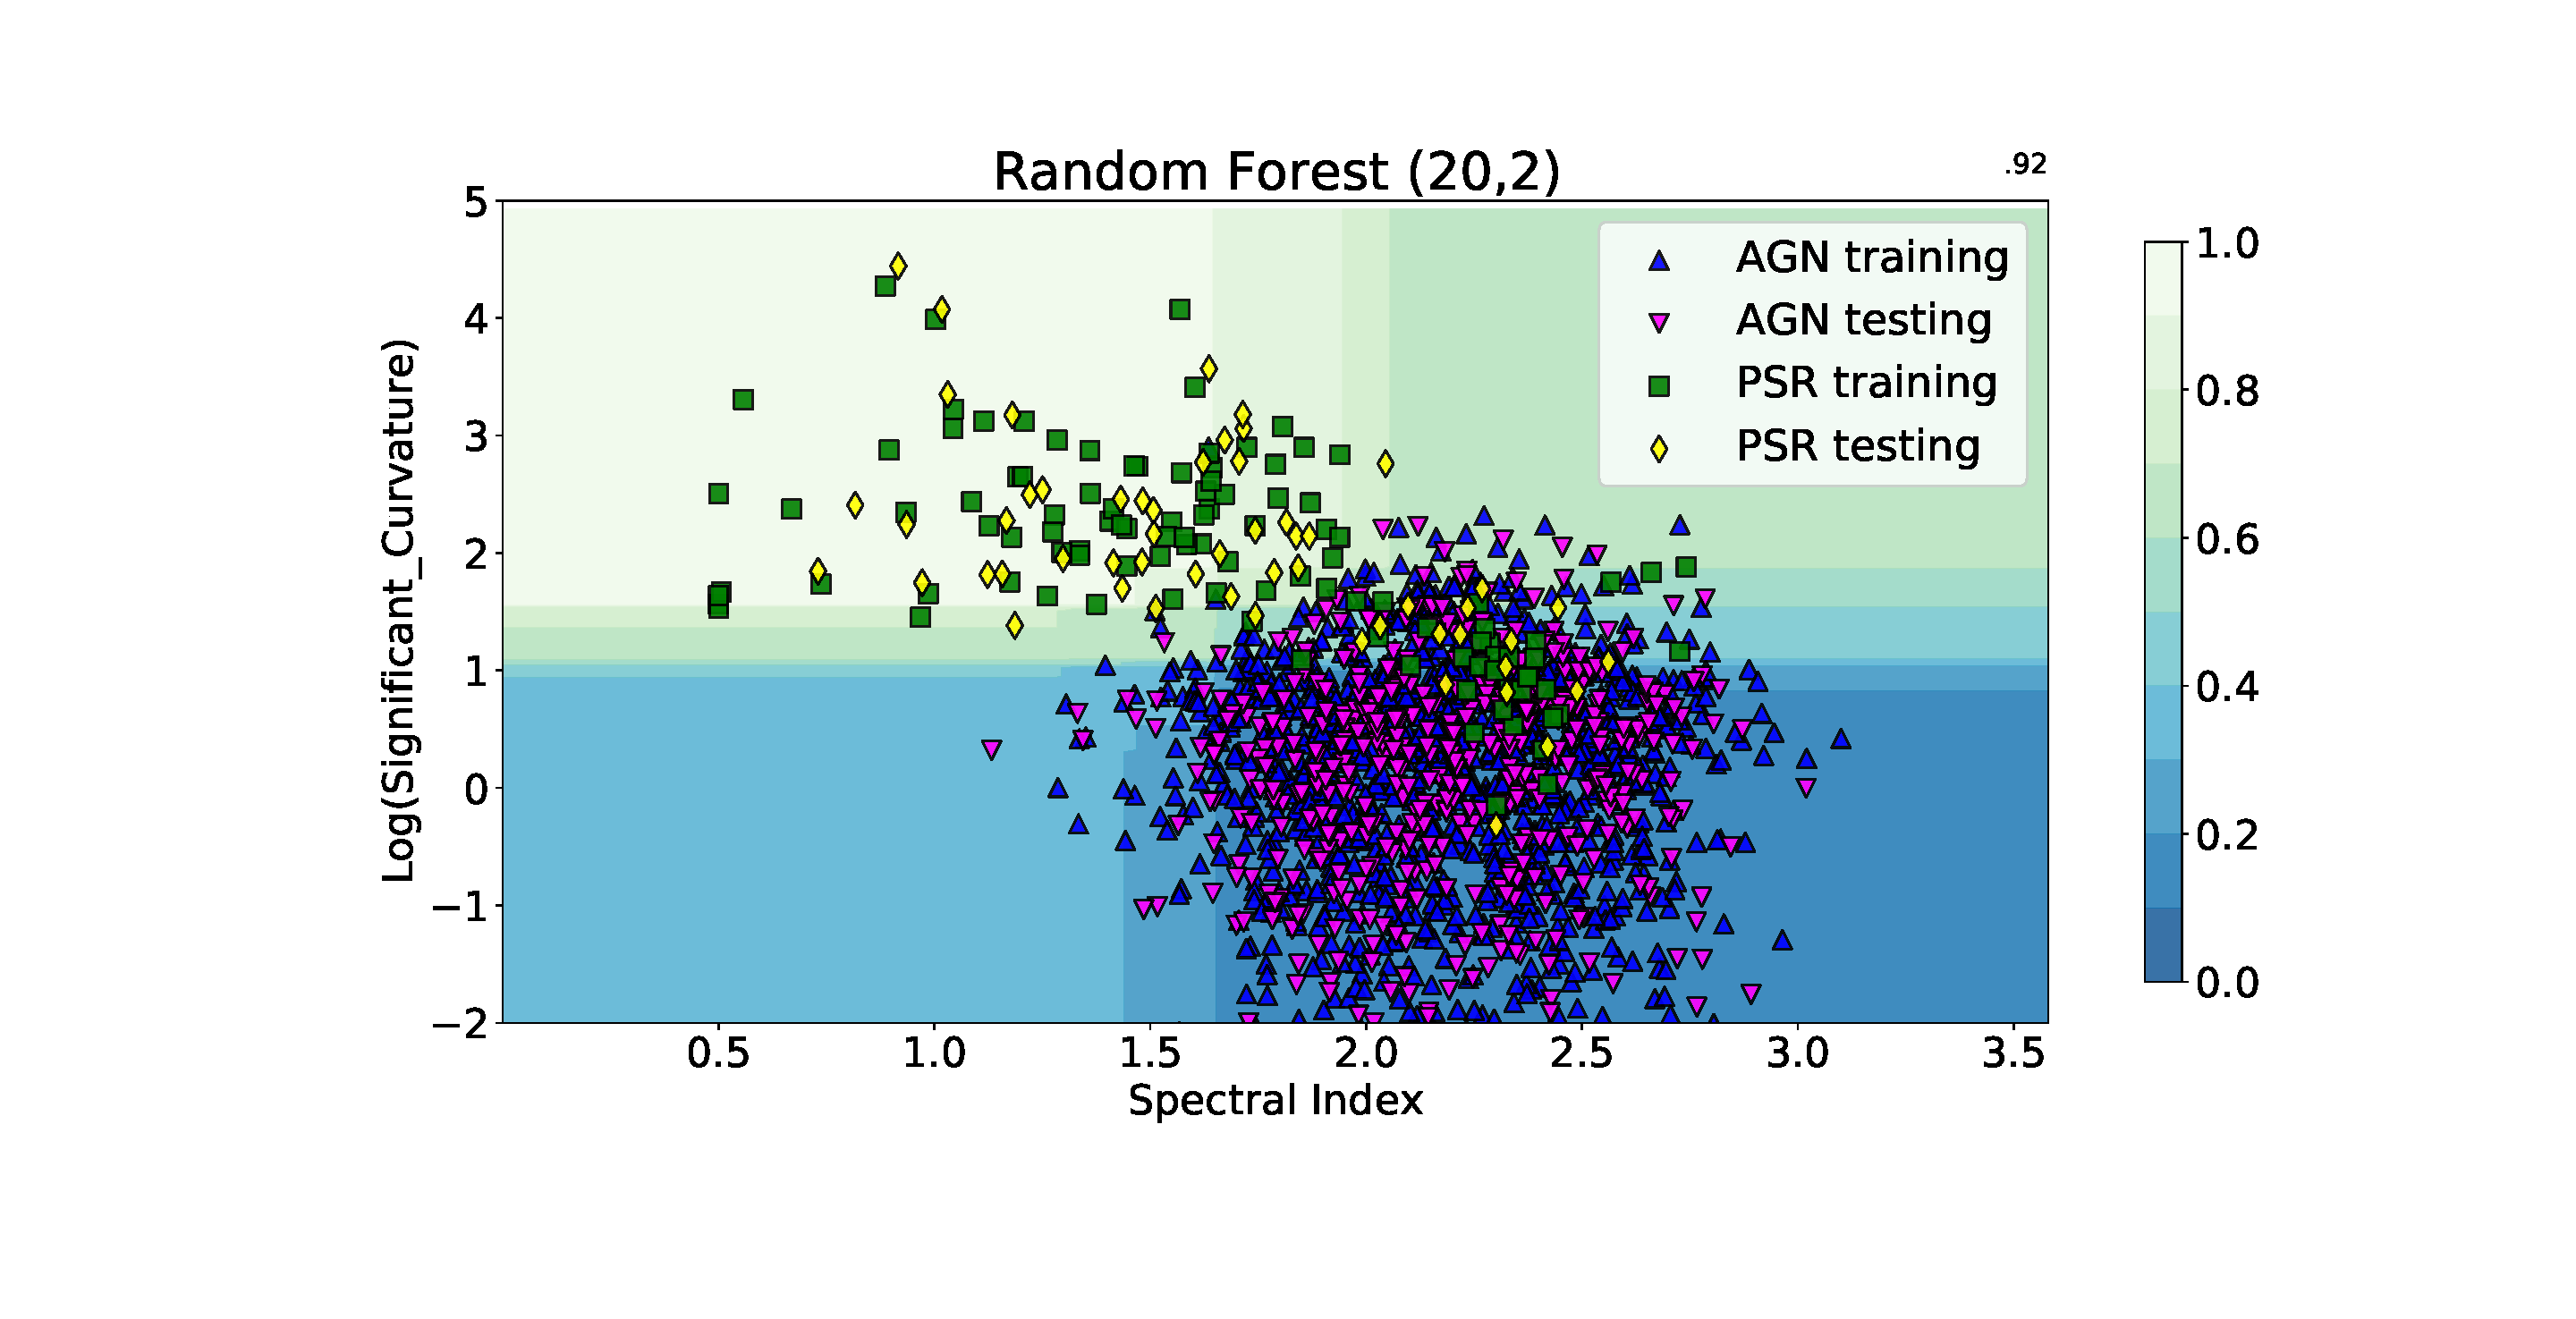
\includegraphics[width=0.6\textwidth]{plots/classification_domains/rf_20_2_final.pdf}
\hspace*{-1cm}
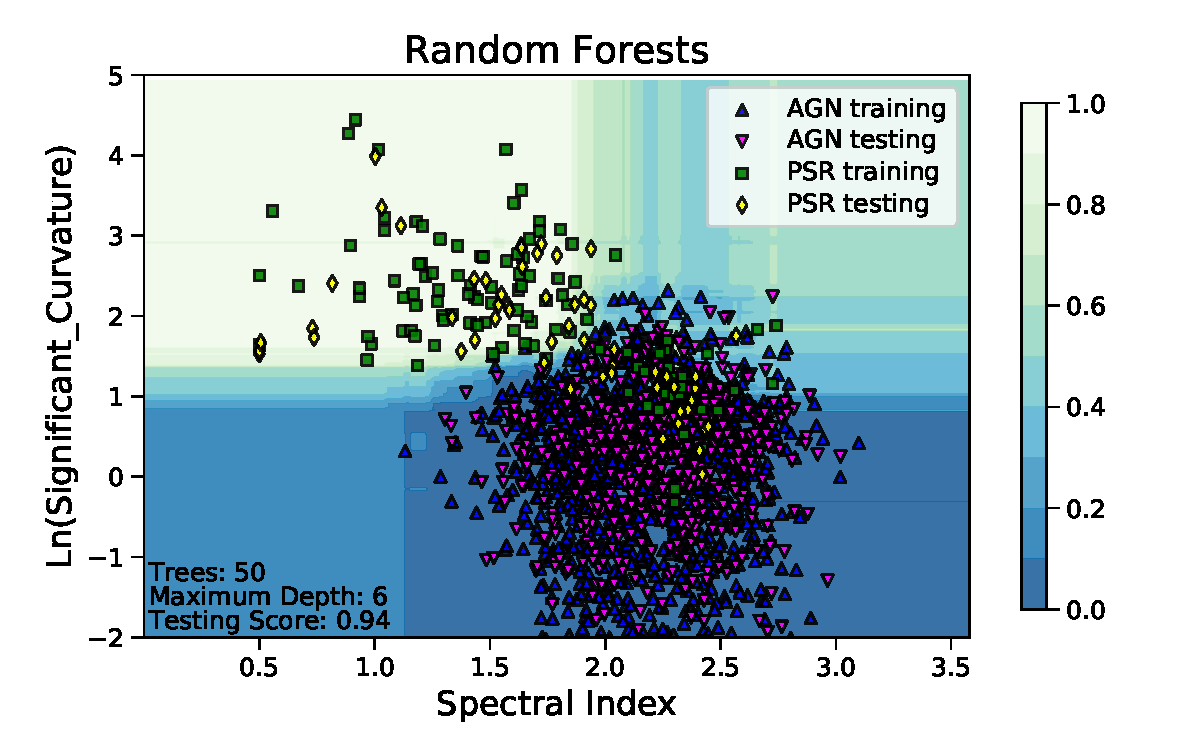
\includegraphics[width=0.6\textwidth]{plots/classification_domains/rf_50_6_final.pdf}
\caption{Classification domains for the RF algorithm: differences in probability distribution as a function of maximum depth and the number of trees in the forest.}  
\label{fig:RF_domains}
\end{figure}

%=======
%\begin{figure*}[h]
%\centering
%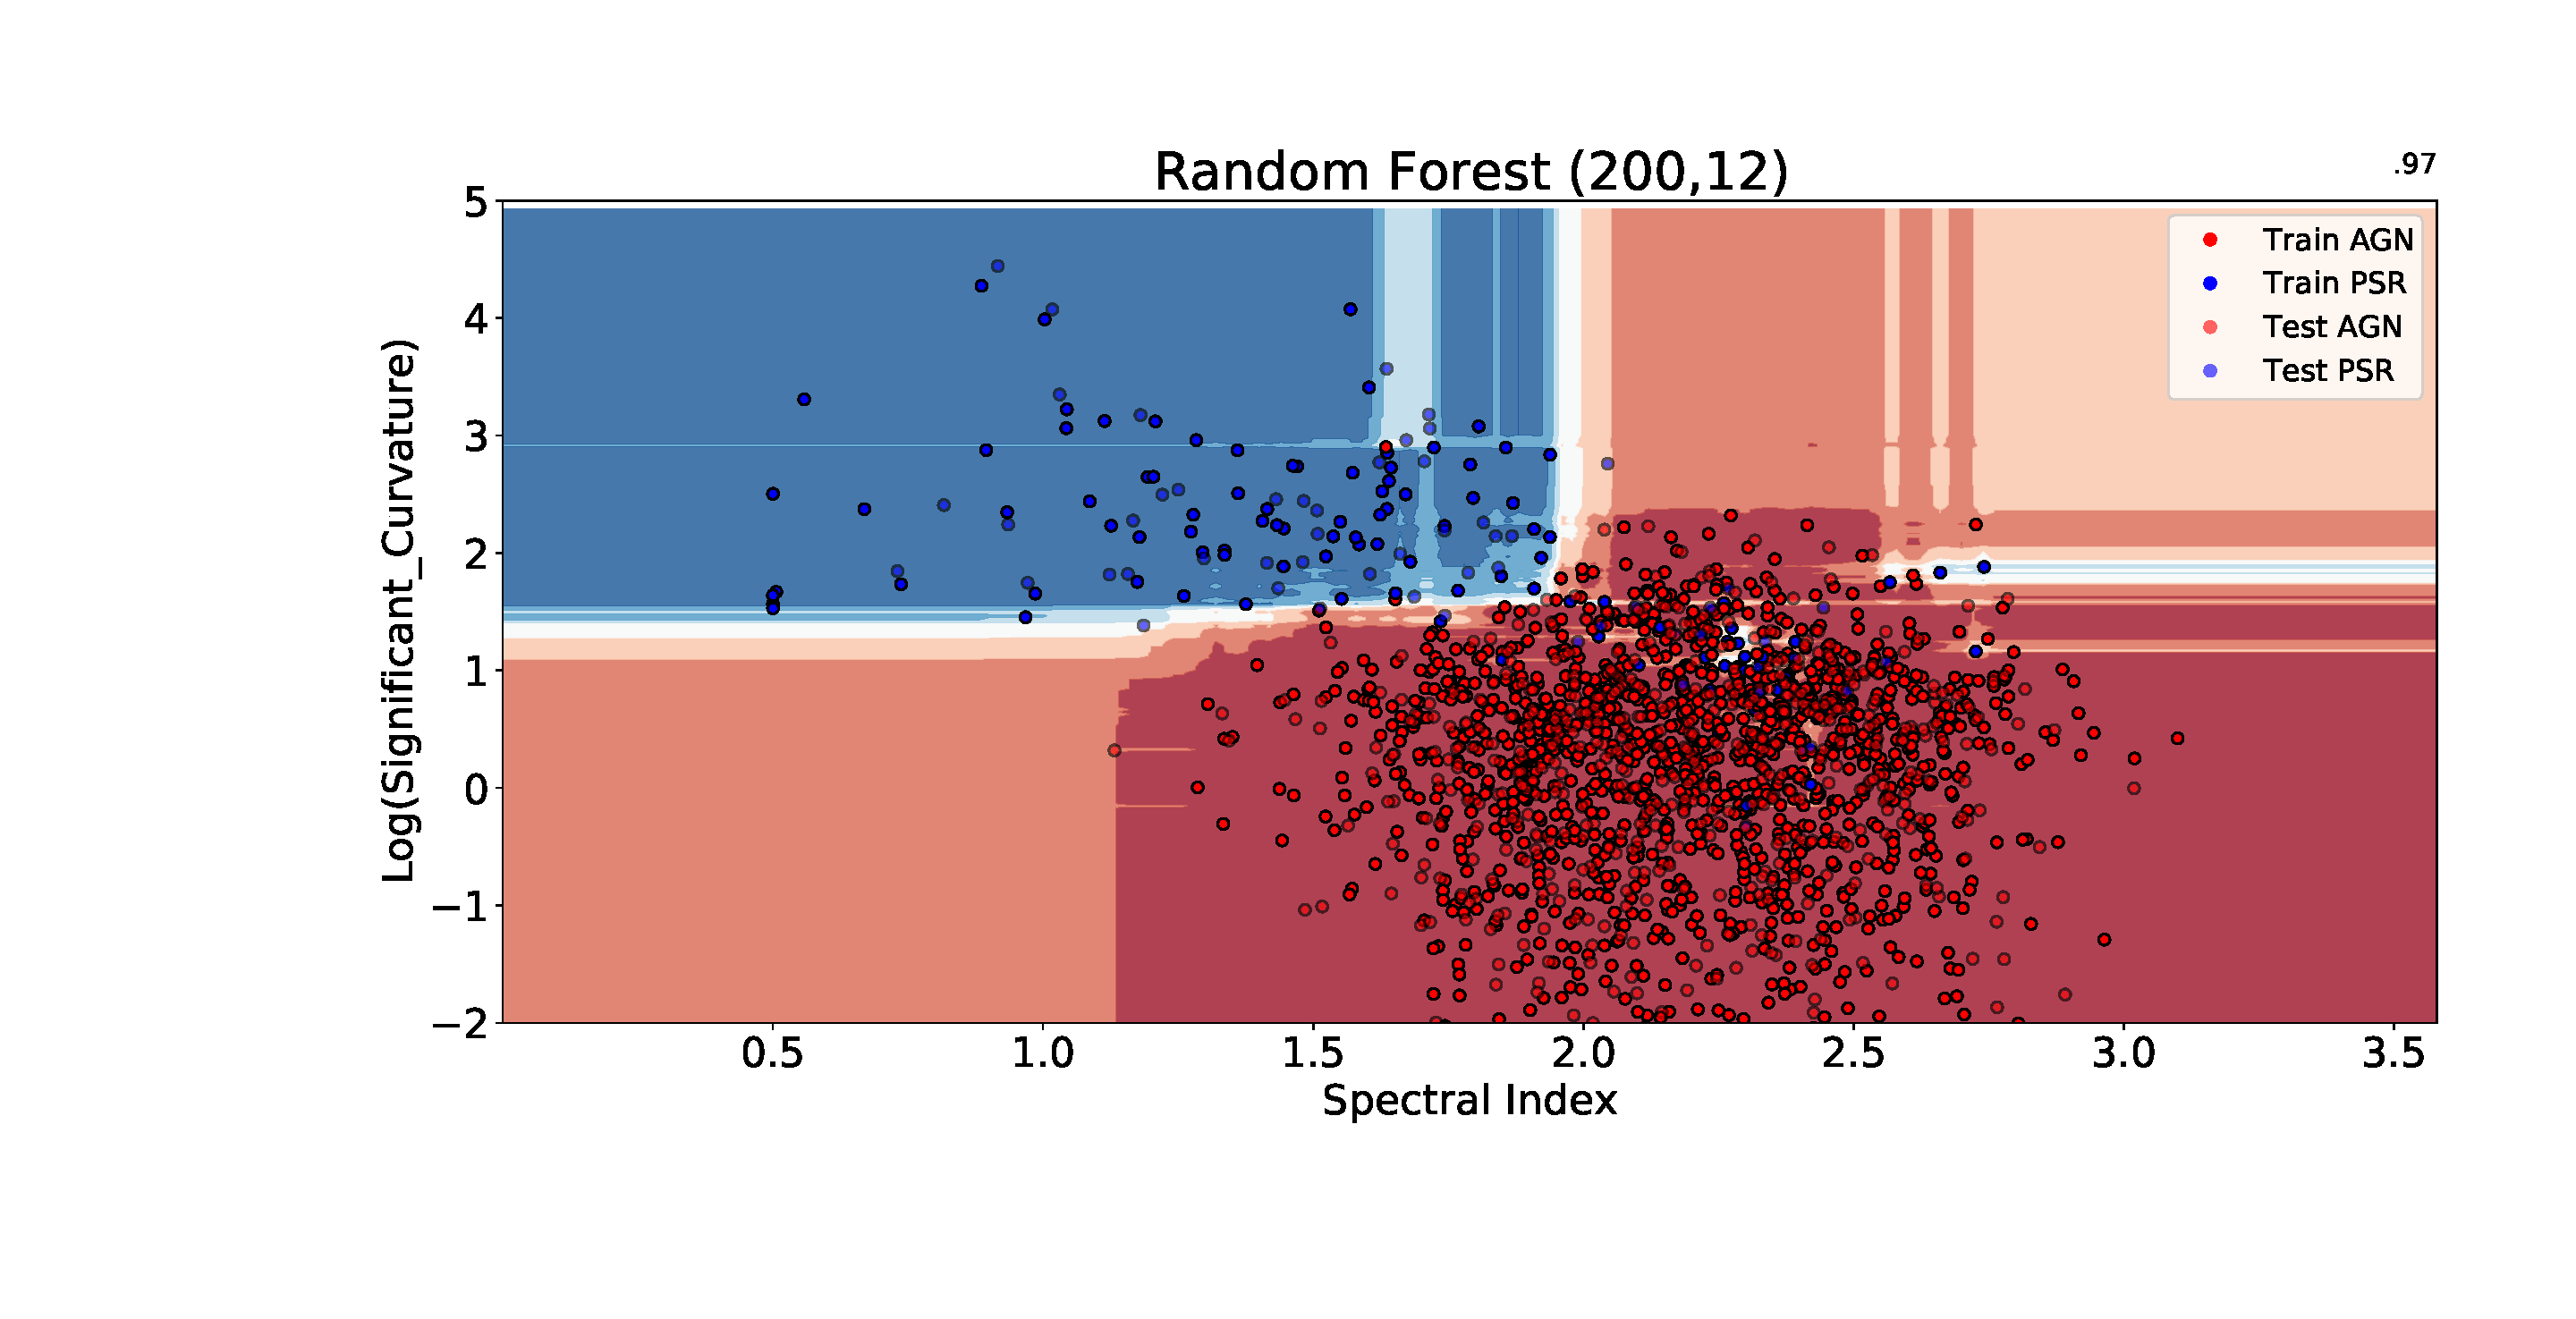
\includegraphics[width=\twocolumnwidth\textwidth]{plots/classification_domains/rf_200_12.pdf}\\
%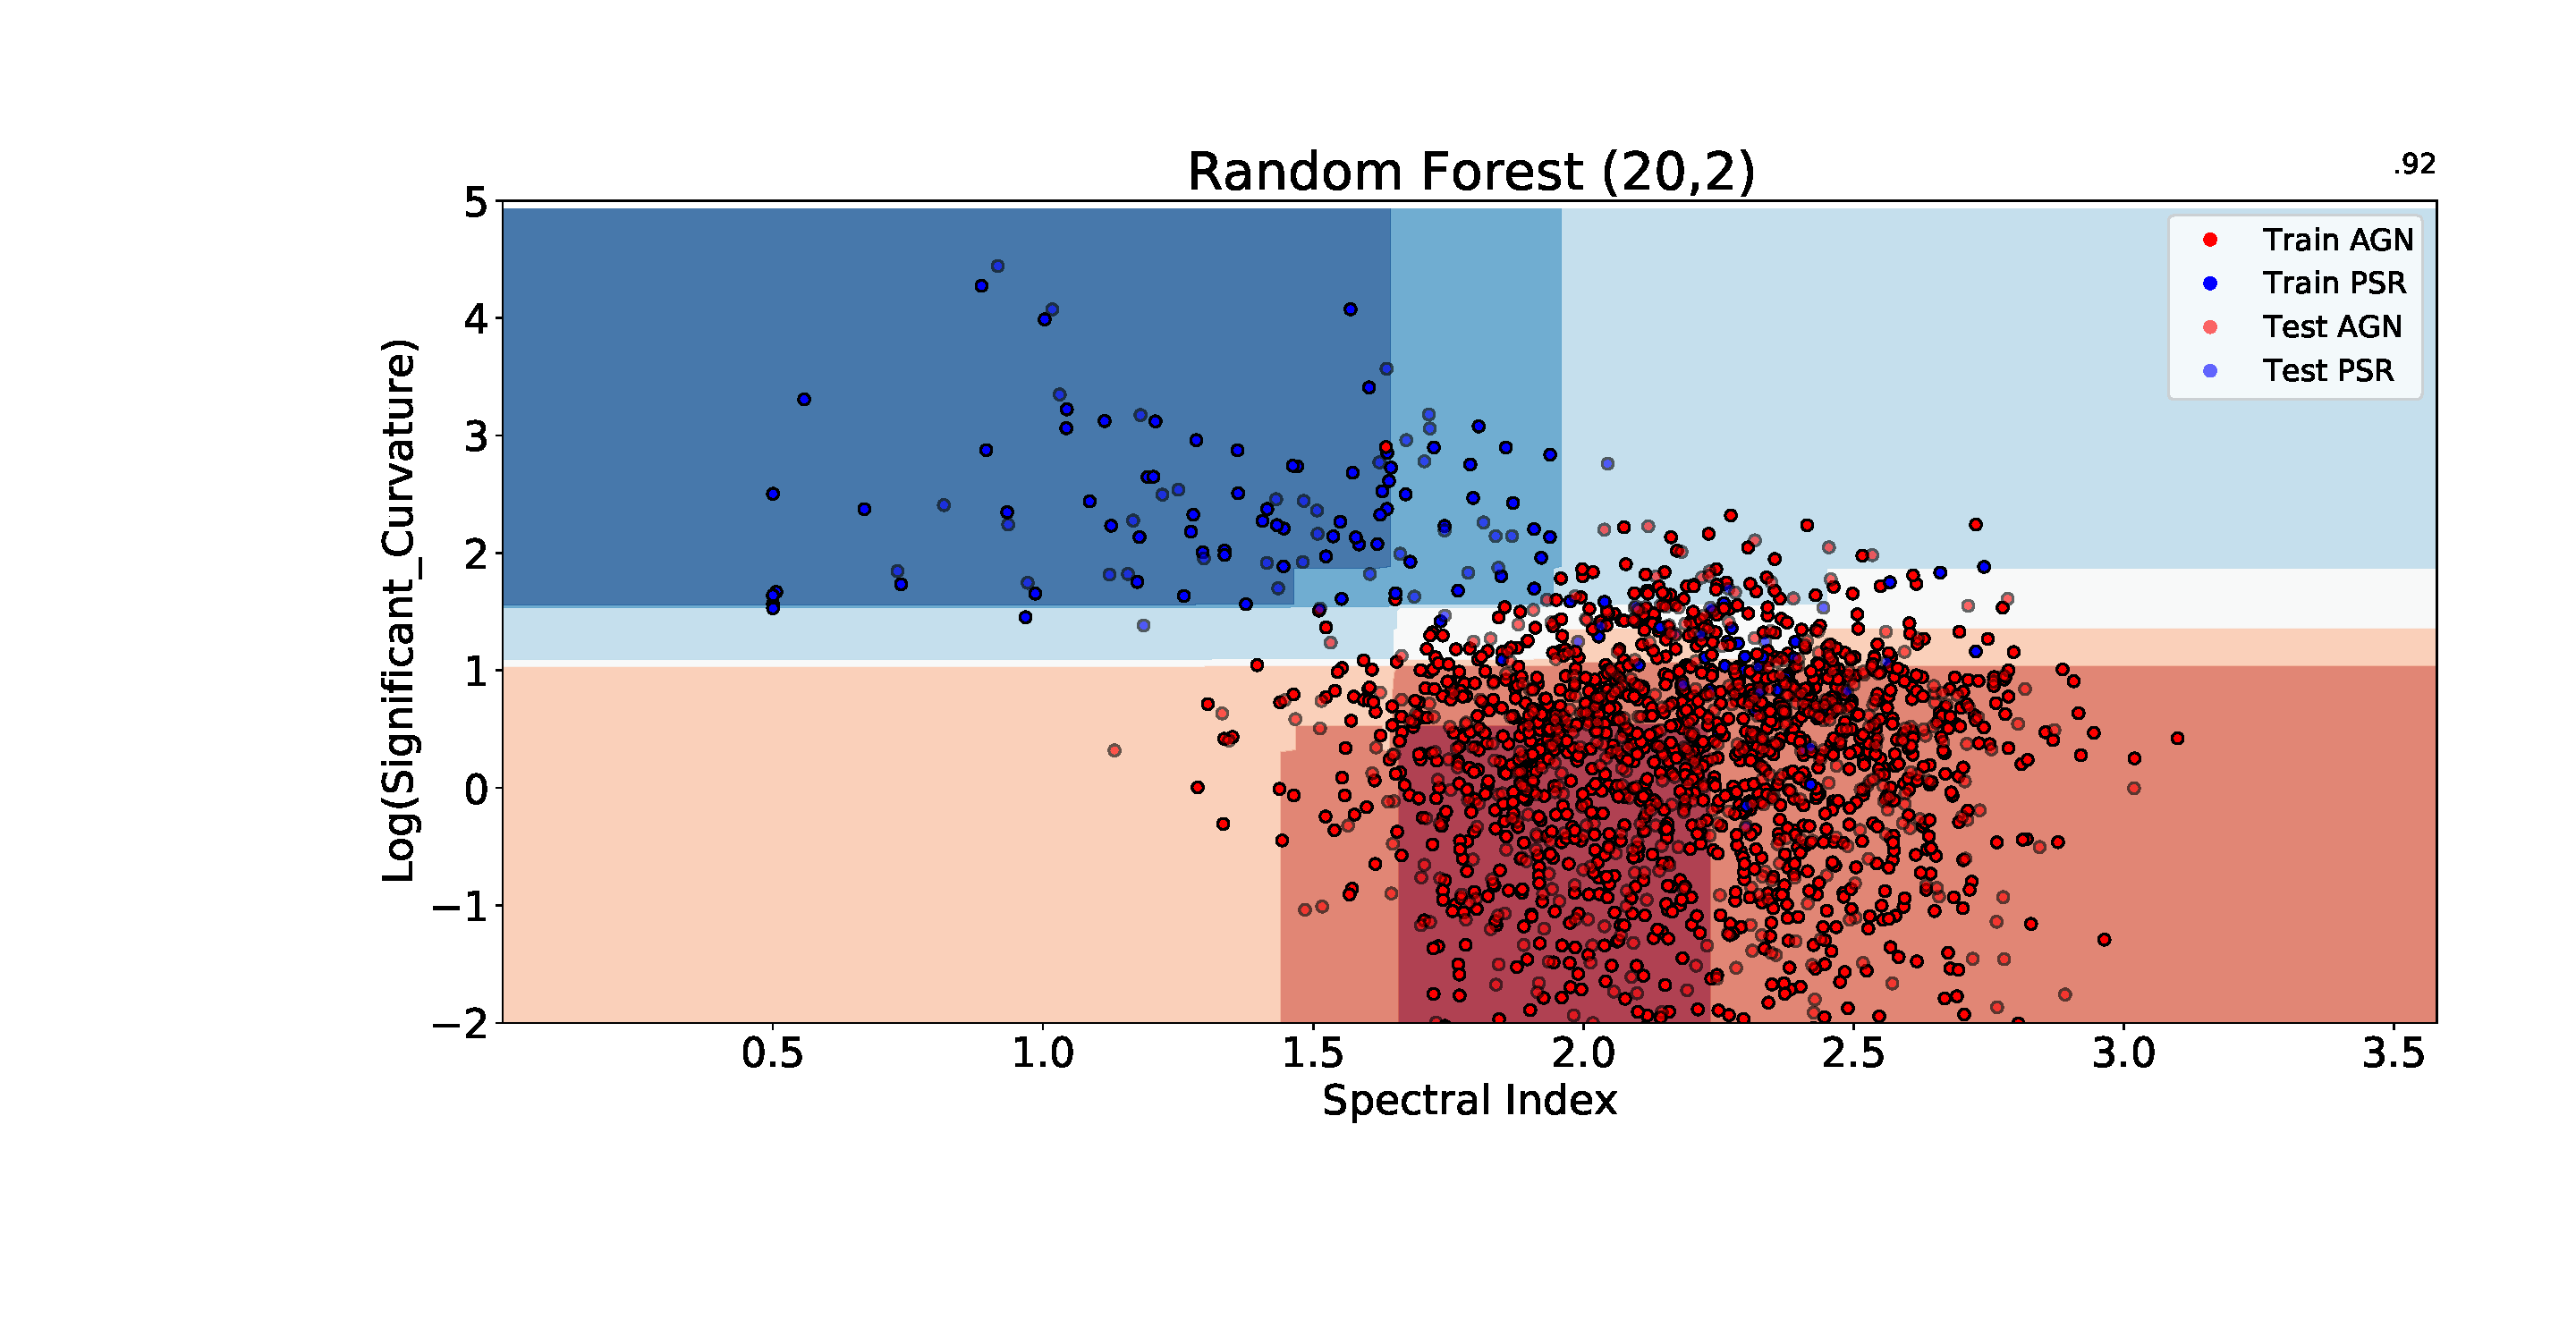
\includegraphics[width=\twocolumnwidth\textwidth]{plots/classification_domains/rf_20_2.pdf}
%>>>>>>> a522eecb66fa0cf6f440bc2907db2c42d74cac67
%\caption{Classification Domains of RF.  \dima{Why don't we show the domains for the final model, which we use for predictions?
%Moreover, it looks like for max depth 12 the model overfits the data, i.e., using max depth of 4 or 5 would be better for the final model.
%We should also add color bars for all domain plots and make the labels larger.}}
%\label{fig:RF_domains}
%\end{figure*}




\subsection{Boosted Decision Trees}

The hyper-parameters for BDT algorithms are similar to RF algorithms: they are the number of trees and the maximal depth.
We used the gradient boosting algorithm for the construction of BDT.
The classification is performed by a weighted average of trees, where the trees are constructed recursively in order to better address 
misclassifications from the previous step. 
%The new trees are added with an additional parameter $\nu$ called learning rate. 
%The learning rate itself is not a significant parameter, and we stuck with the default value.
%\dima{I'm not sure we need to discuss the learning rate, since we haven't done so in, e.g., neural networks}
Dependence of the accuracy on tree depth is shown in Figure \ref{fig:BDT_depth}. 
Firstly, unlike the RF, which is also an ensemble based method, the accuracy drops with an increase in the maximal depth above 2. Secondly, similar to RF, the number of trees is not significant above a threshold, which is $\sim$ 50 in the case of BDTs.
%\dima{Which depth do we use for the final algorithm, it looks like depth 2 gives the best results. What about depth = 1?}

\begin{figure}[h]
%\centerin
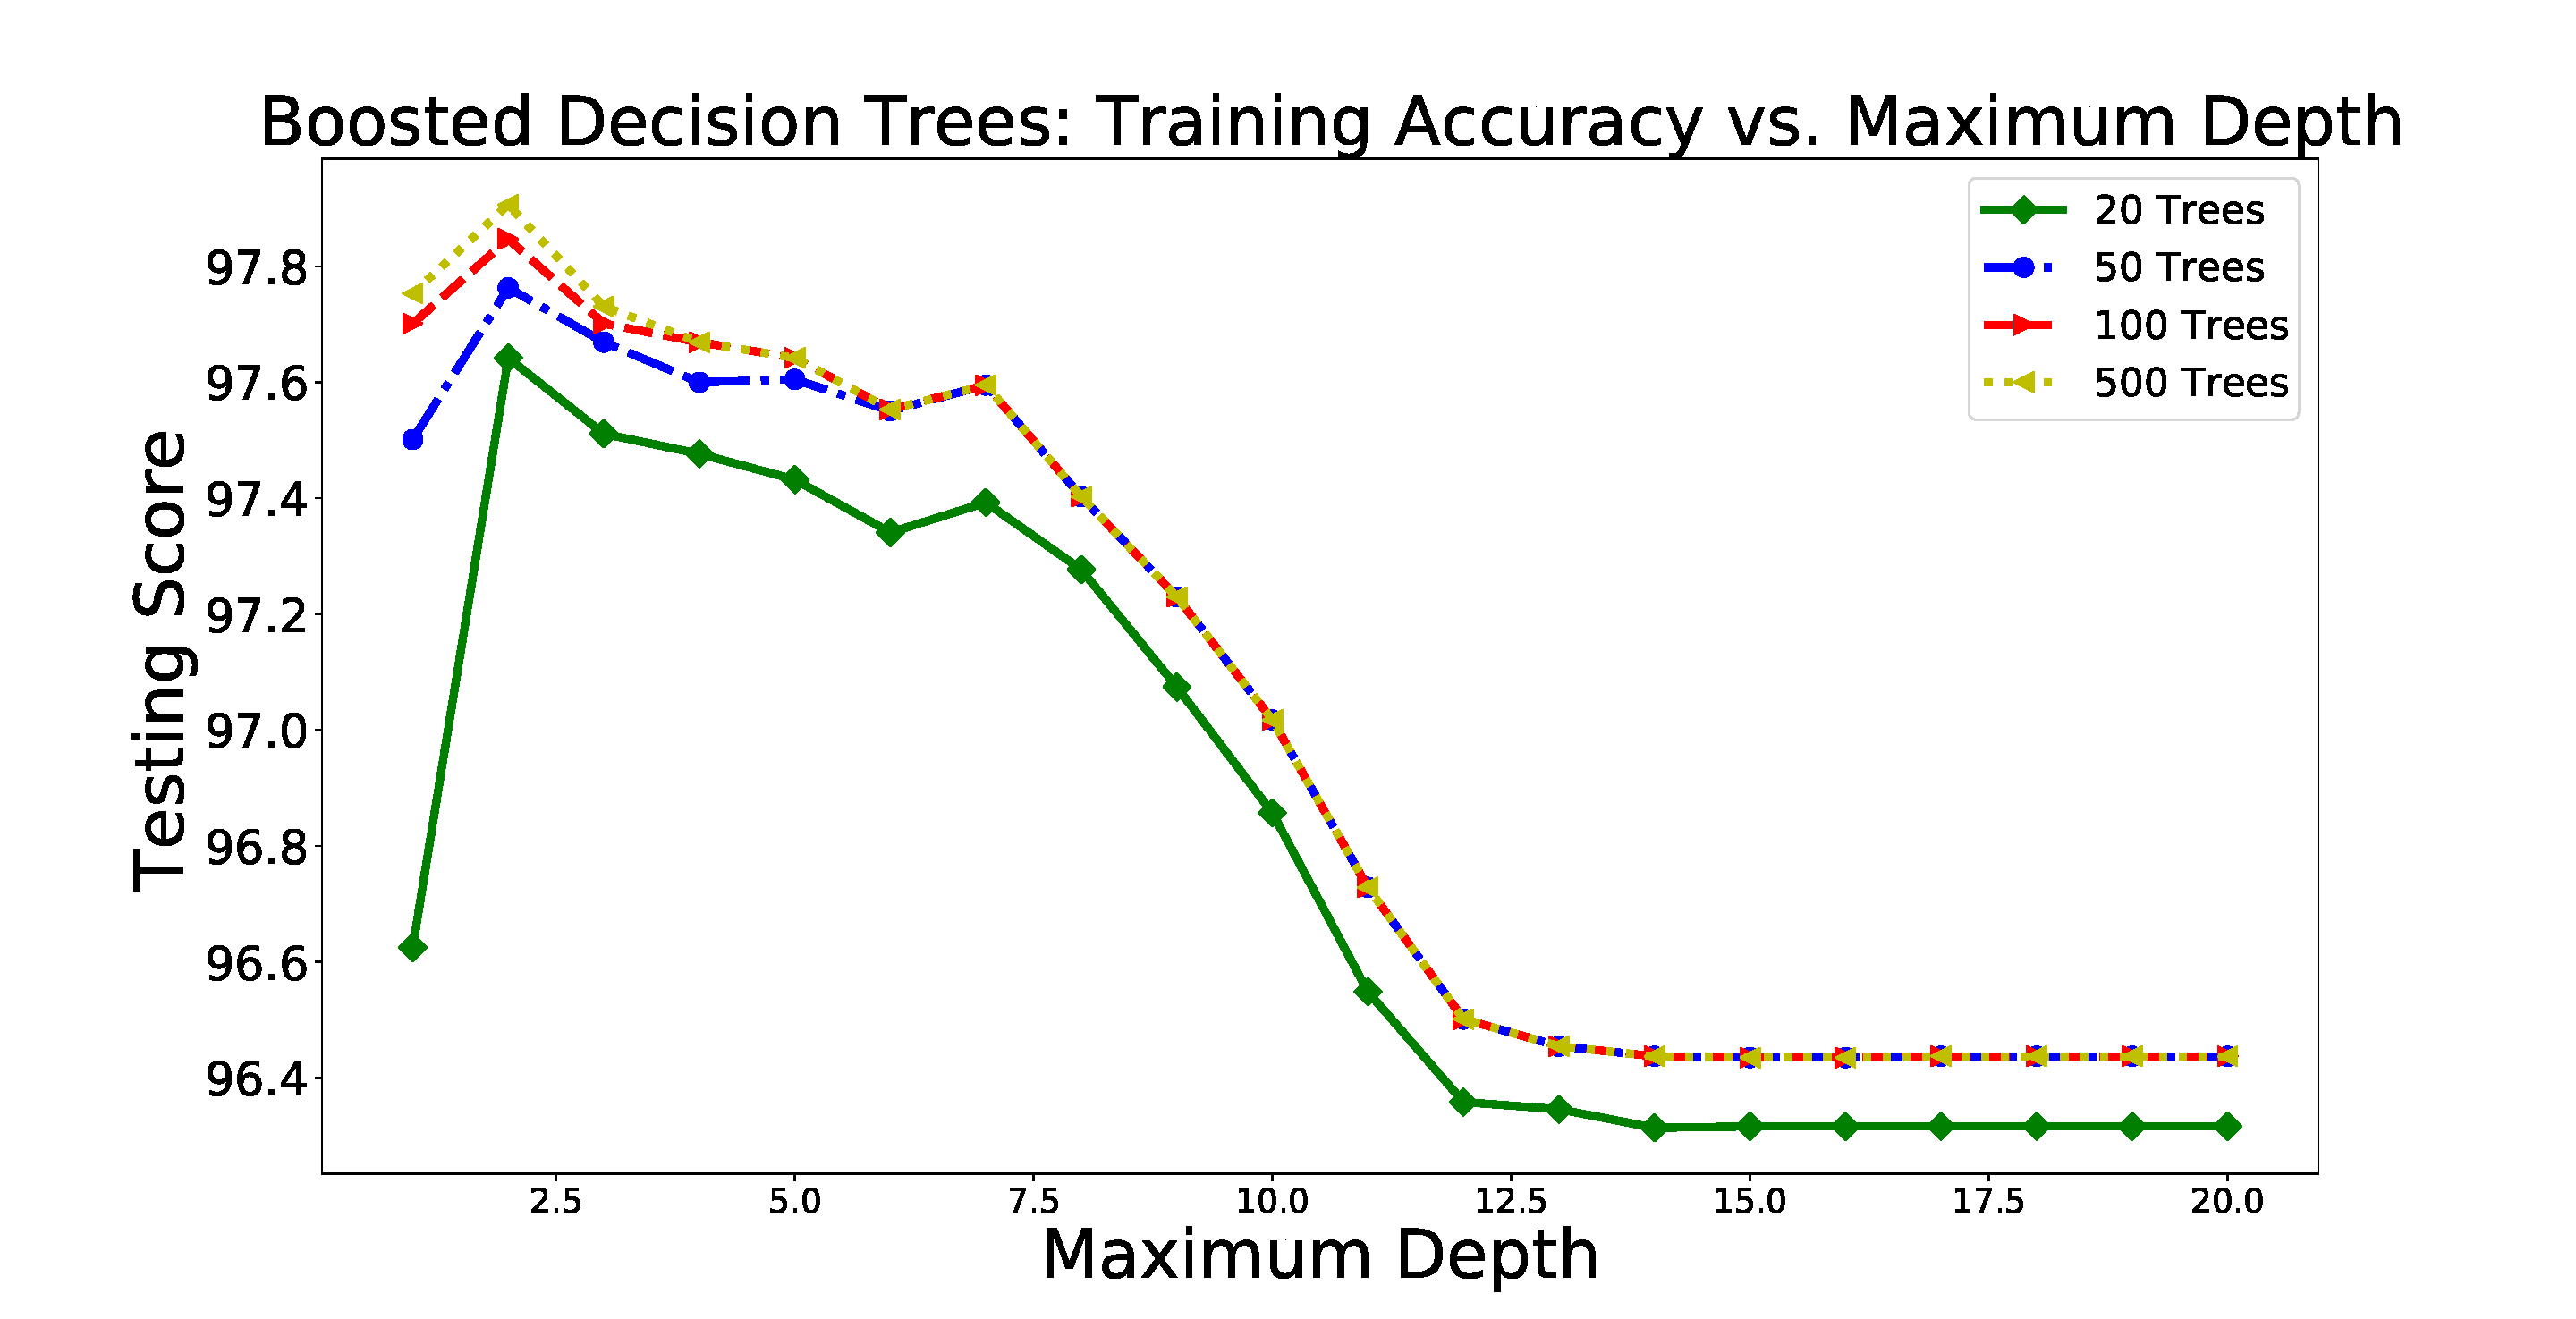
\includegraphics[width=\twopicsp\textwidth]{plots/bdt_train.pdf}
%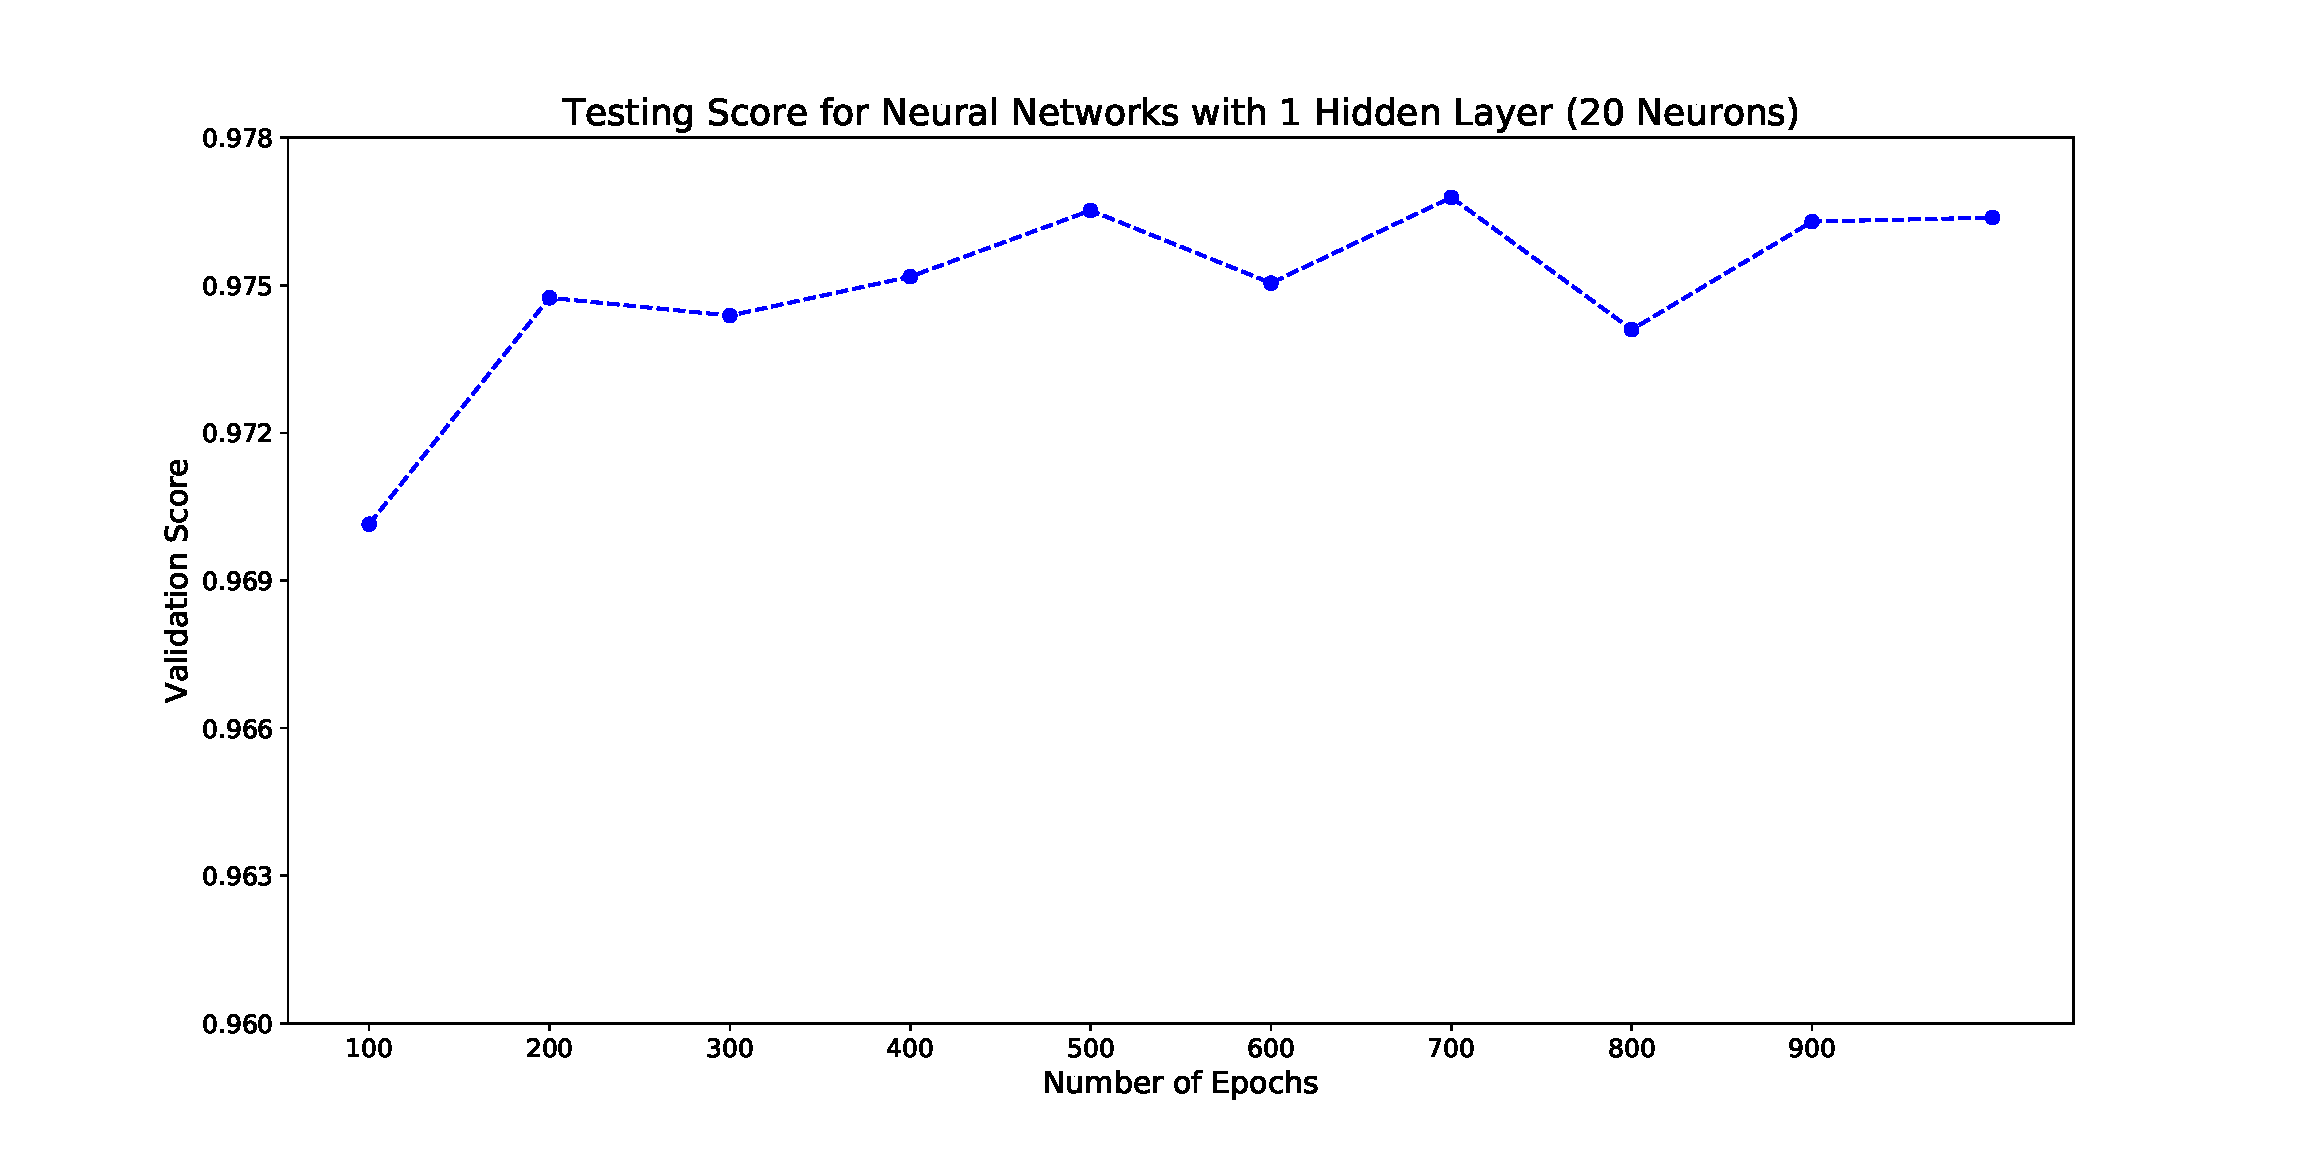
\includegraphics[width=\twopicsp\textwidth]{plots/epochsvsscore2_10seeds.pdf}
\caption{Dependence of BDT accuracy on maximum depth and the numbers of trees.}
\label{fig:BDT_depth}
\end{figure}

The classification domains in case of two features for the maximal depth of 2 and 12 are presented in Figure \ref{fig:BDT_domains}. 
It is interesting to note that already for the maximal depth of 2, the domains show a sign of overfitting: narrow bands in the class probabilities.
%The greater than a percent decrease in the accuracy from a max depth of 3 to a max depth of 15 can be explained by the domains, where we see a pattern of almost over-fitting the data. While for 2 features the decrease is small, it should increase as we increase the number of features, with a lower complexity network being enough for a good accuracy.
%Boosted Decision Trees again show a similar effect as Random forests in their classification, and have a significant difference when the model complexity is changed.

\begin{figure}[h]
%\centerin
\hspace*{-1cm}
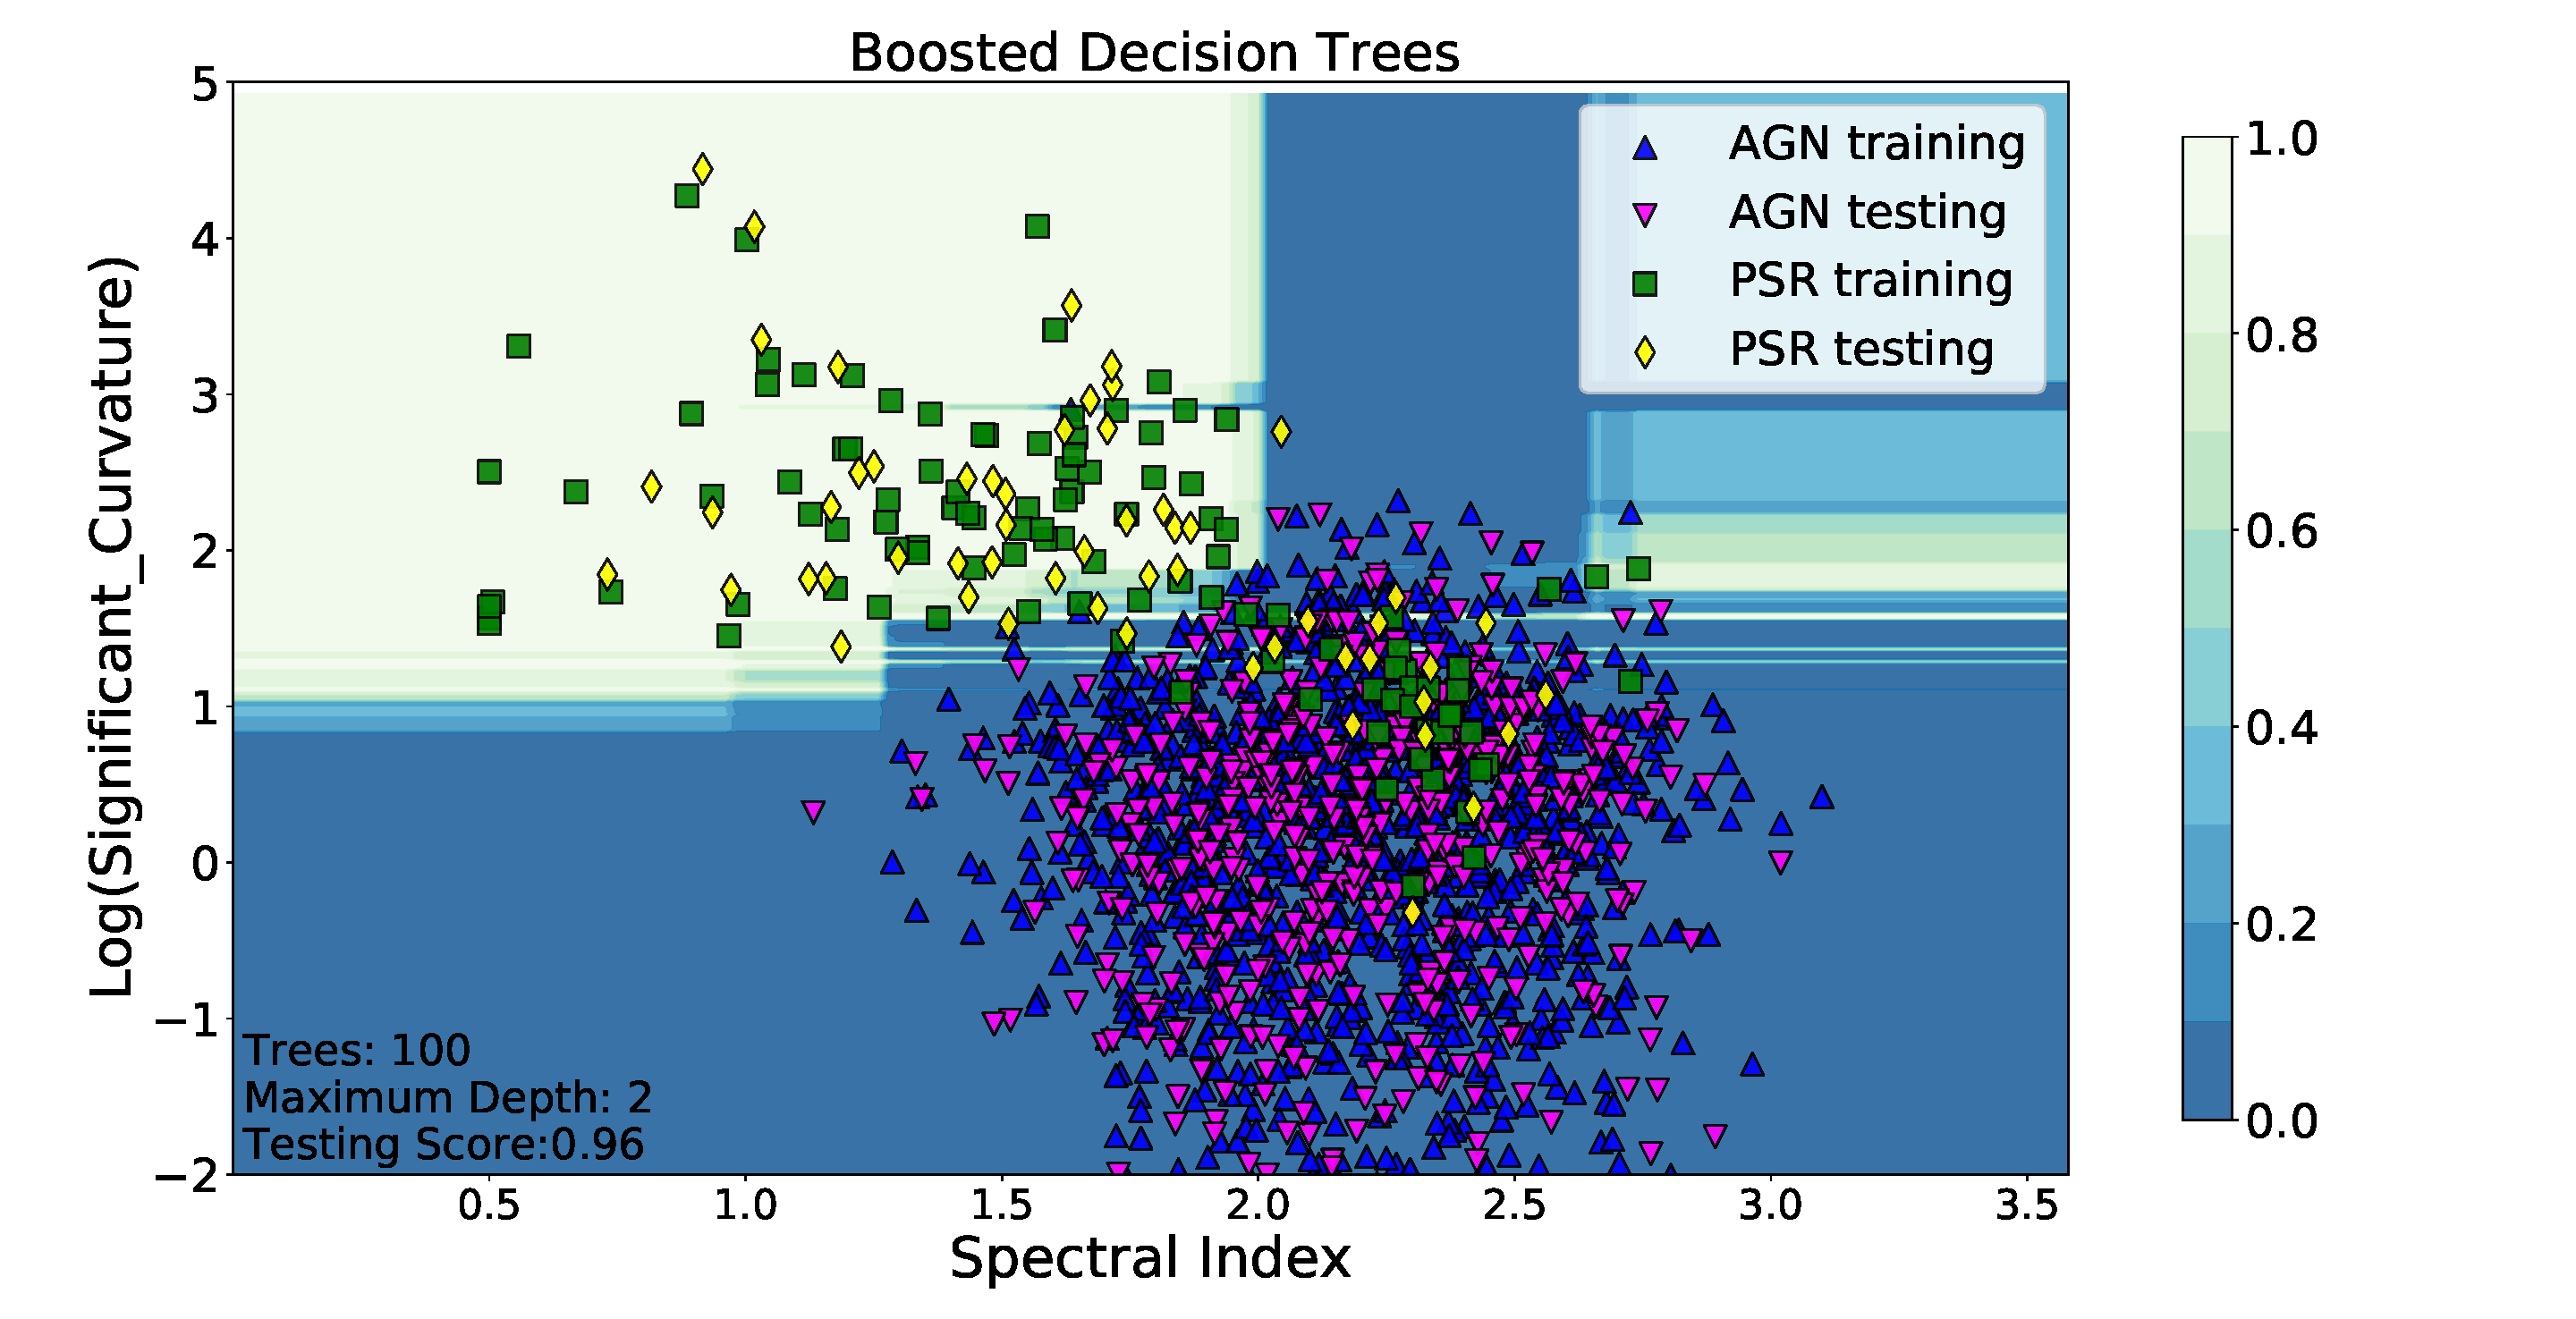
\includegraphics[width=0.5\textwidth]{plots/bdt_100_2.pdf}
\hspace*{-1cm}
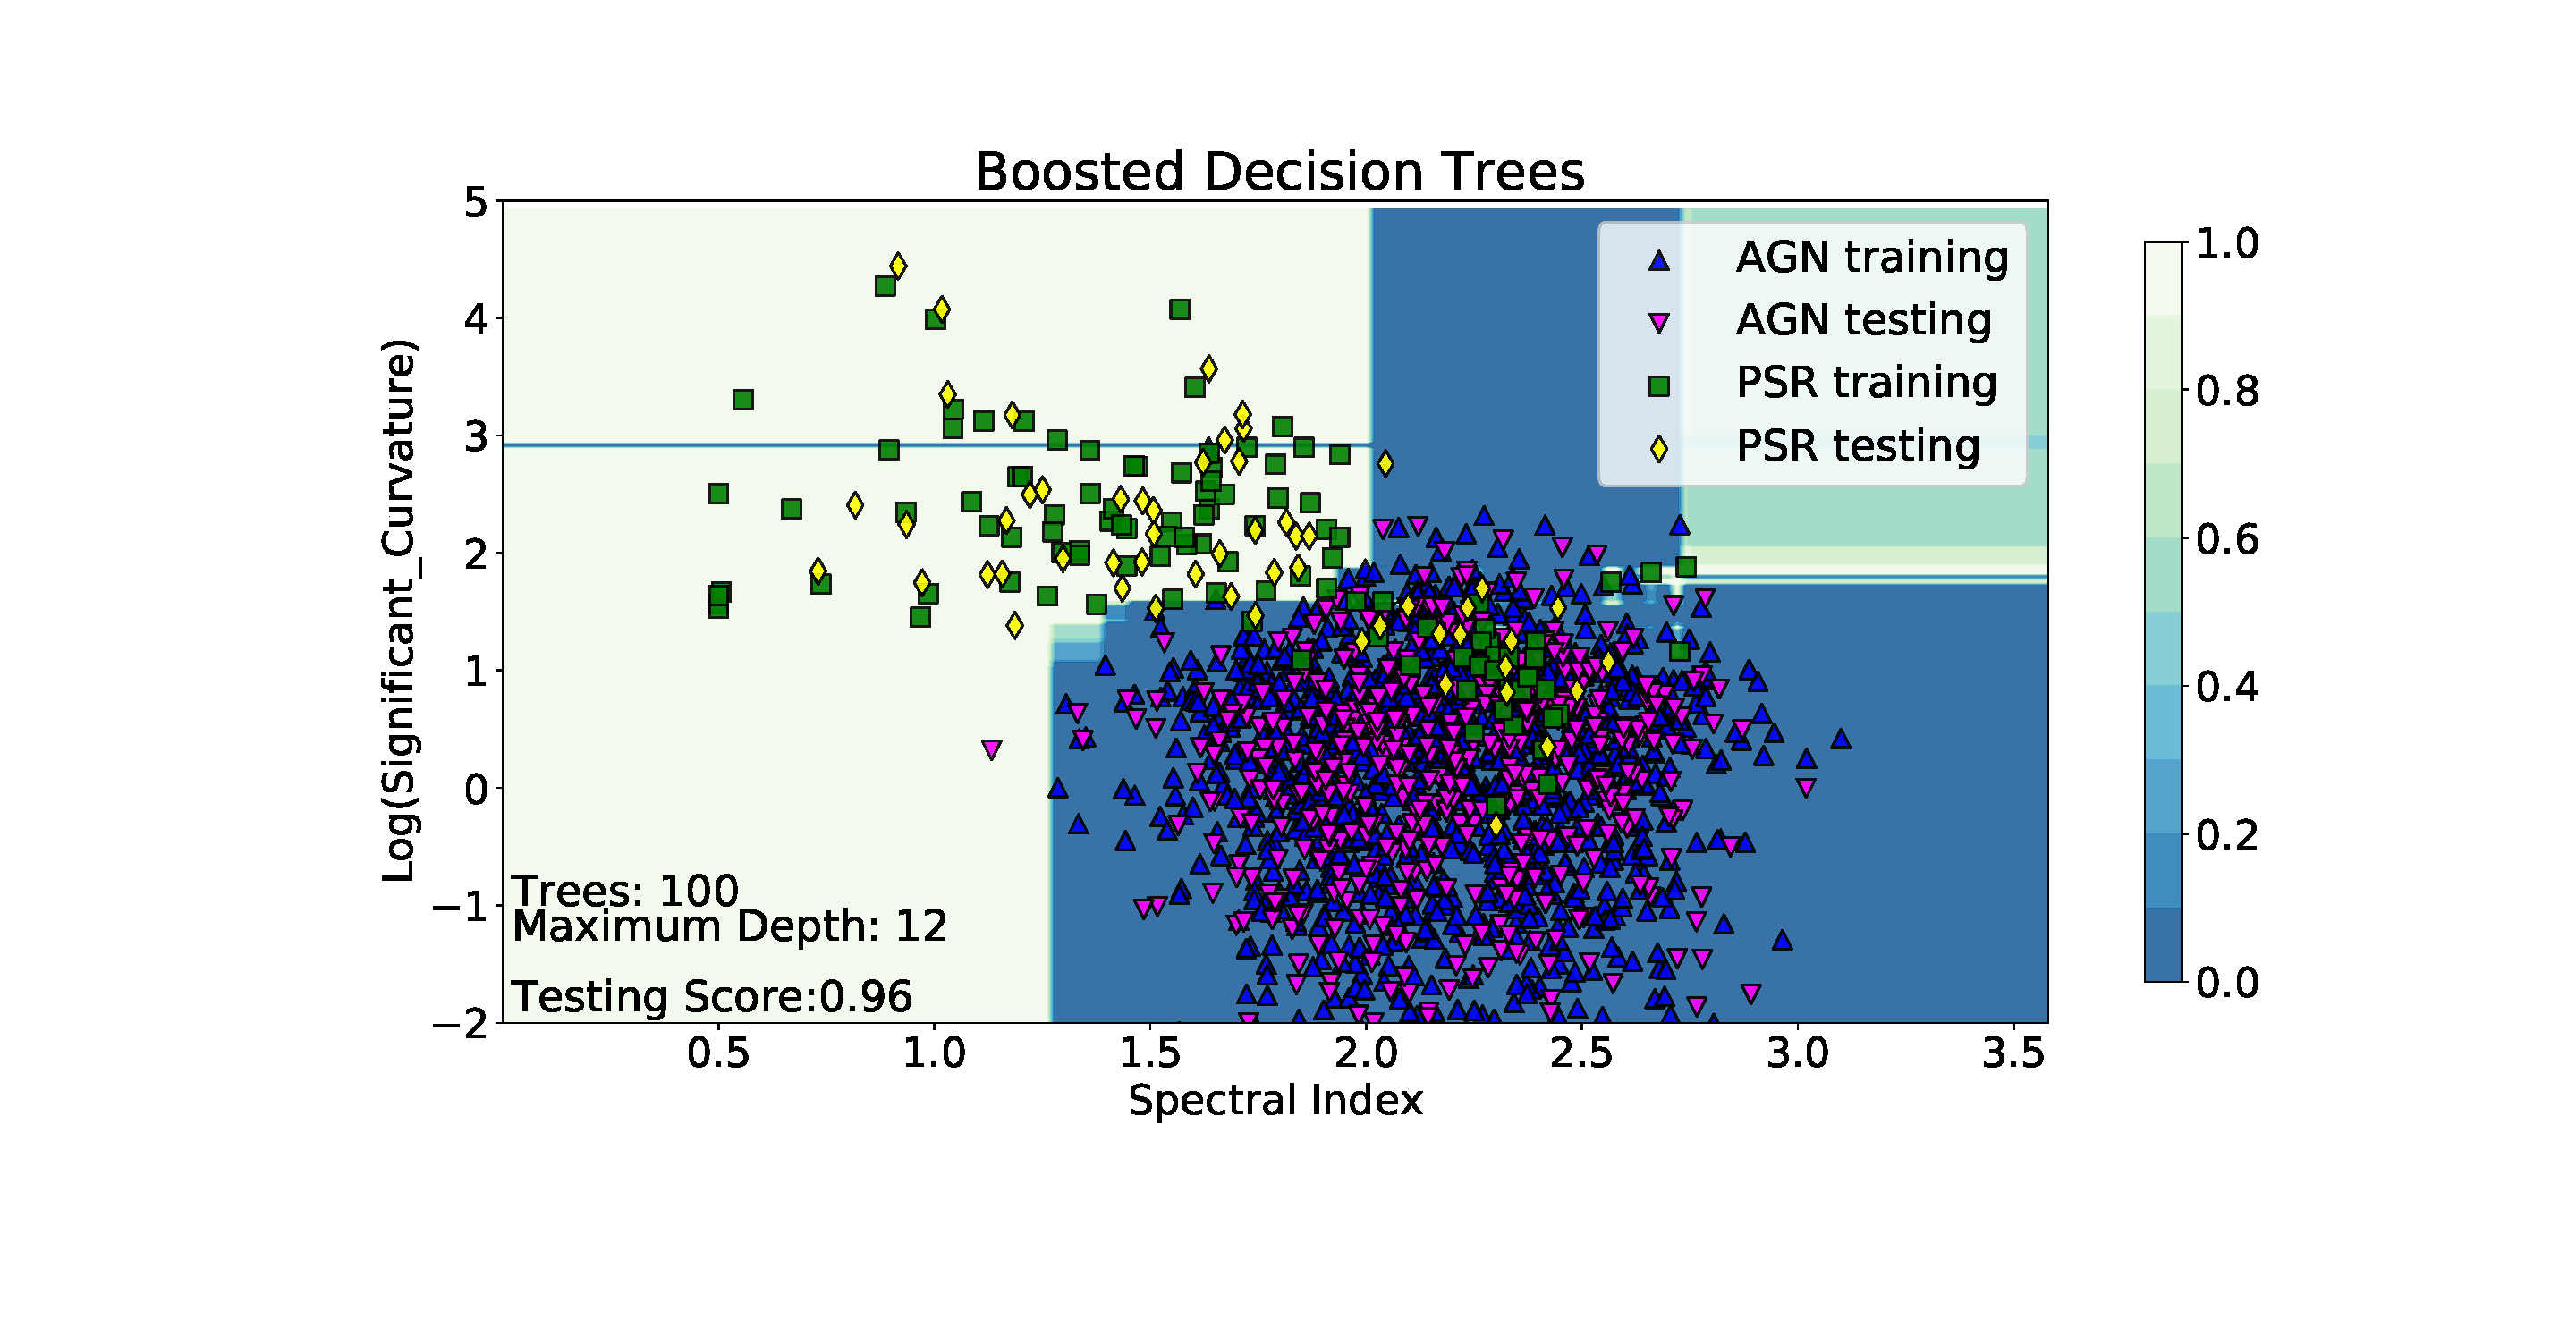
\includegraphics[width=0.5\textwidth]{plots/bdt_100_12.pdf}
\caption{Classification Domains for BDT.}
\label{fig:BDT_domains}
\end{figure}


\begin{comment}
Is learning rate equivalent to the 
Boosted Decision Trees or Gradient boosting algorithms are similar to Random Forests, having number of trees and maximum depth as parameters. However, here we also have the learning rate which specifies how fast (or slow) a model learns. This parameter is quite important, as a high value will converge faster but under-fit, whereas a lower value will over-fit. Therefore, we first chose an architecture of (50,6) and (20,6) to look at the dependence on number of trees. Here we found that low learning rate is preferred, and the maximum accuracy is reached at around 0.1-0.3. After a maximum the accuracy falls drastically since the BDT doesn't have enough time to learn properly. However, after a certain maximum depth, this doesn't hold true anymore irrespective of the number of trees. In this case, the BDT is complex enough that it learns fast and the accuracy doesn't fall even for higher learning rates. The figures below illustrate this.\\



\begin{figure}[h]
%\centerin
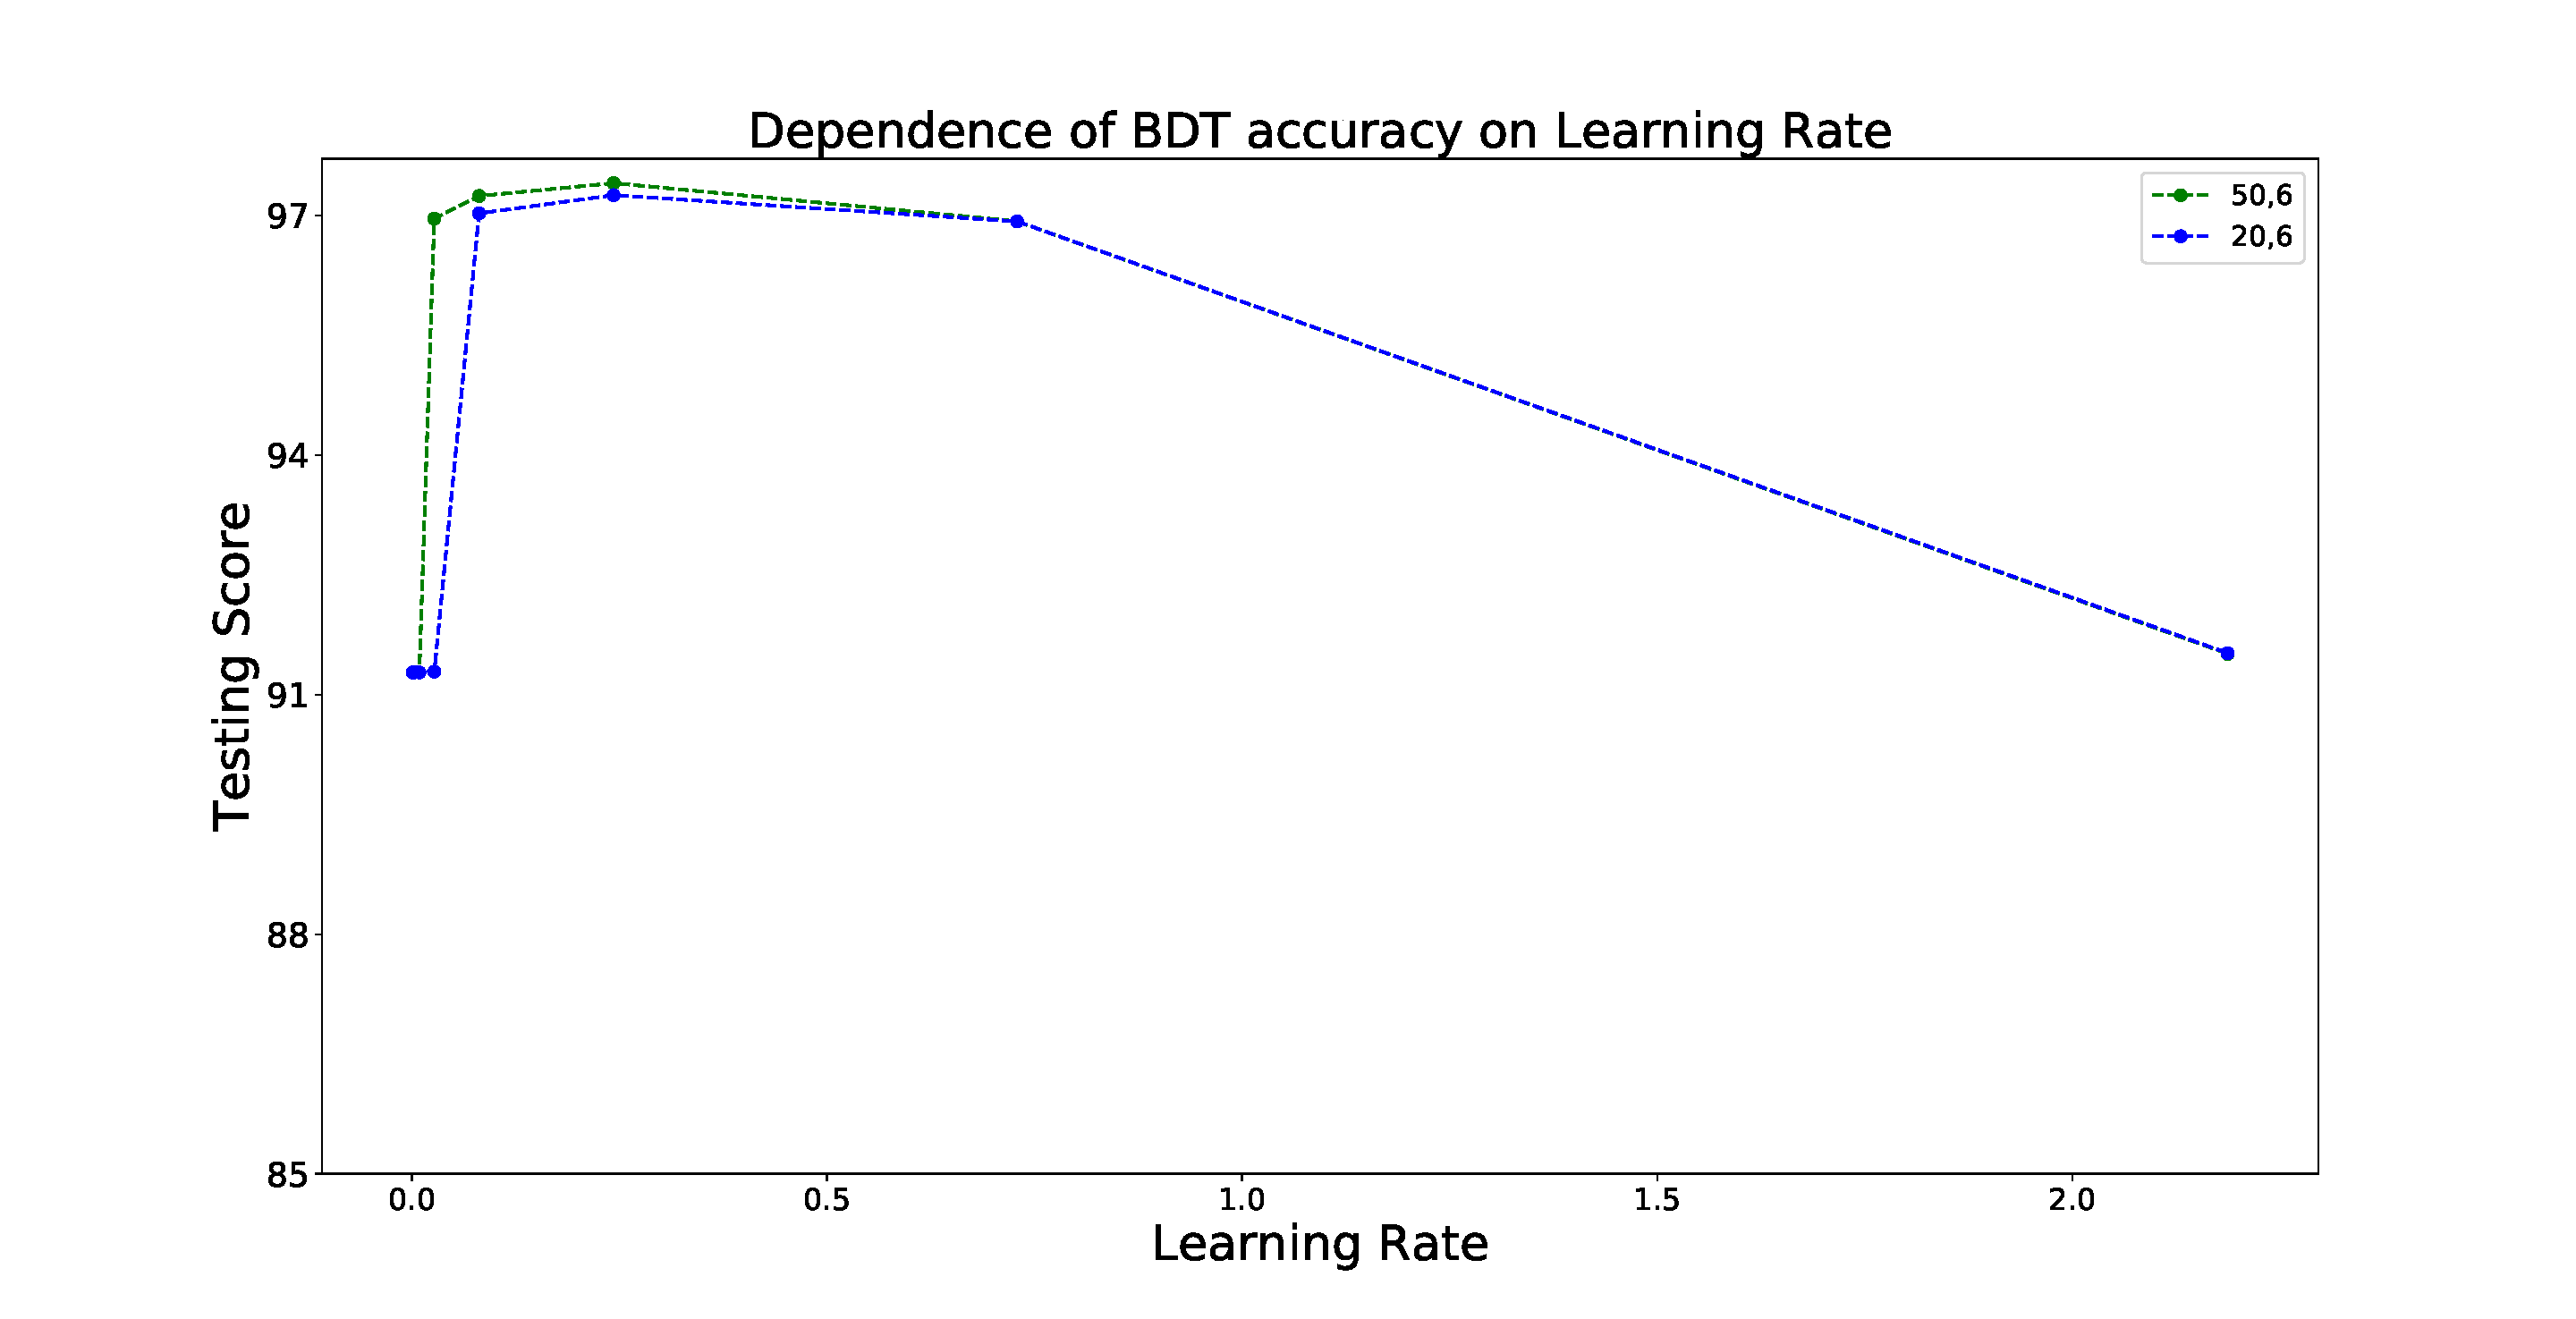
\includegraphics[width=\twopicsp\textwidth]{plots/lr.pdf}
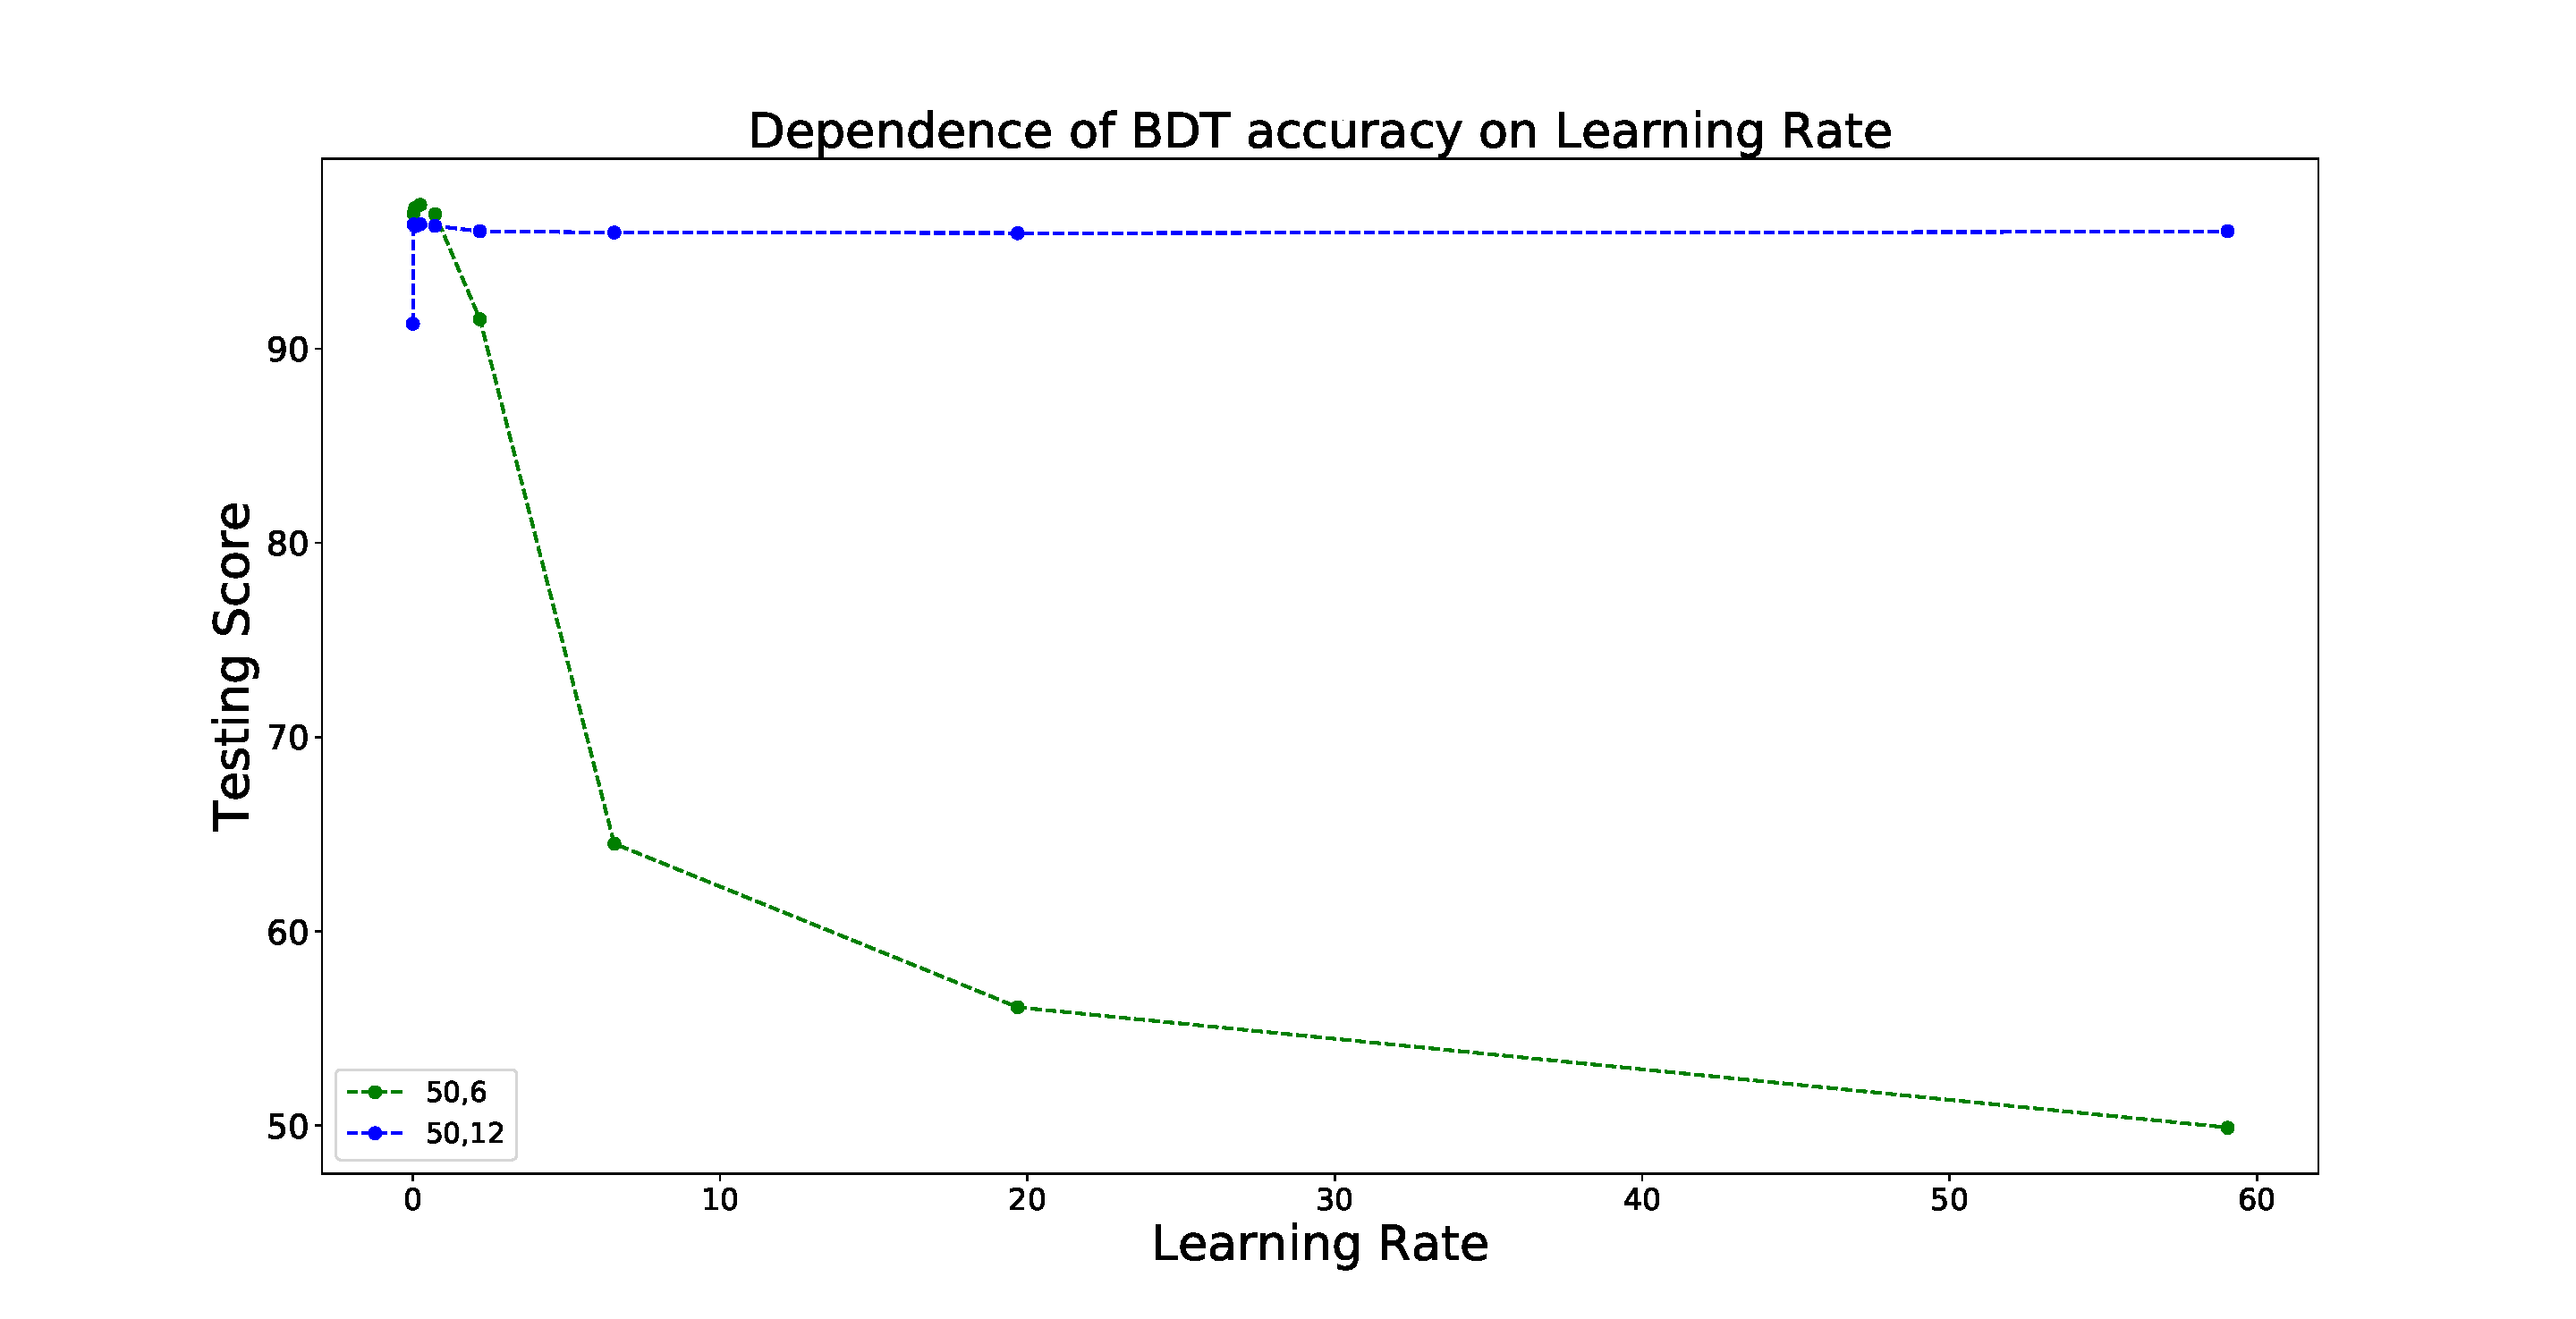
\includegraphics[width=\twopicsp\textwidth]{plots/lr3.pdf}
\caption{Dependence of BDT accuracy on learning rate with number of trees and maximum depth kept constant.
\dima{I'd include the name of the algorithm in the filenames, so that we can easier find them in the folder. ``lr'' sounds more like logistic regression.}}
\label{fig:BDT_learning_rate}
\end{figure}
\end{comment}





\subsubsection{Neural Networks}

In the case of NN, the number of free parameters depends on the number of hidden layers and on the number of neurons in the hidden layers. The final model accuracy also depends on the number of epochs that the network is allowed to be trained for and on the optimization algorithm. 

\begin{figure}[h]
\centering
\hspace*{-0.5cm}
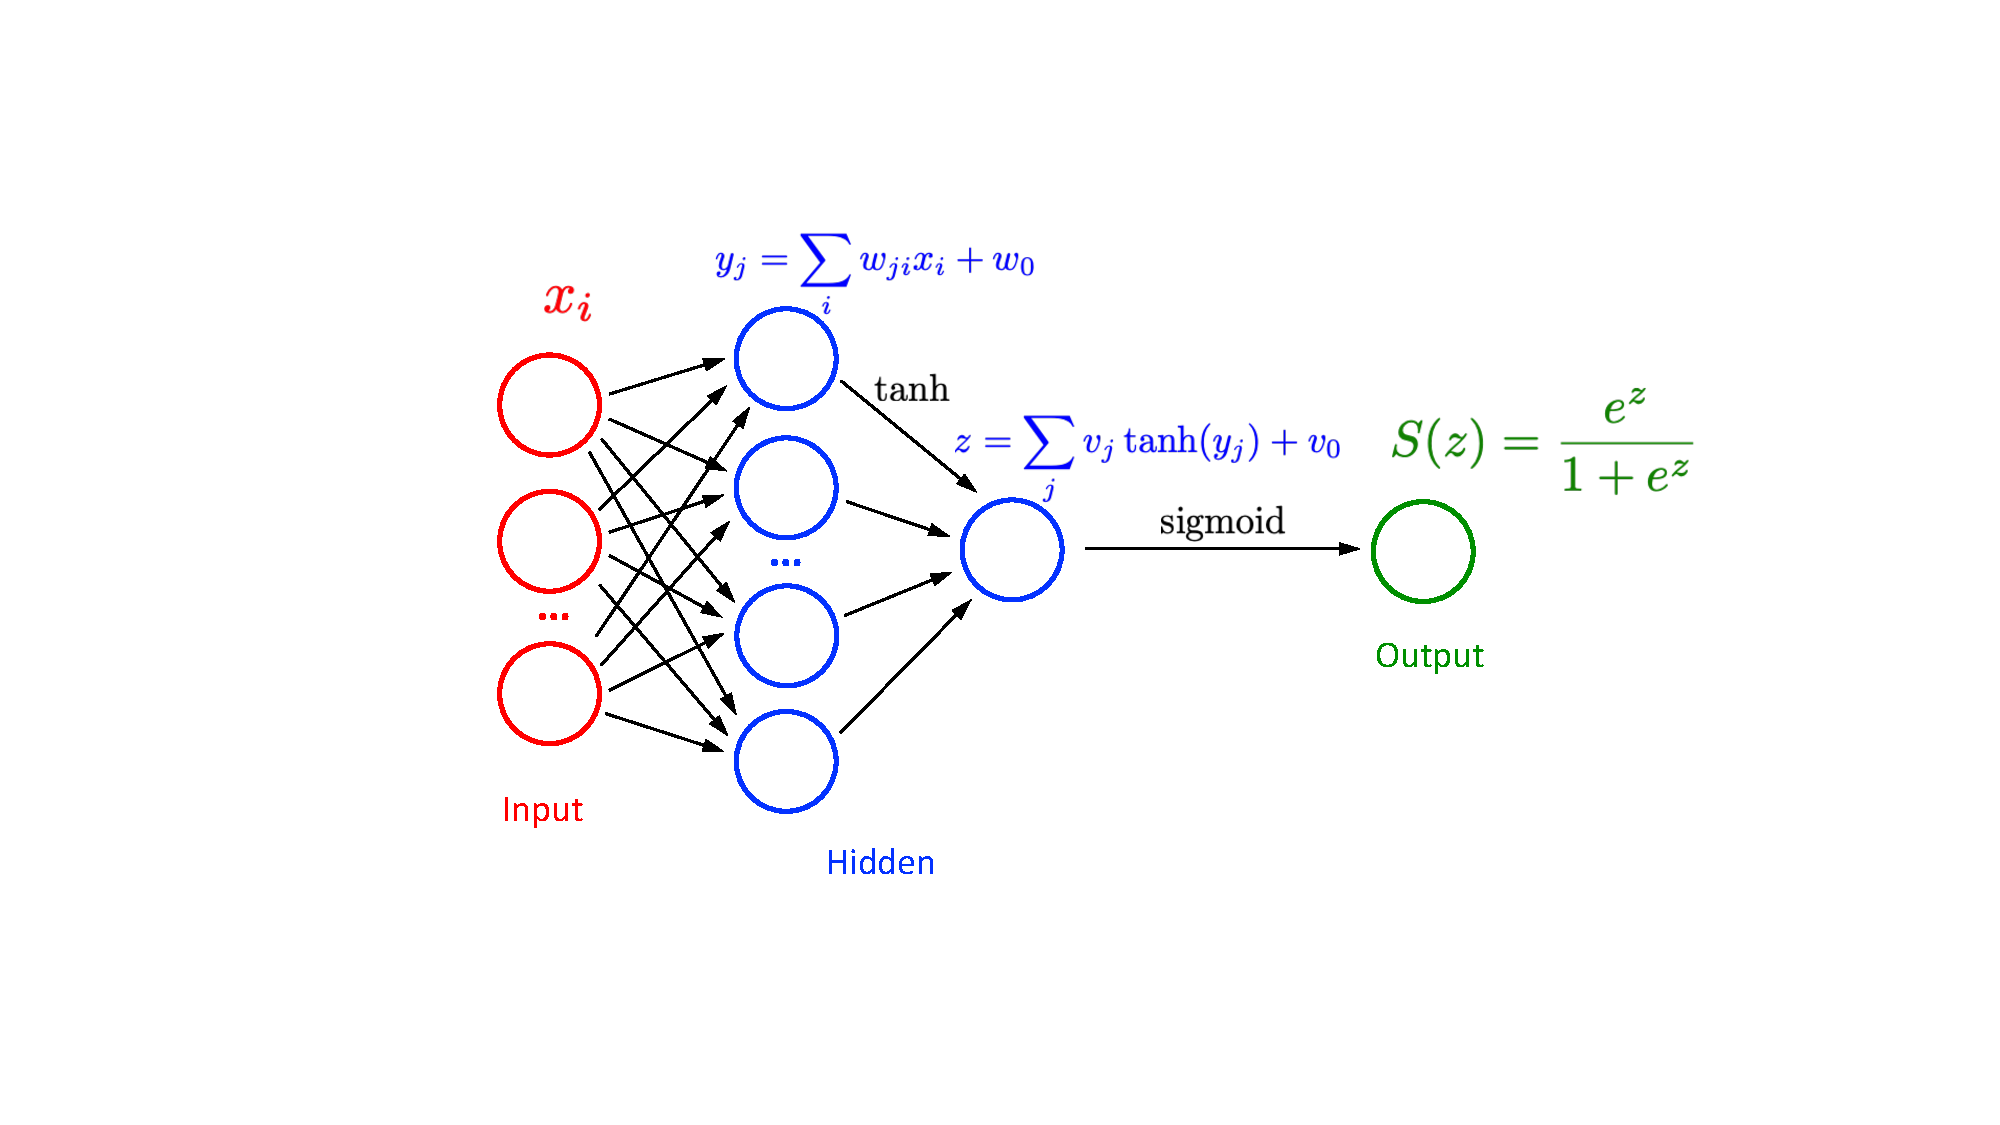
\includegraphics[width=0.45\textwidth]{plots/CNN_network.pdf}
\caption{
NN architecture.
}
\label{fig:NN_structure}
\end{figure}

The general architecture of the NN that we use in this paper is shown in Figure \ref{fig:NN_structure}.
It is a fully connected NN with 10 input nodes (shown by red circles with input features $x_i$), two hidden layers (shown by blue circles),
and an output layer (shown by the green circle).
The first hidden layer consists of several nodes with values $y_j$. For the activation function between the first and the second hidden layers we use either hyperbolic tangent (tanh - shown on the plot) or rectified linear unit (relu).
The activation function between the second hidden layer and the output node is sigmoid, which we use to make sure that the output value can be interpreted as a class probability.
The unknown parameters are weights of the input features and the output of the first hidden layer, $w_{ji}$ and $v_j$ respectively,
and offsets $w_0$ and $v_0$.
The unknown parameters are optimized by minimizing the loss function. The loss function used is the log loss, defined as: $-\text{log}(\frac{y_t}{y_p})=-(y_t\text{log}(y_p)+(1-y_t)\text{log}(1-y_p))$, where $y_t$ are the true labels and $y_p$ are the predicted values.
We have also tried to use three hidden layers with several nodes in the first two hidden layers and one node in the third hidden layer.
The accuracy was similar to the networks with two hidden layers. Consequently, we have chosen to use a simpler model with two hidden layers.

\begin{figure}[h]
%\centerin
\hspace*{-0.5cm}
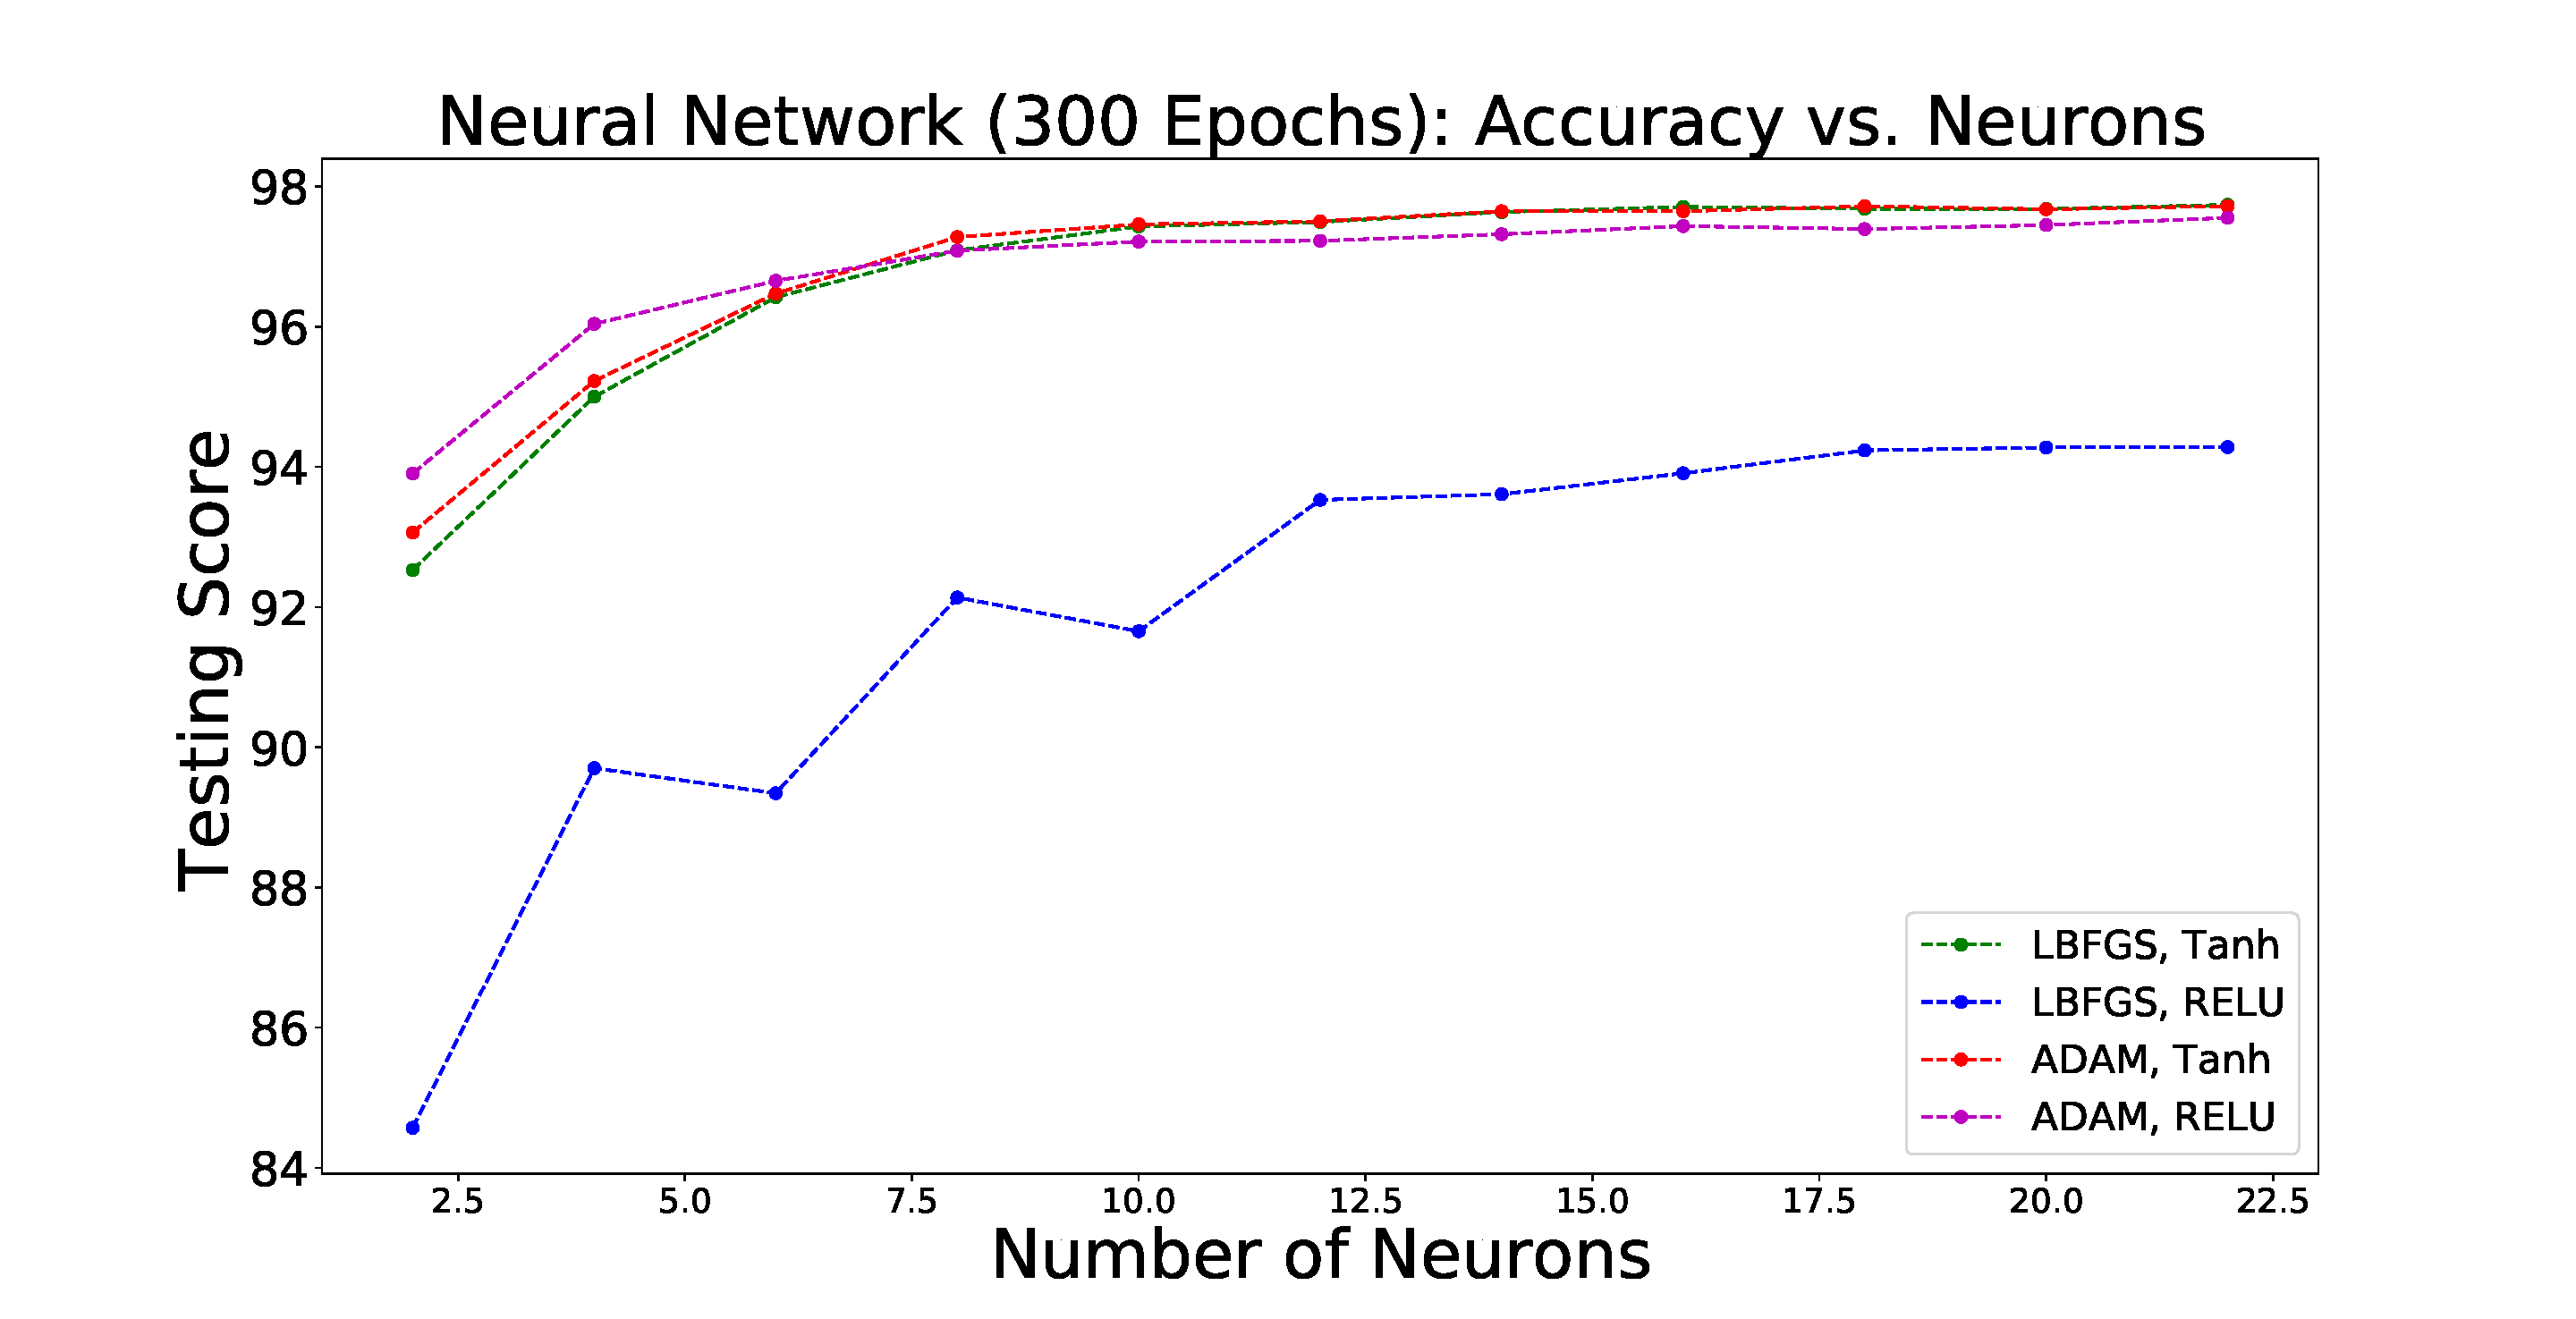
\includegraphics[width=0.5\textwidth]{plots/nn_neurons_300epochs.pdf}
%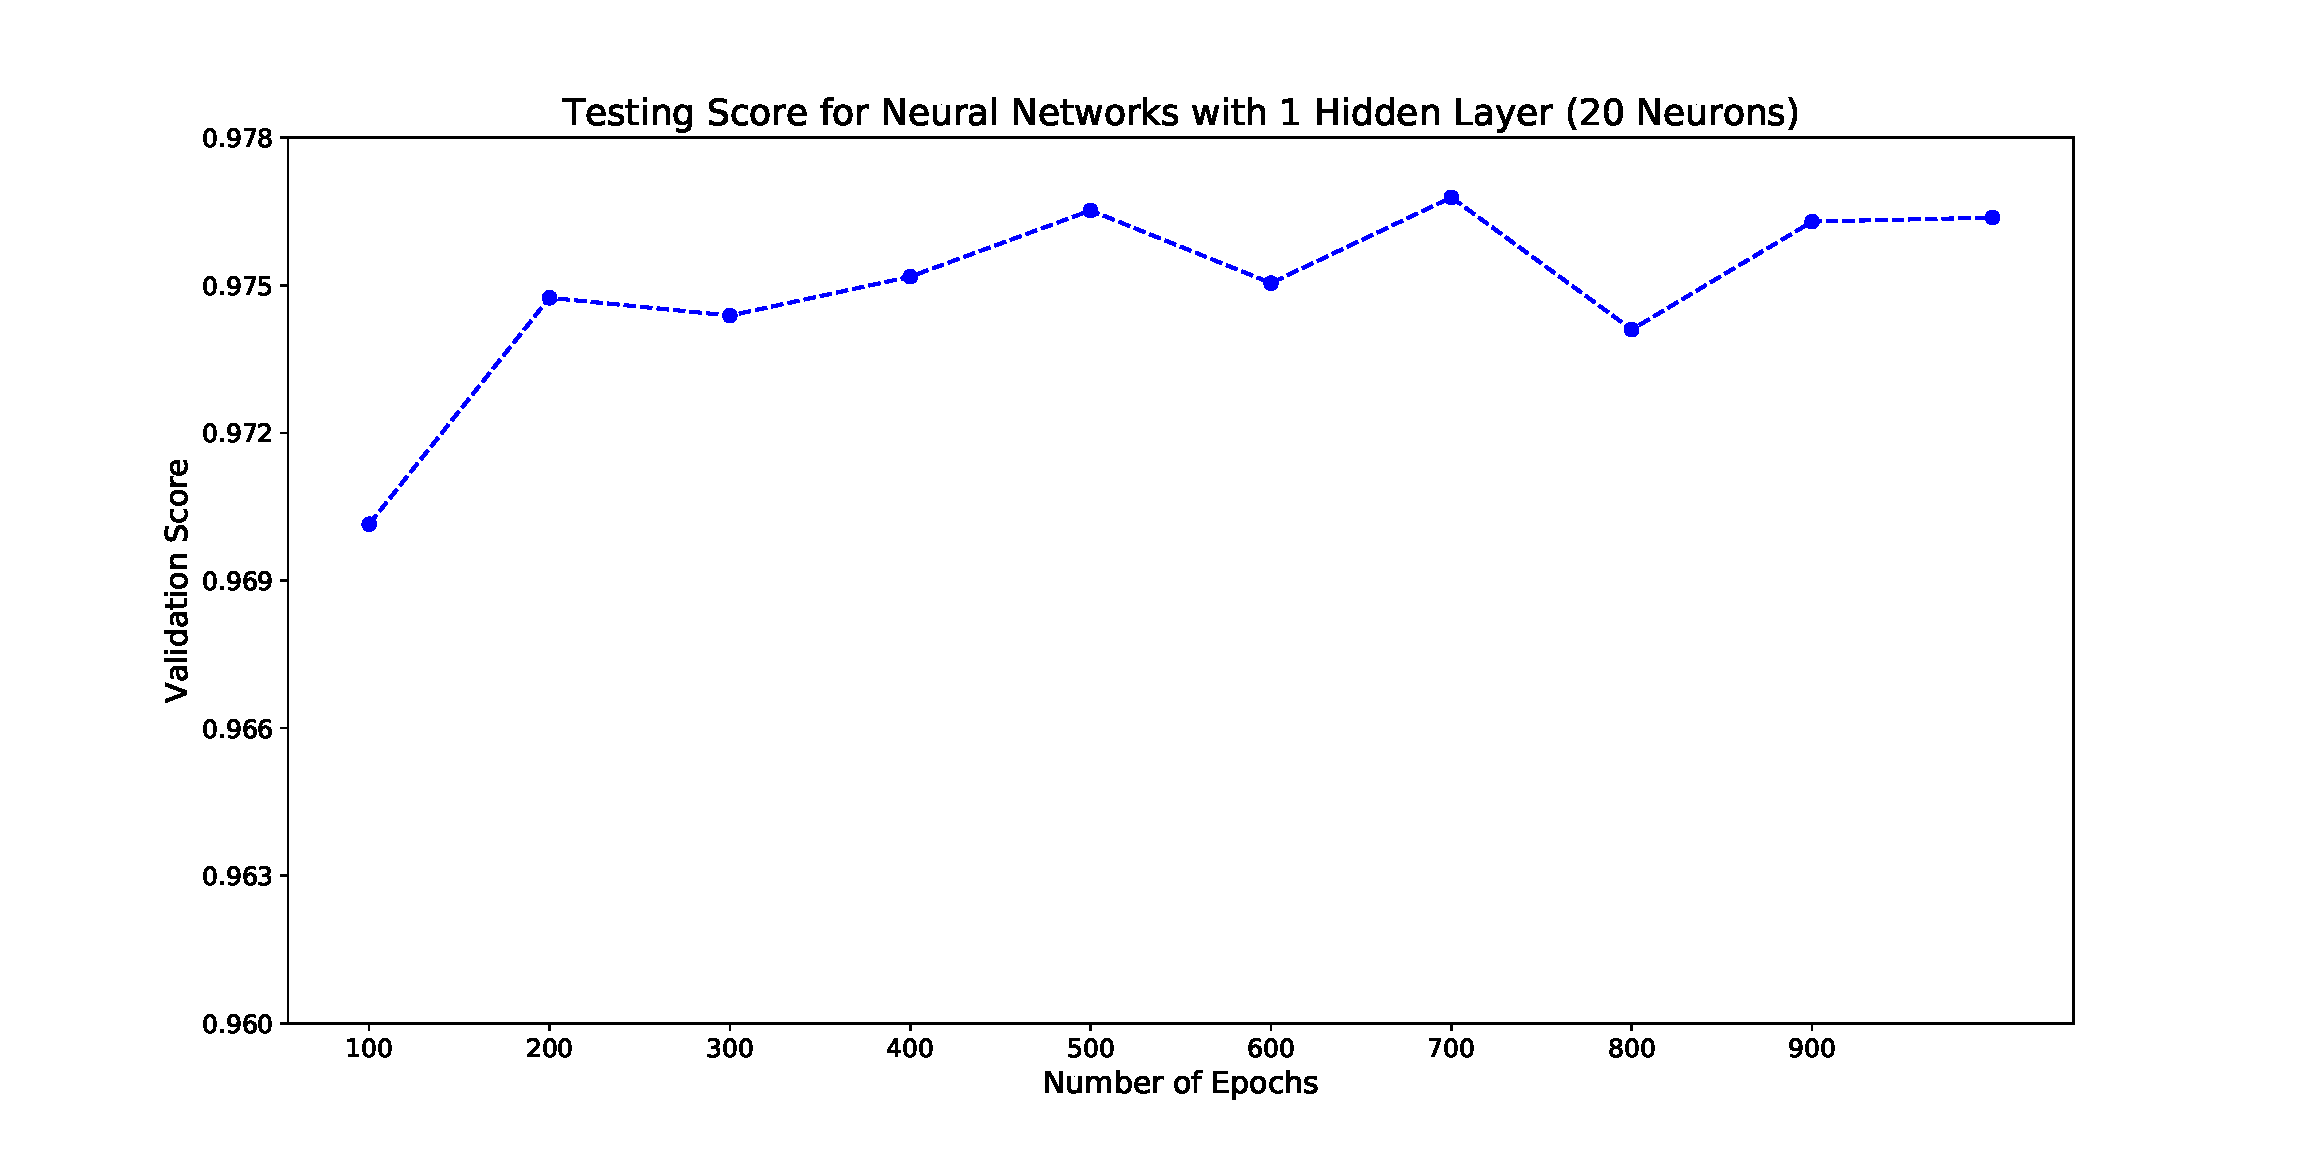
\includegraphics[width=\twopicsp\textwidth]{plots/epochsvsscore2_10seeds.pdf}
\caption{Dependence of accuracy on number of neurons for different models.}
%\dima{I'm not sure I understand where you use Tanh or RELU activations, if we have only one hidden layer with sigmoid activation (I guess) for classification?}}
\label{fig:NN_neurons}
\end{figure}

Dependence of the accuracy on the number of neurons in the hidden layer is shown in Figure \ref{fig:NN_neurons}. 
We compare two activation functions after the first hidden layer (tanh and relu) and two optimization algorithms: L-BFGS and ADAM. 
L-BFGS (Limited memory Broyden-Fletcher-Goldfarb-Shanno) is an approximation of the quasi-newtonian BFGS method. The BFGS method uses the full inverse of the Hessian matrix to find the direction of movement for minimizing the gradient. The limited memory counterpart however, only stores a smaller representation of the full matrix. This makes this method much faster for larger data-sets.
ADAM on the other hand belongs to a relatively newer family of algorithms which use gradient descent. Gradient descent is a first-order method to find the local minima or maxima of a differentiable function. Nowadays, this process is made more efficient by taking the gradient from parts of the data-set instead of the entire data-set itself. This is called stochastic gradient descent, since the data is selected randomly. ADAM is a newer approach of the stochastic family using adaptive network learning rates for every parameter. ADAM is usually preferred for Neural Networks with big data-sets. However since ADAM converges slower, a higher number of epochs is needed to reach the best accuracies.
10 neurons in the hidden layer appears to be an optimal choice, since increasing the number of neurons leads to no significant increase in accuracy for all models. 
We find that tanh is a better activation function in our case, as it provided a good result for both optimization methods, whereas relu is good only in the case of ADAM optimizer.
%As a method of choice we will use in the following 10 neurons in the hidden layer with tanh activation function and ADAM optimizer.
In Figure \ref{fig:NN_neurons} we use 300 epochs for training.
Dependence on the number of epochs (number of iterations in fitting) is presented in Figure \ref{fig:NN_epochs}. 
The accuracy increases with higher number of epochs and saturates at around 300. 
%A higher number will then lead to over-fitting of the model.



\begin{figure}[h]
%\centering
\hspace*{-0.5cm}
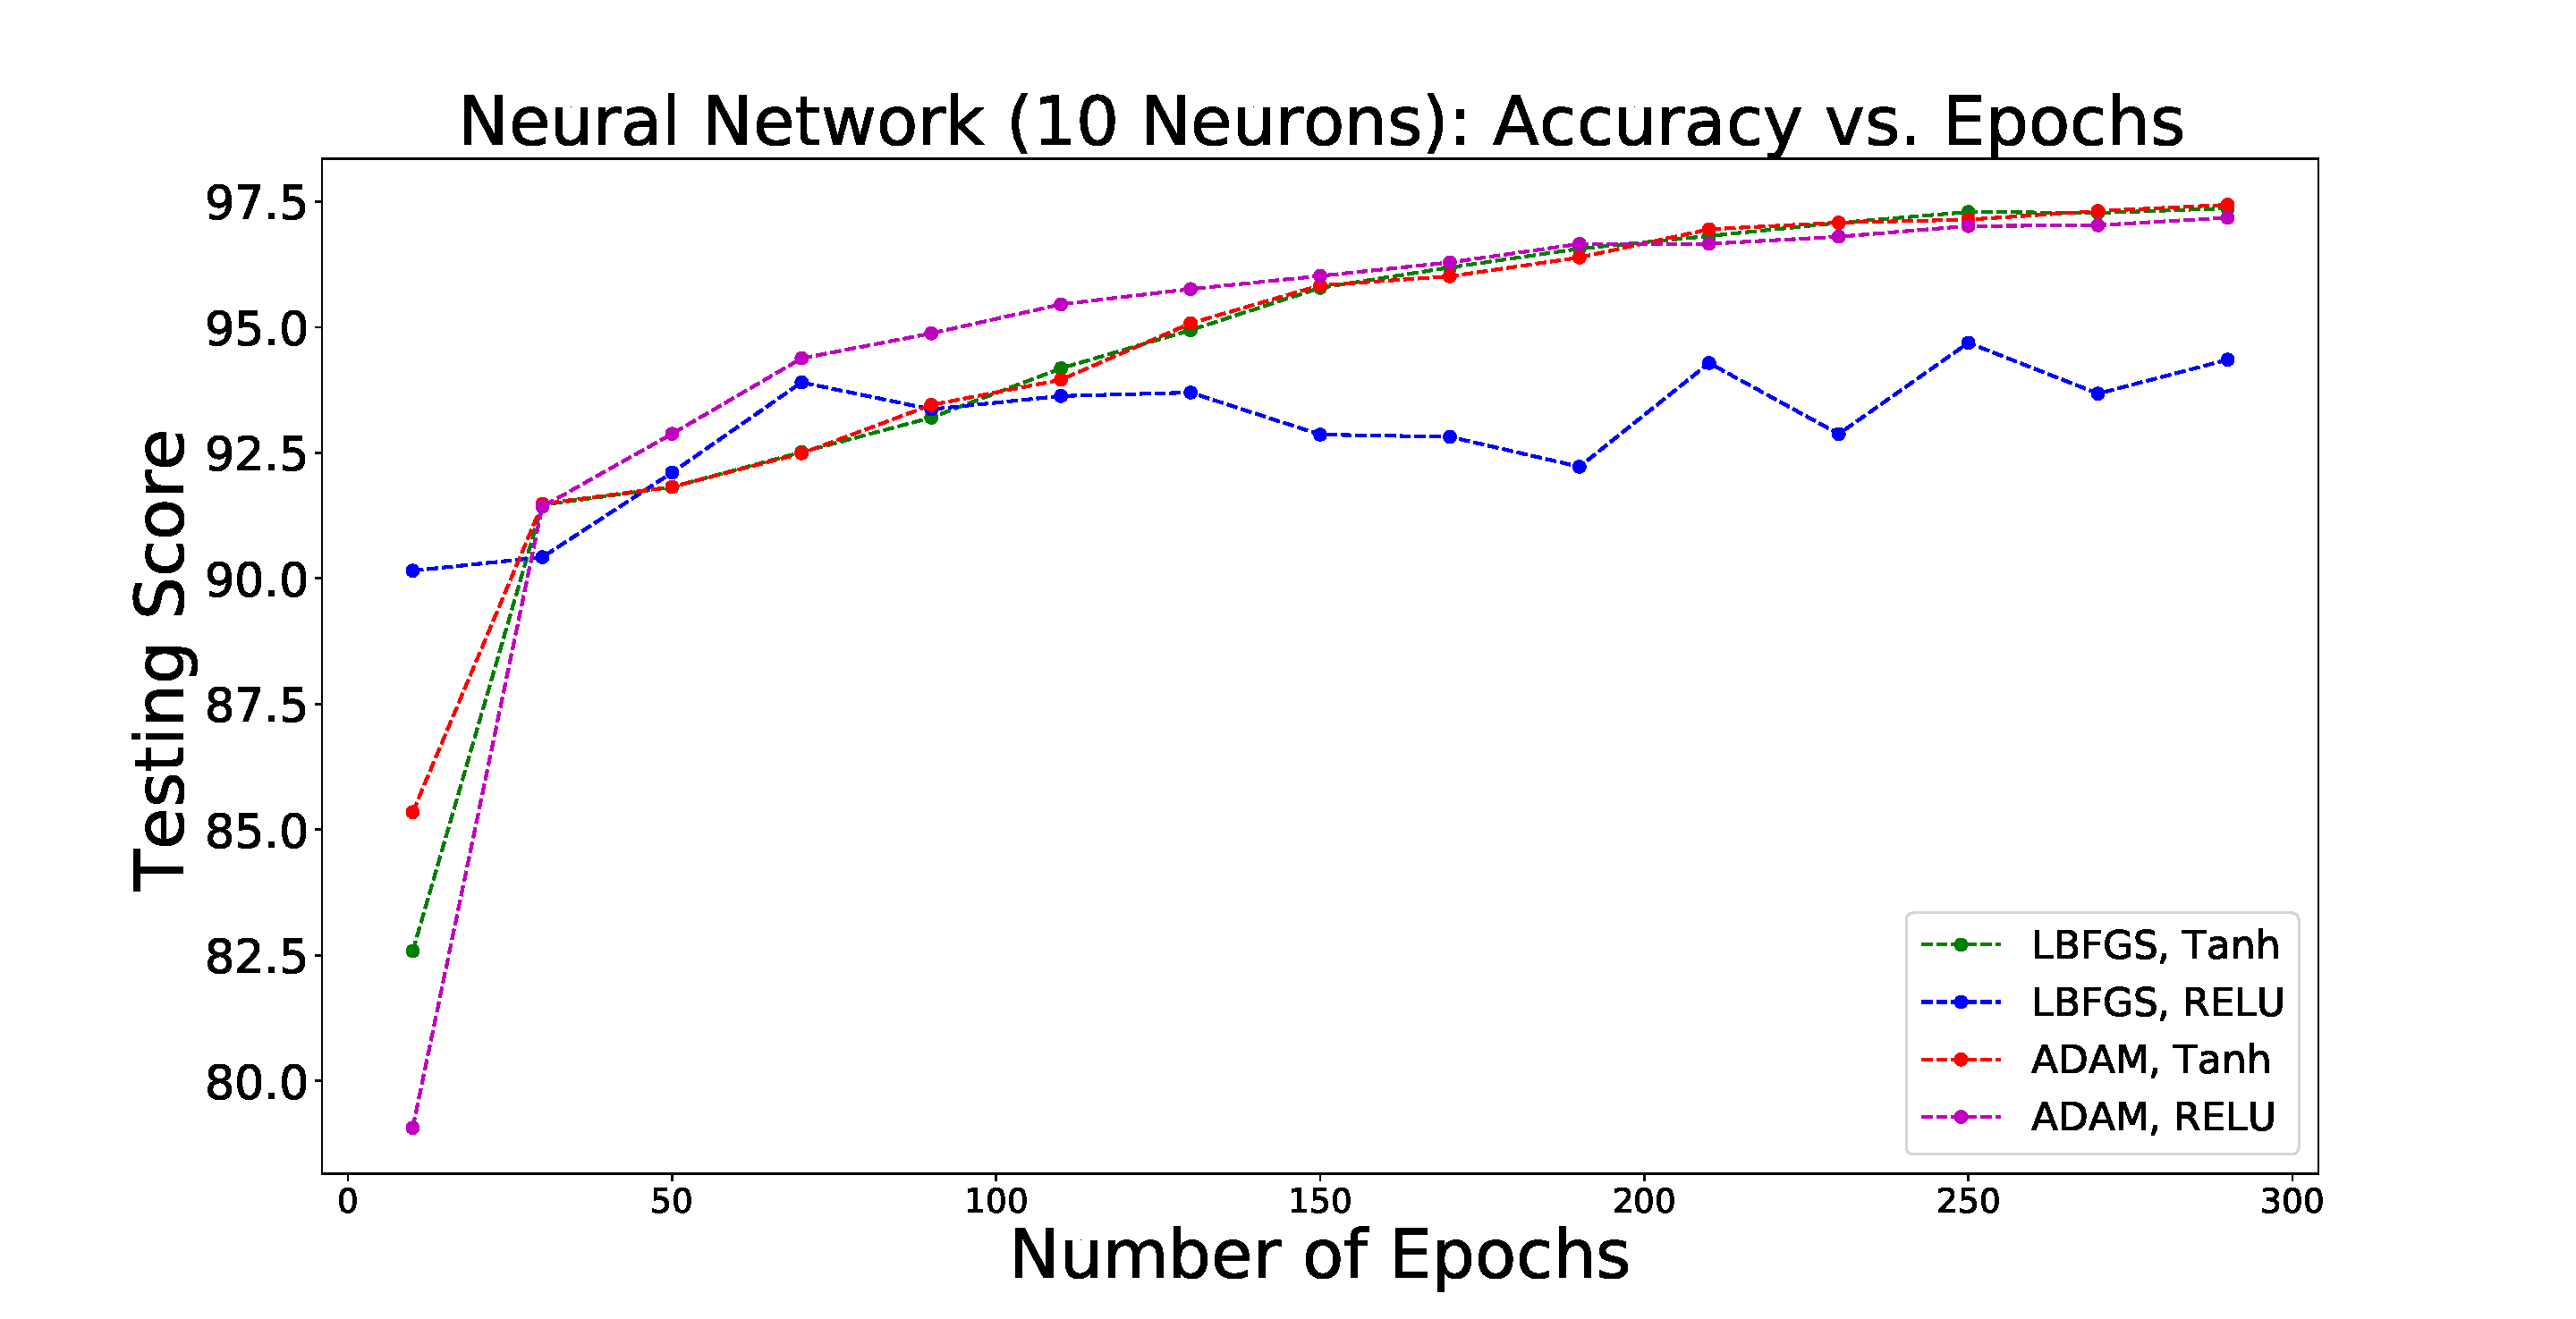
\includegraphics[width=0.5\textwidth]{plots/nn_epochs.pdf}
\caption{
Dependence on epochs for different solvers and activation functions.
}
\label{fig:NN_epochs}
\end{figure}




%\dima{Discuss L-BFGS and ADAM methods here. I don't understand where you can use tanh and relu activations, if we have only one hidden layer with classification for output.}

\begin{comment}
 we were concerned with the number of epochs that one would need to tweak, along with a dependence on the number of neurons in the hidden layers. A final improvement involved checking whether multiple hidden layers would actually add to such a classification algorithm or not.\\
As can be seen in the figure, with the specific stochastic gradient method ADAM, the number of epochs required are higher since ADAM converges slow. However, after around 200 epochs the accuracy saturates and reached the same as the lbfgs solver, which converges faster for smaller data-sets. \\
\end{comment}



%The next step was to see the effect of multiple hidden layers and number of neurons on the accuracy. In this case we found no clear dependence, and it seems as though the network doesn't overtraiin even for a higher number of neurons. This could be explained by the less number of iterations. Higher number of hidden layers added nothing more to the accuracy and serve to only over-fit the data.\\



%Like with Random forests, we also look at the probabilities here. 
We illustrate domains for NN with two input features in Figure \ref{fig:NN_domains}. 
In this case we also use only two neurons in the first hidden layer.
The figure on the top panel shows the domains after 50 epochs, which has a much less determined boundary than the
domains in the bottom panel derived for 300 epochs. 
One can also see that the separation boundary is smoother compared to the RF domains in Figure \ref{fig:RF_domains} or BDT domains in Figure \ref{fig:BDT_domains}.
%Secondly, one can clearly see how different the network behaves to the random forests before. The non-linear nature of neural networks allows it to smoothen the domain junctions (regions where there is a shift in class probabilities); this is a feature which becomes important especially when the number of training features is higher.
%\dima{As above, I don't think it makes sense to use more than 2 nodes in the hidden layer here, since there are only two input features.} 

For our final model we chose 2 hidden layer with 10 neurons in the first hidden layer and 1 neuron in the second hidden layer. We chose 300 epochs with ADAM solver. The activation function after the first hidden layer is tanh.


\begin{figure}[h]
%\centerin
\hspace*{-1cm}
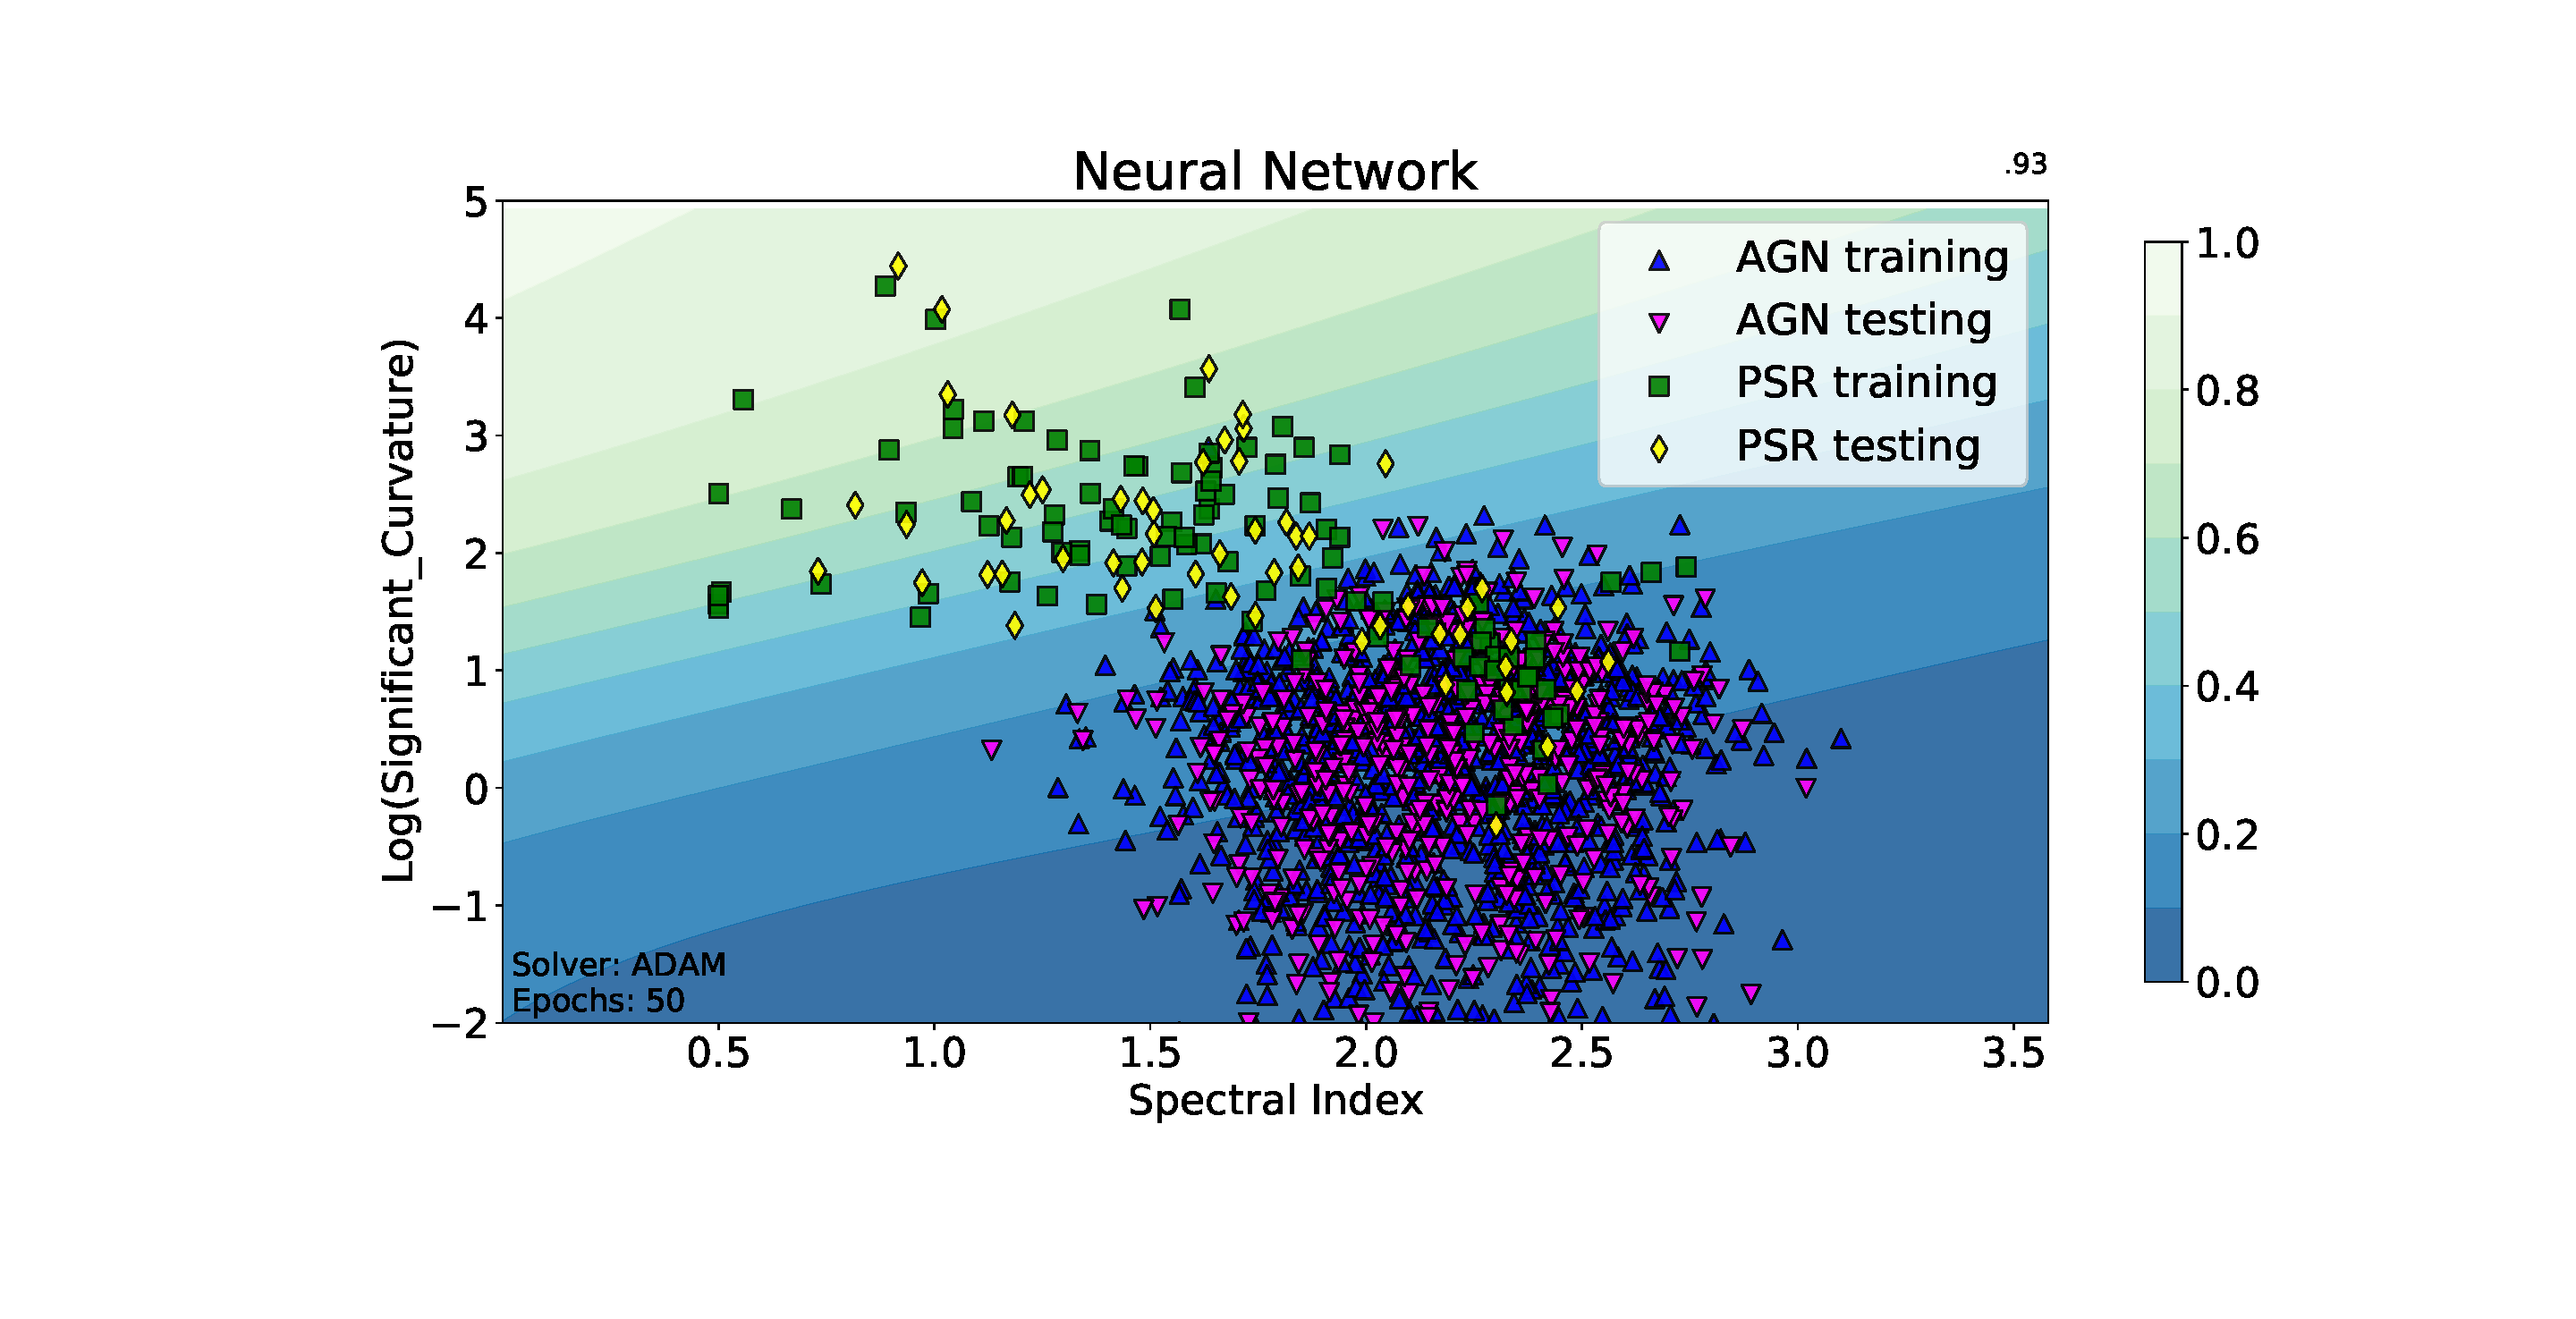
\includegraphics[width=0.55\textwidth]{plots/classification_domains/nn_adam_10_tanh_50_final.pdf}
\hspace*{-1cm}
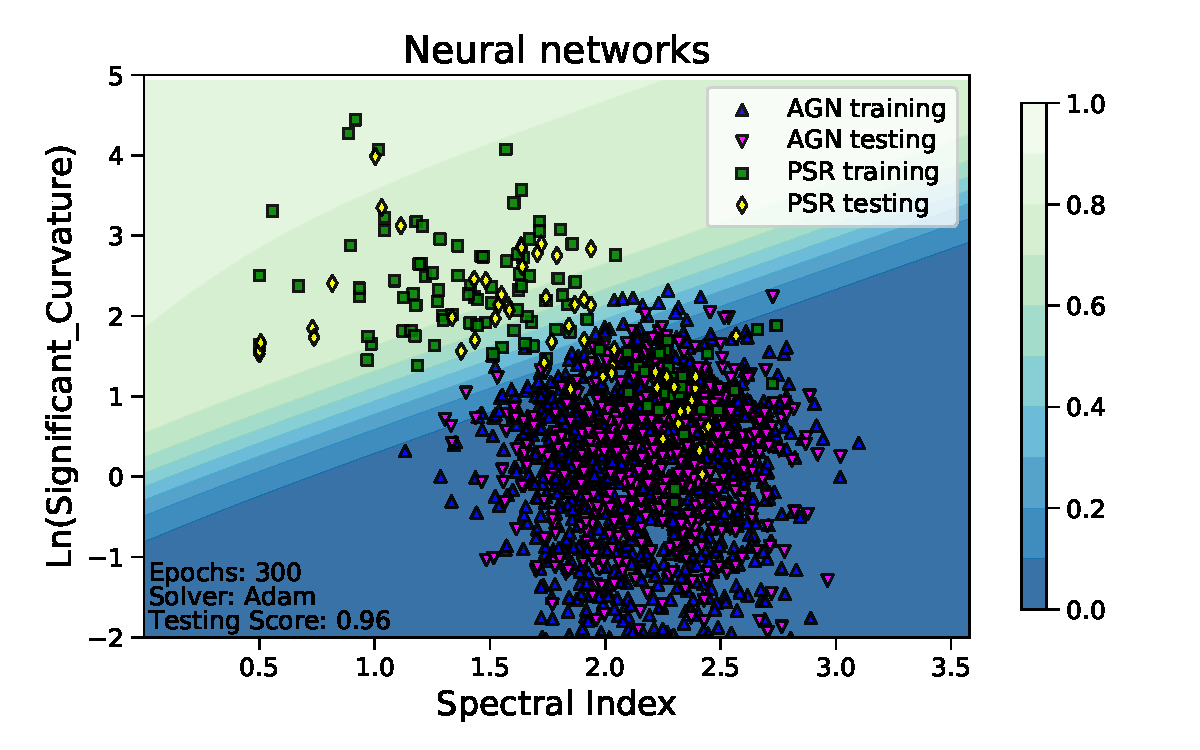
\includegraphics[width=0.55\textwidth]{plots/classification_domains/nn_adam_10_tanh_300_final.pdf}
\caption{Classification Domains for Neural Networks for the same complexity of 2 Neurons and tanh activation, using ADAM solver. }
\label{fig:NN_domains}
\end{figure}

\subsection{Logistic Regression}

As we have discussed in Section \ref{sec:class_alg}, 
the probability to belong to class 1 or 0 in LR is represented by the sigmoid function
$p_1(x) = 1 - p_0(x) = \frac{e^{m(x)}}{1 + e^{m(x)}}$ (Equation \ref{eq:logit}),
where $m(x)$ is a function of input features $x$.
The complexity of the model is given by the number of parameters in $m(x)$.
We have considered two cases for $m(x)$: linear and quadratic function of the input features $x$.
Quadratic multinomials $m(x)$ resulted in similar accuracy as a linear function $m(x)$.
Consequently, we have restricted our attention to linear functions $m(x) = \sum_{k = 1}^{10} f_k x_k$.
In Figure \ref{fig:LR_accuracy} we show the accuracy of the LR method as a function of the number of iteractions
for different solvers, e.g., LBFGS (discussed in the NN section), SAG (Stochastic Average Gradient), SAGA (a variant of SAG),
and liblinear (a special solver for LR and support vector machine classifications).
As one can see from Figure \ref{fig:LR_accuracy}, all solvers have similar performance with the LBFGs slightly outperforming the other solvers.
The top panel shows results for unweighted input data, while for the lower panel we have weights inversely proportional to the number
of elements in the class, which we have used in the discussion of the RF algorithm in Section \ref{sec:rf}.
It is interesting to note that weighted input data (lower panel in Figure \ref{fig:LR_accuracy}) give about 3\% decrease in accuracy relative to unweighted data (upper panel in Figure \ref{fig:LR_accuracy}).
For the final classification we will use LBFGs solver with 200 iterations.

In order to illustrate the probability domains in LR, we show the classification with two features (LBFGs, 200 iterations)
in Figure \ref{fig:LR_domains}. The domains look similar to the domains in the NN case (Figure \ref{fig:NN_domains}).

\begin{figure}[h]
%\centerin
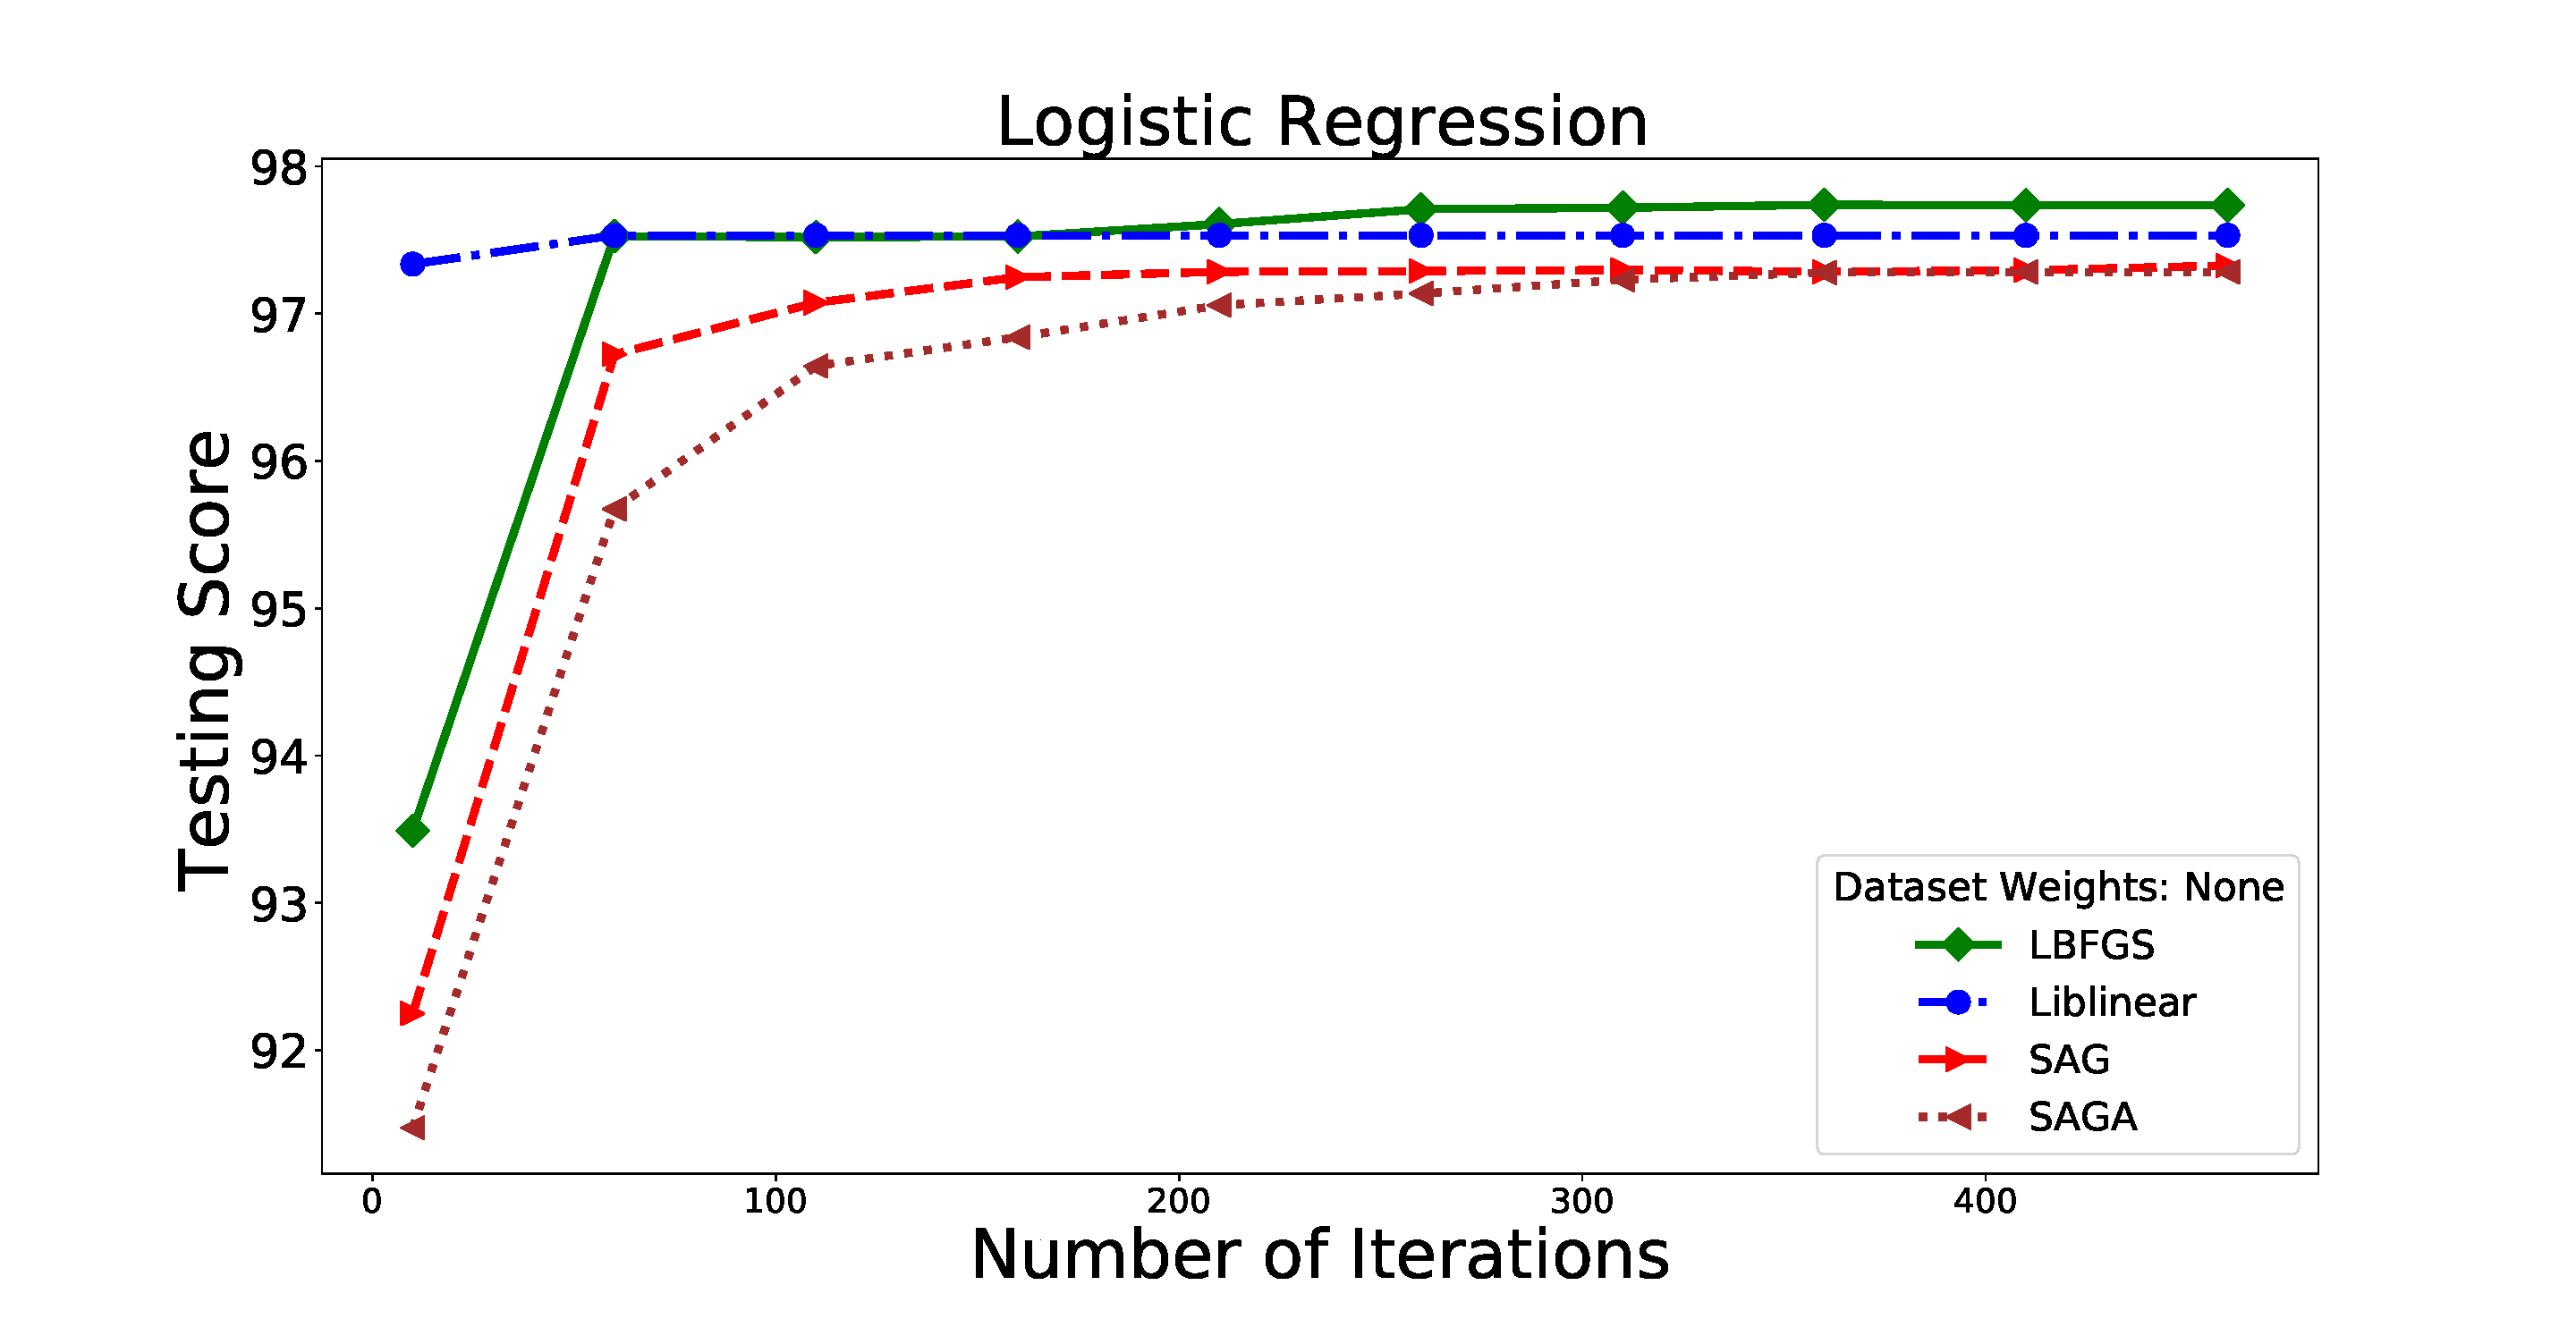
\includegraphics[width=\twopicsp\textwidth]{plots/lr_train.pdf}
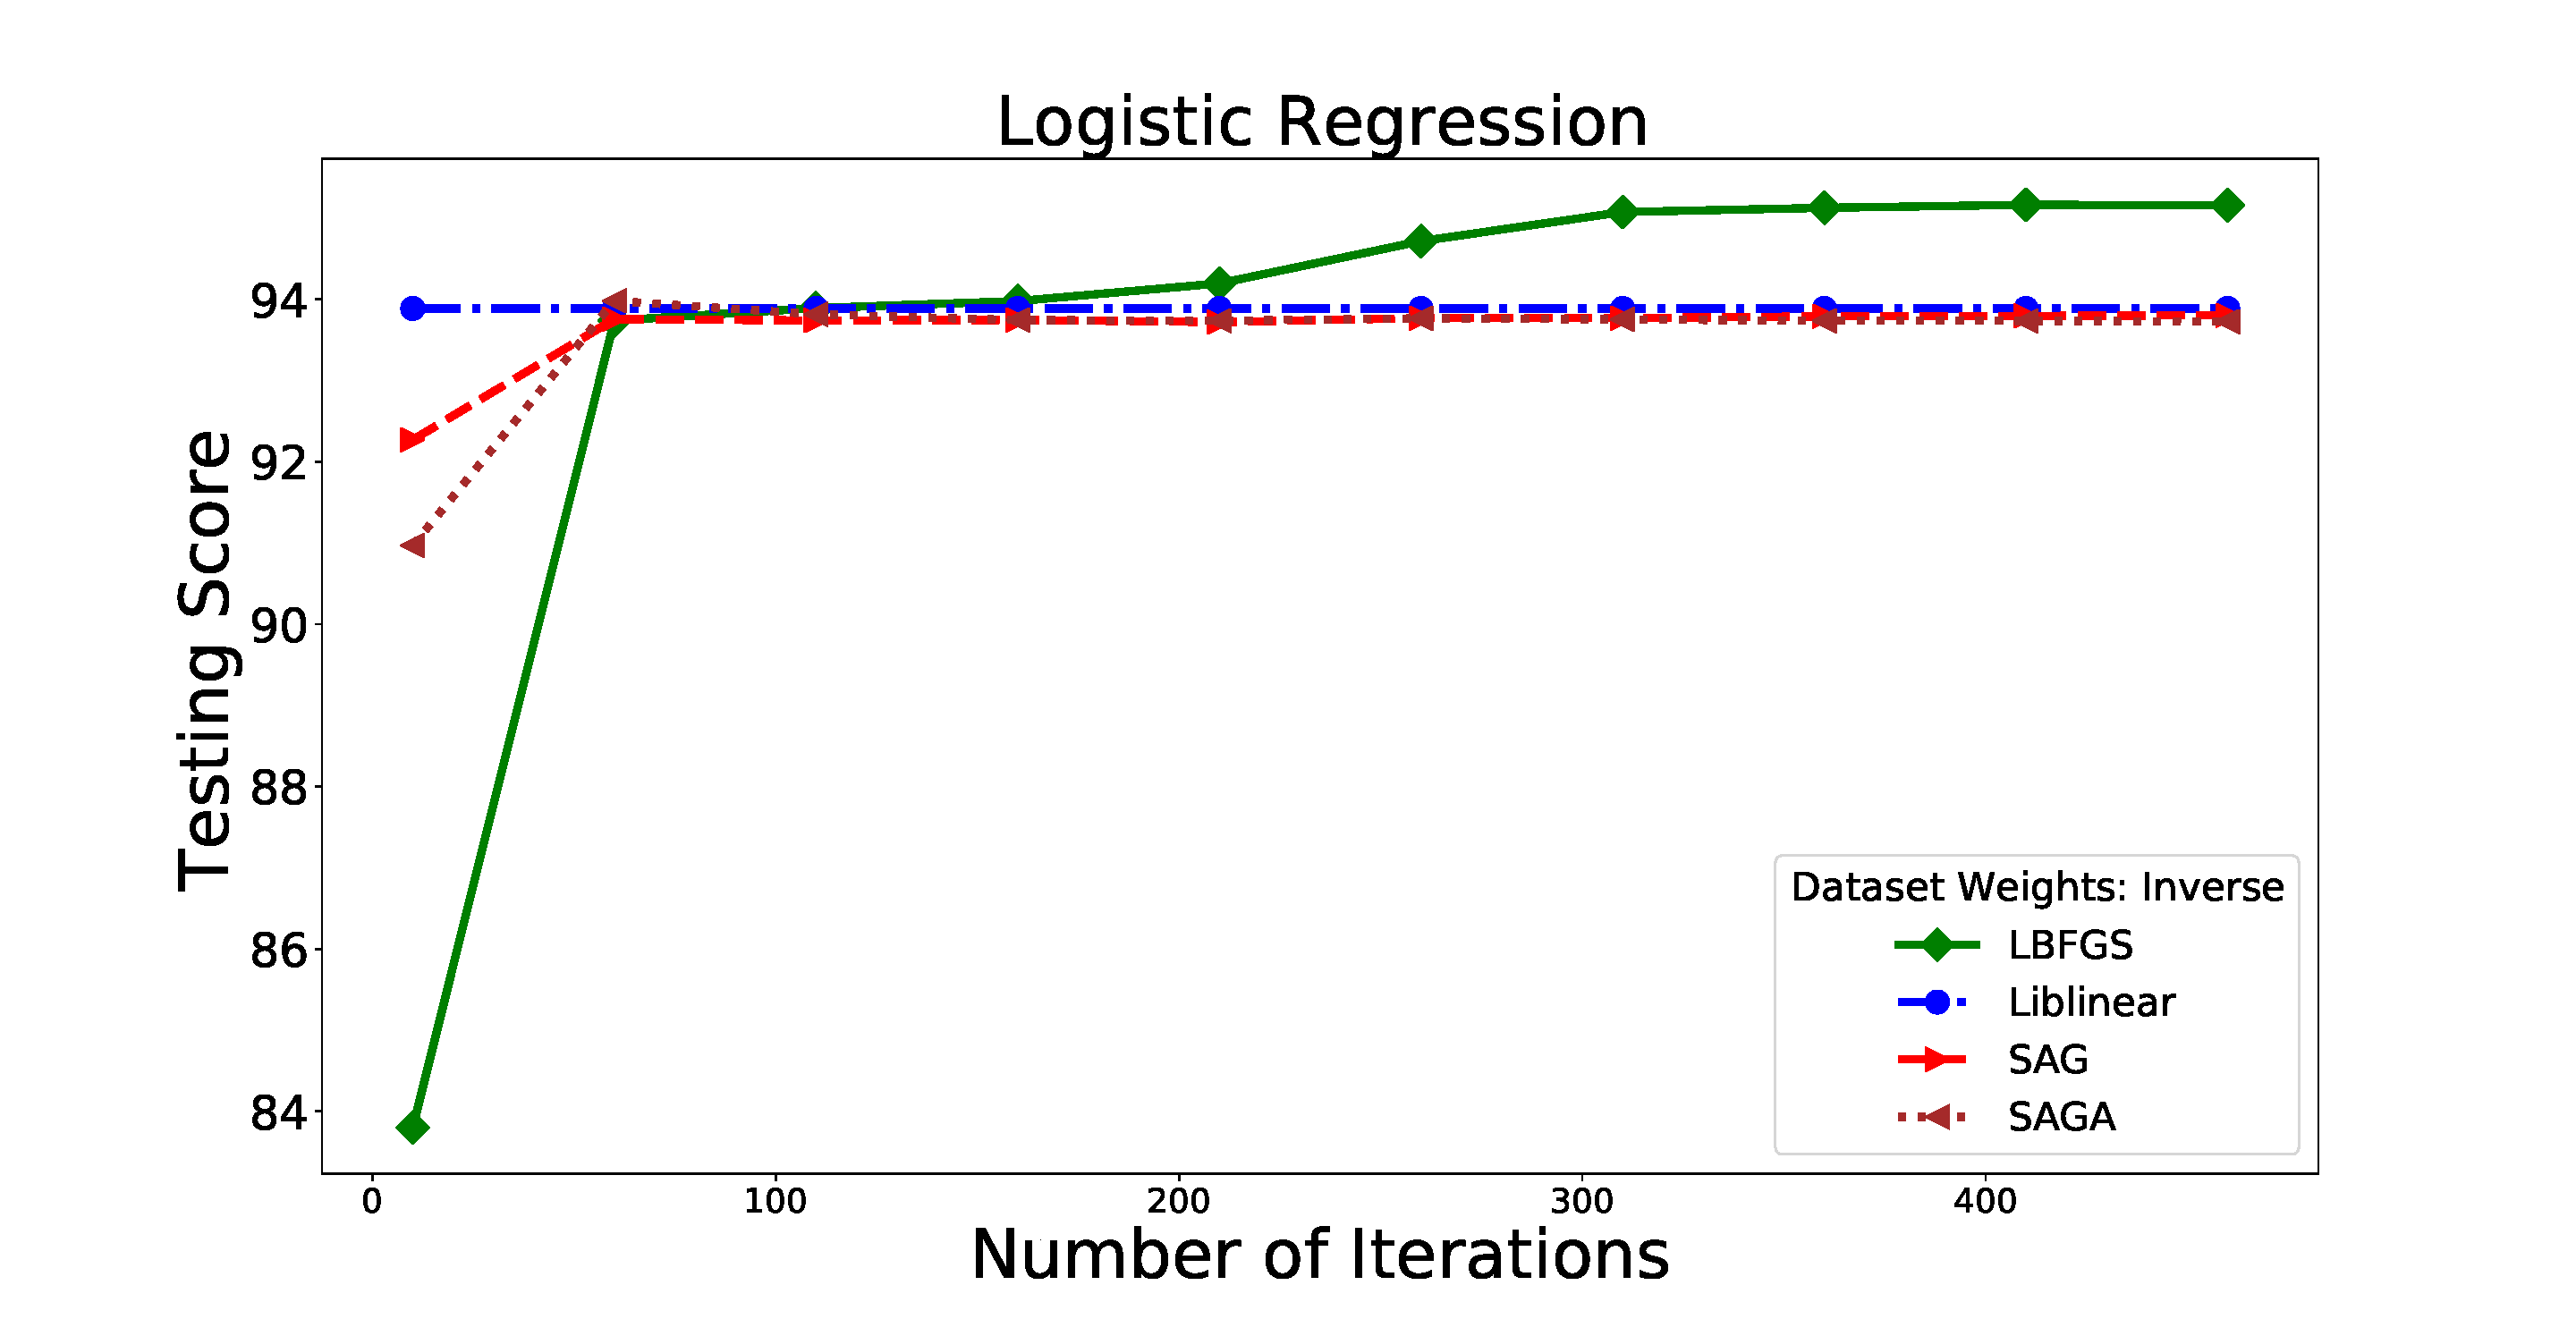
\includegraphics[width=\twopicsp\textwidth]{plots/lr_train_weights.pdf}
\caption{Dependence of LR accuracy on the number of iterations for different solvers. The accuracy for unweighted input data (upper panel) is about 3\% better than the accuracy in the case of inverse weighting (lower panel).}
\label{fig:LR_accuracy}
\end{figure}



\begin{figure}[h]
%\centerin
\hspace*{-1cm}
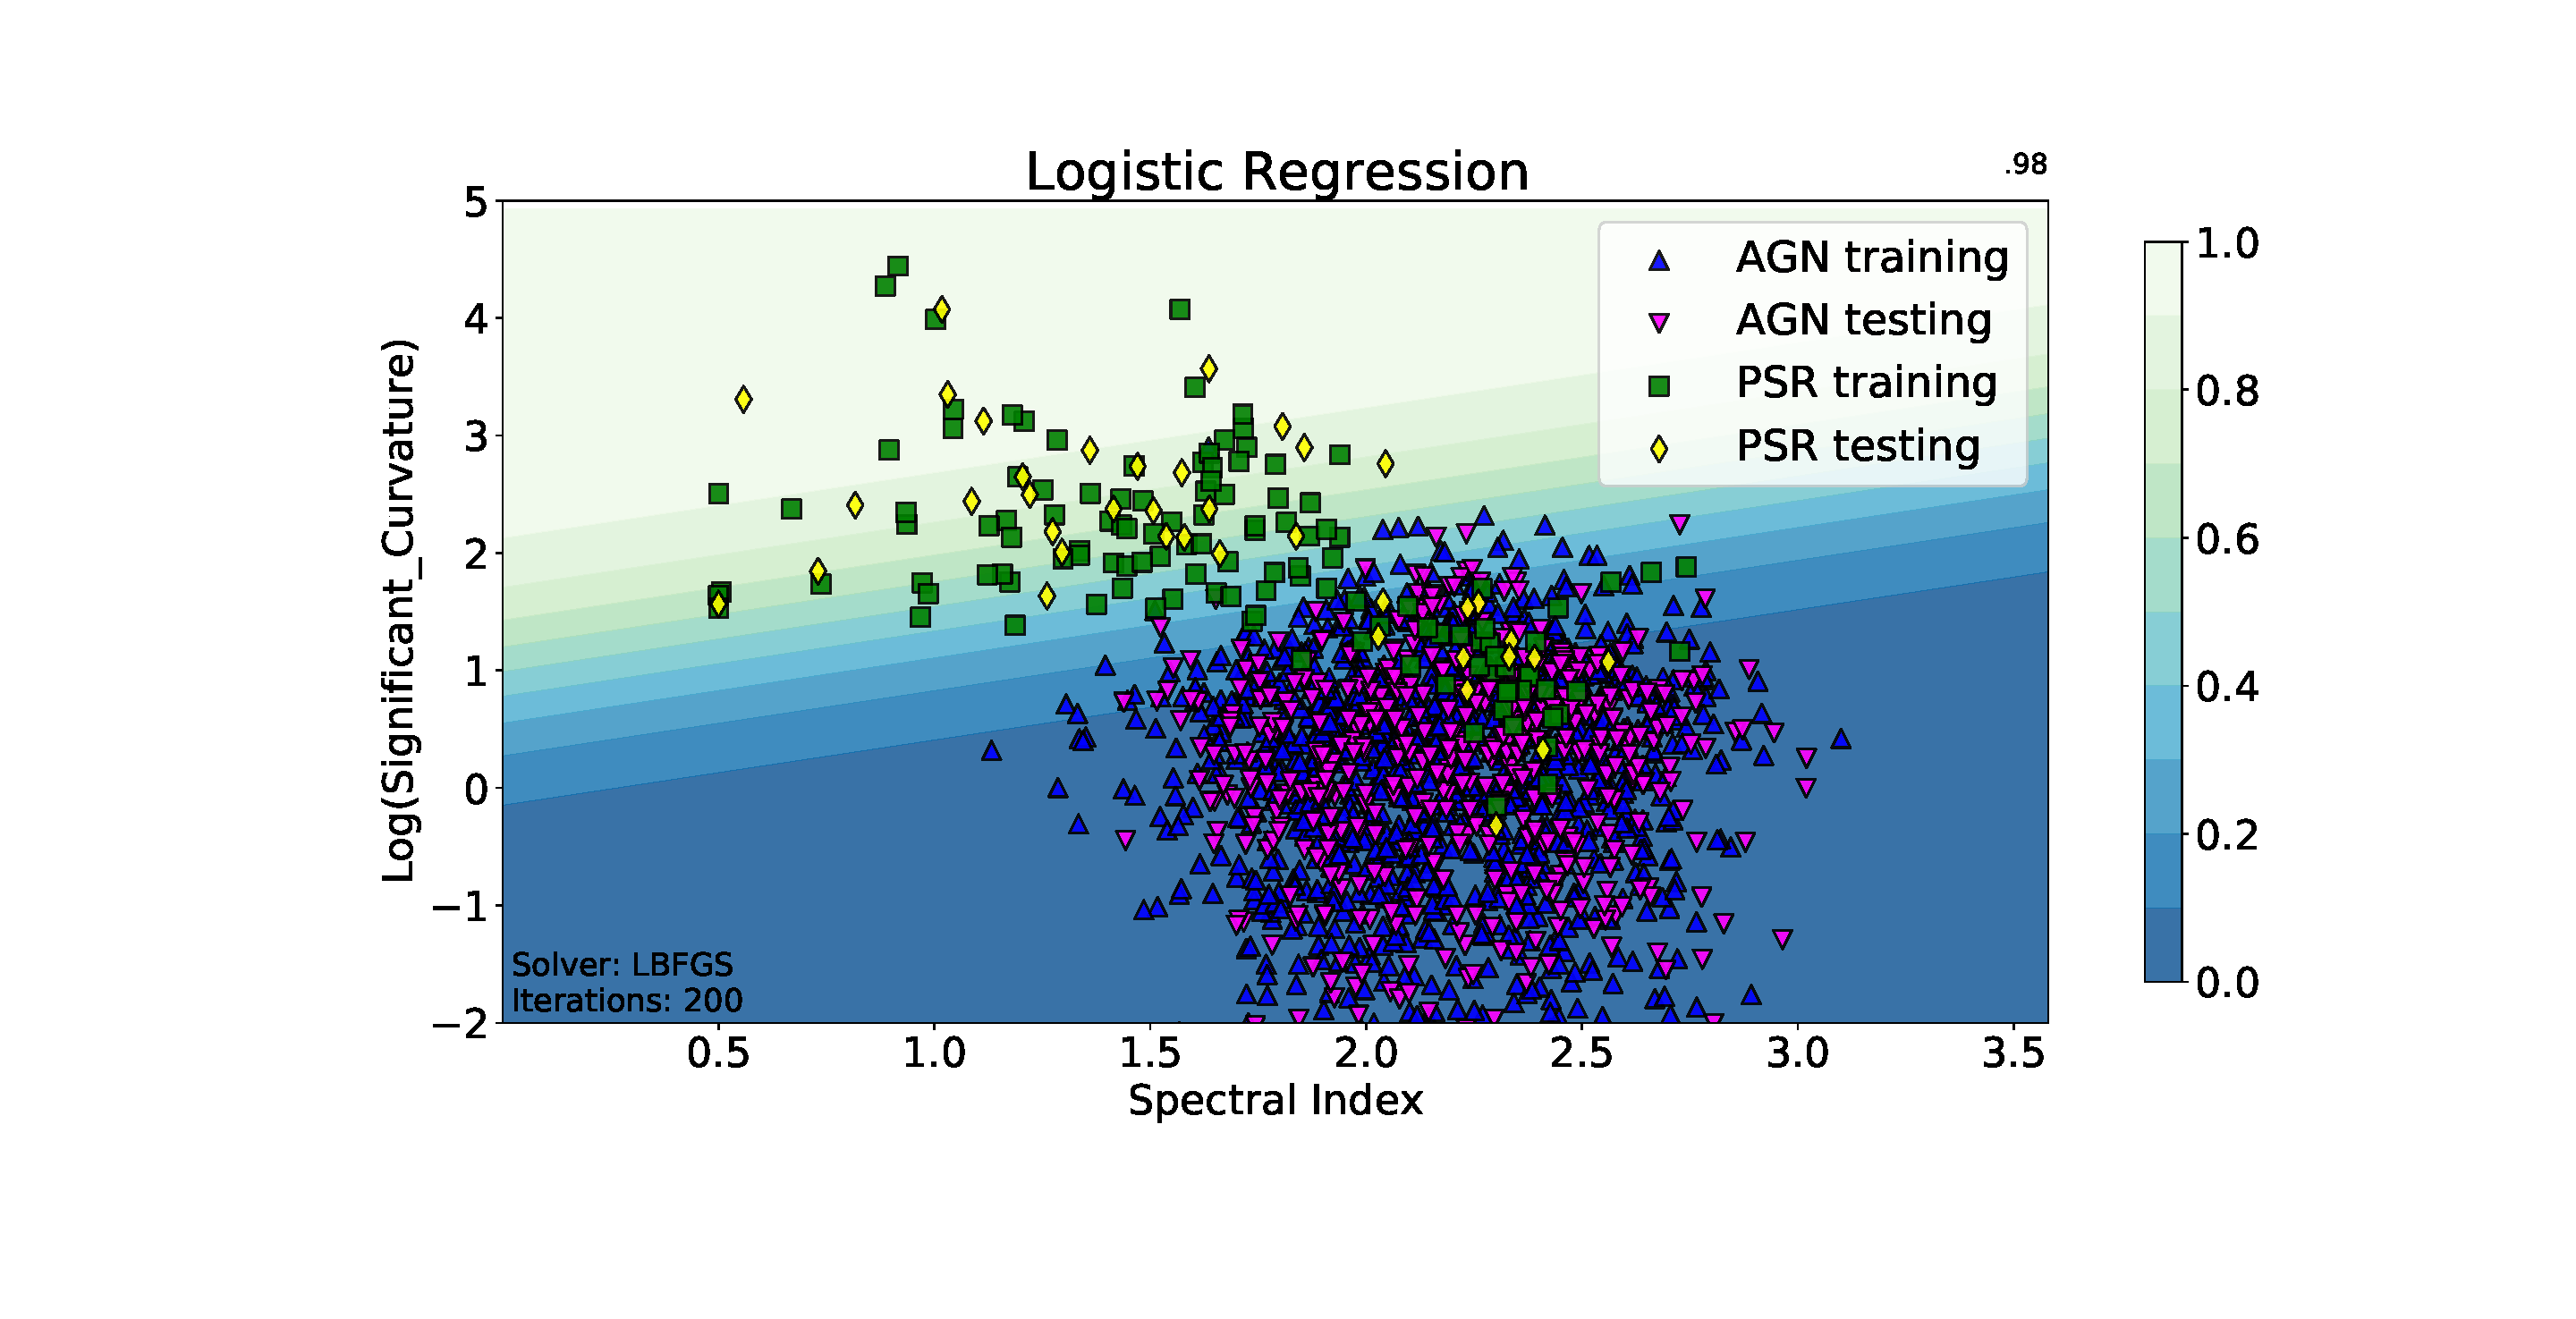
\includegraphics[width=0.6\textwidth]{plots/classification_domains/lr_200_lbfgs.pdf}
%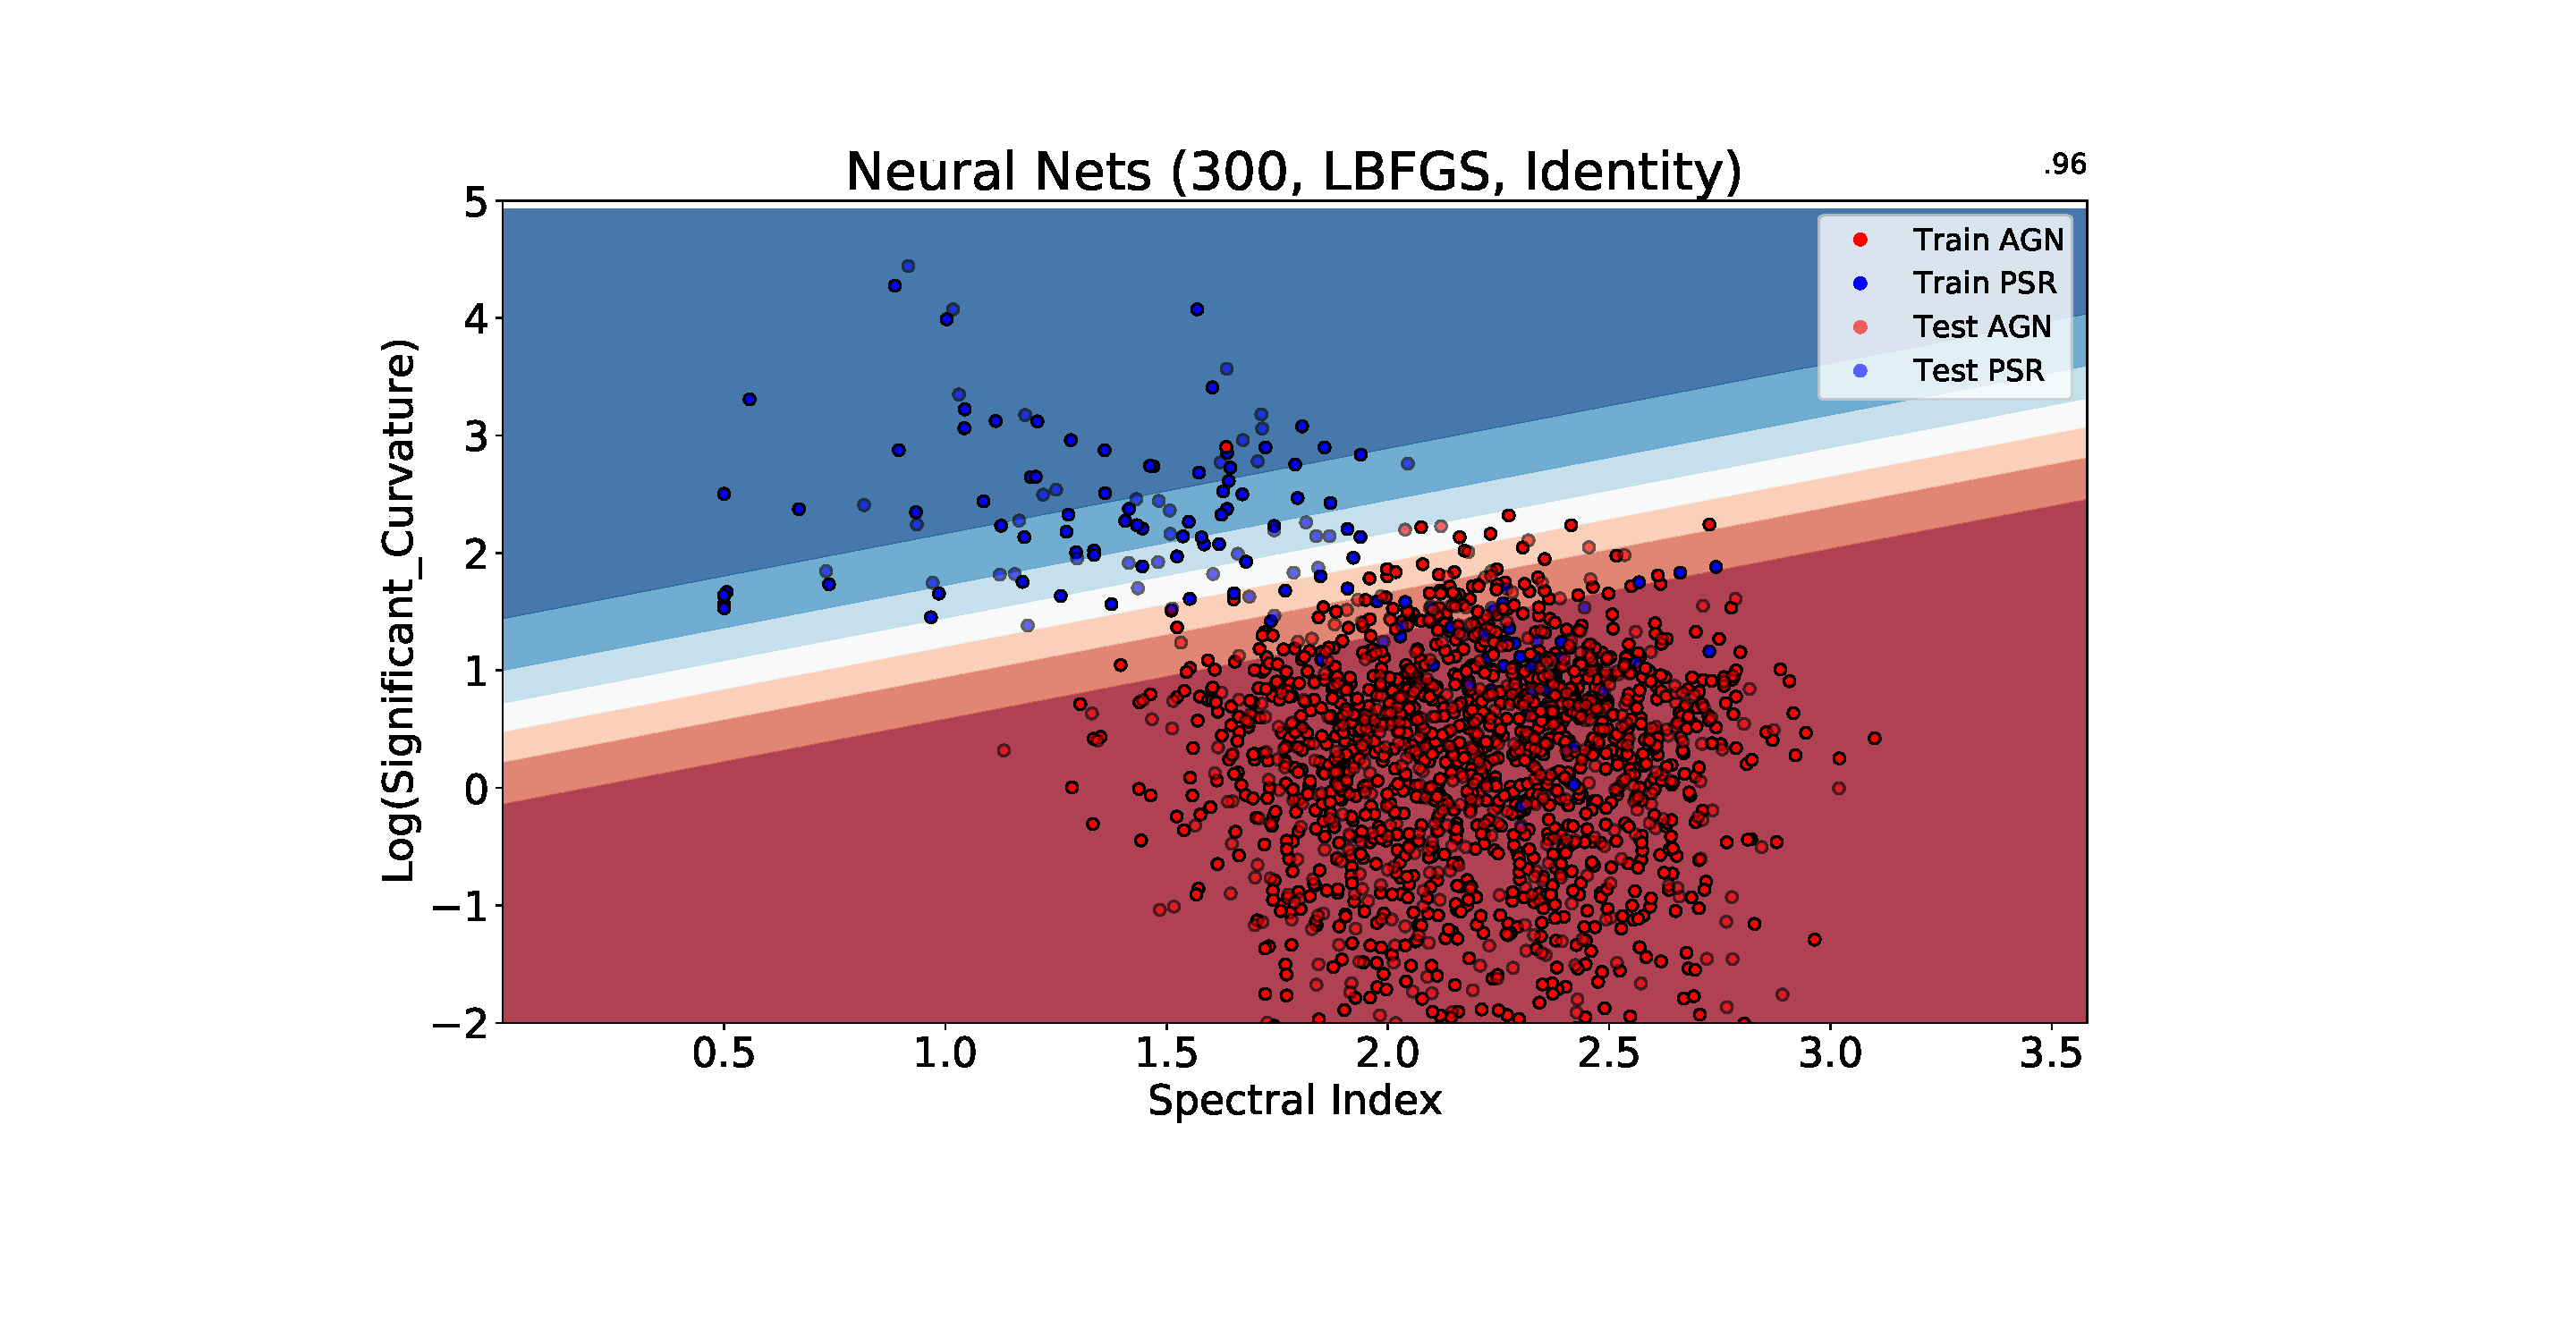
\includegraphics[width=\twopicsp\textwidth]{plots/classification_domains/NN_300_LBFGS_Identity.pdf}
\caption{Classification domains for LR with two features.}
\label{fig:LR_domains}
\end{figure}


